%%%%%%%%%%%%%%%%%%%%%%%%%%%%%%%%%%%%%%%%%%%
%%% DOCUMENT PREAMBLE %%%
\documentclass[12pt, a4paper, twoside]{report}
\usepackage[english]{babel}
\usepackage[square,numbers]{natbib}
\usepackage{url}
\usepackage[utf8x]{inputenc}
\usepackage{amsmath}
\usepackage{graphicx}
\usepackage{wrapfig}
\usepackage{parskip}
\usepackage{fancyhdr}
\usepackage{vmargin}
\usepackage[table]{xcolor}
\usepackage{setspace}
\usepackage{array}
\usepackage{setspace}
\usepackage[colorlinks]{hyperref}
\usepackage{calc}
\usepackage{mwe}
\usepackage{caption}
\usepackage{subcaption}
\usepackage{enumitem}
\usepackage{booktabs}
\usepackage{listings}
\usepackage{wallpaper}
\usepackage{longtable}


\usepackage{caption}
\captionsetup[longtable]{skip=-1.53\baselineskip}
\captionsetup[figure]{aboveskip=0.2\baselineskip, belowskip=-1.3\baselineskip}
\captionsetup[wrapfigure]{aboveskip=0.2\baselineskip, belowskip=-1.3\baselineskip}

\bibliographystyle{abbrvnat}

% use it to wrap URI templates 
%\newcommand*{\ptr}[1]{\footnotesize\ttfamily #1}

\newcommand{\cincludegraphics}[2][]{%
	\sbox0{\includegraphics[#1]{#2}}%
	\ht0=\dimexpr\ht0+3pt\relax
	\dp0=3pt
	\splitcell{\box0}%
}
\newcommand{\splitcell}[1]{%
	\begin{tabular}{@{}c@{}}#1\end{tabular}%
}

\let\svparbox\parbox
\renewcommand\parbox[3][c]{\svparbox[#1]{#2}{\strut#3\strut}}

\DeclareTextFontCommand{\ptr}{\footnotesize\ttfamily}
\DeclareTextFontCommand{\texttt}{\footnotesize\ttfamily}

\usepackage[
type={CC},
modifier={by},
version={4.0},
]{doclicense}

\hypersetup{
	colorlinks,
	citecolor=black,
	filecolor=black,
	linkcolor=black,
	urlcolor=black,
	colorlinks=true, %set true if you want colored links
	linktoc=all,     %set to all if you want both sections and subsections linked
%	linkcolor=blue,  %choose some color if you want links to stand out
}
\setmarginsrb{3 cm}{2.5 cm}{3 cm}{2.5 cm}{1 cm}{1.5 cm}{1 cm}{1.5 cm}

%\graphicspath{{figures/}}

%\title{1}								
%% Title
%\author{Eugeniu Costetchi}						
%% Author
%\date{today's date}
%% Date

%\makeatletter
%\let\thetitle\@title
%\let\theauthor\@author
%\let\thedate\@date
%\makeatother

%\pagestyle{fancy}
%\fancyhf{}
%\lhead{\DelAuthor}
%\rhead{\DelTitle}
%\cfoot{\thepage}

%%%%%%%%%%%%%%%%%%%%%%%%%%%%%%%%%%%%%%%%%%%%
\begin{document}

%%%%%%%%%%%%%%%%%%%%%%%%%%%%%%%%%%%%%%%%%%%%%%%%%%%%%%%%%%%%%%%%%%%%%%%%%%%%%%%%%%%%%%%%%
%Title Page
%%%%%%%%%%%%%%%%%%%%%%%%%%%%%%%%%%%%%%%%%%%%%%%%%%%%%%%%%%%%%%%%%%%%%%%%%%%%%%%%%%%%%%%%%
%!TEX root = deliverable49.tex

%%%%%%%%%%%%%%%%%%%%%%%%%%%%%%%%%%%%%%%%%%%%%%%%%%%%%%%%%%%%%%%%%%%%%%%%%%%%%%%%%%
% First Page
%%%%%%%%%%%%%%%%%%%%%%%%%%%%%%%%%%%%%%%%%%%%%%%%%%%%%%%%%%%%%%%%%%%%%%%%%%%%%%%%%%

% placing a text box at specific position in the page
% usage: \placetextbox{<horizontal pos>}{<vertical pos>}{<stuff>}
% source: https://tex.stackexchange.com/questions/24663/how-to-place-a-floating-text-box-at-a-specified-location-in-page-coordinates
\newcommand{\placetextbox}[3]{% \placetextbox{<horizontal pos>}{<vertical pos>}{<stuff>}
	\setbox0=\hbox{#3}% Put <stuff> in a box
	\AddToShipoutPictureFG*{% Add <stuff> to current page foreground
		\put(\LenToUnit{#1\paperwidth},\LenToUnit{#2\paperheight}){\vtop{{\null}\makebox[0pt][c]{#3}}}%
	}%
}%

% defining the page metadata variables
\newcommand{\DelAcronym}{ePO}
\newcommand{\DelTitle}{Asset Publication Lifecycle Architecture}
\newcommand{\DelNumber}{WP 1.1}
\newcommand{\DelVersion}{1.0}
\newcommand{\DelCorporateAuthor}{Publications Office of the European Union}
\newcommand{\DelAuthor}{Eugeniu Costetchi}
\newcommand{\DelReviewer}{Denis Dechandon and Willem Van Gemert}
\newcommand{\DelDate}{25 September 2020}
%\newcommand{\DelFilename}{wp1-1-ontology-architecture}
\newcommand{\DelInitiative}{Initiative for digital transformation in the Metadata and Reference Data Sector of the Publications Office of the European Union}
\newcommand{\DelPreparation}{This report was prepared for the Publications Office of the European Union by \mbox{Infeurope}.}
\newcommand{\DelReaders}{sector management, business and technical staff, stakeholders, enterprise architects, software developers, project partners}
\newcommand{\DelCopyright}{\textsuperscript{\textcopyright} European Union, 2020 }


\pagestyle{empty}


\begin{titlepage}
\begin{center}

\begin{center}
	\begin{center}
		\setlength{\tabcolsep}{0pt}
%		\begin{tabular}{>{\raggedleft}m{3.5cm}>{\centering}m{\dimexpr\textwidth - 8cm\relax}>{\raggedright}m{3.5cm}}
%			
\includegraphics[width=1.15\linewidth]{images/logos/OP-50years-EN}%			
%			&%
%%			\textbf{\large dfs} \\[5pt]%
%%			\textbf{\large sdfs}%
%			&%
%			
\includegraphics[width=\linewidth]{images/logos/infeurope-blue-logo}%
%		\end{tabular}
	
\includegraphics[width=0.45\linewidth]{docs/architecture/images/logos/EU-OP.png}
\end{center}

\ThisLRCornerWallPaper{1}{images/background}

%  
\includegraphics[scale=.71]{images/logos/OP-50years-EN}
  \vspace{2mm}

  \end{center}
  \vspace{5cm}
  \textbf{{\large \DelInitiative\\}}
  \vspace{2cm}
  
  \begin{spacing}{2.5}
    \textbf{\Huge \DelTitle}\\ \vspace{2cm}
%    {\large Deliverable \DelNumber} \\ %\vspace{10mm} 
%	 {\large \DelAuthor} \\ %\vspace{10mm} 
%	 {\large \DelDate} \\ %\vspace{10mm} 
%    {\large Version \DelVersion}
  \end{spacing}
  
  
  
  \vspace*{\fill}  
   
%  {\footnotesize \doclicenseText\\\doclicenseIcon }
%  \doclicenseText  
  
  \newcolumntype{C}{ >{\arraybackslash} m{3cm} }

\end{center}
\end{titlepage}

\clearpage


%%%%%%%%%%%%%%%%%%%%%%%%%%%%%%%%%%%%%%%%%%%%%%%%%%%%%%%%%%%%%%%%%%%%%%%%%%%%%%%%%%
% Second Page 
%%%%%%%%%%%%%%%%%%%%%%%%%%%%%%%%%%%%%%%%%%%%%%%%%%%%%%%%%%%%%%%%%%%%%%%%%%%%%%%%%%
\setlength{\headheight}{1cm}
\setlength{\footskip}{18mm}
\addtolength{\textheight}{-\footskip}
\pagestyle{empty}

\clearpage

\section*{Disclaimer}
The views expressed in this report are purely those of the Author(s) and may not, in any circumstances, be interpreted as stating an official position of the European Union. The European Union does not guarantee the accuracy of the information included in this study, nor does it accept any responsibility for any use thereof. Reference herein to any specific products, specifications, process, or service by trade name, trademark, manufacturer, or otherwise, does not necessarily constitute or imply its endorsement, recommendation, or favouring by the European Union. 


\vspace*{\fill}  
%\vspace{4cm}

\textbf{\footnotesize \DelPreparation}

\begin{flushleft}
\begin{table*}[!b]
	 \caption*{\large\textbf{Document metadata}}
	 \footnotesize
	  \begin{tabular}{p{3.6cm}p{\textwidth-5cm}}
%		\textbf{Project acronym}       &   \DelAcronym \\
%		\textbf{Project title}    &   \DelInitiative  \\ 
		\textbf{Reference} 	&   \DelNumber: \DelTitle \\	
		\textbf{Corporate Author}      &   \DelCorporateAuthor \\
		\textbf{Author}             &   \DelAuthor \\
		\textbf{Reviewers}          &   \DelReviewer \\
		\textbf{Contractor}    &   Infeurope S.A. \\
		\textbf{Framework contract}    &   10688/35368 \\	
		\textbf{Work package}  &   \DelNumber\\    				
		\textbf{Delivery date}  &   \DelDate \\    
%		\textbf{Delivery nature}     	&   Report (R) \\
%		\textbf{Dissemination licence} 	&   \doclicenseLongNameRef \\
%		\textbf{Filename}           	&   \DelFilename\\
		\textbf{Suggested readers}    	&   \DelReaders \\
	\end{tabular}
\end{table*}
\end{flushleft}

%\vspace*{\fill}  

\placetextbox{0.37}{0.027}{\footnotesize \DelCopyright}

\clearpage
\section*{Abstract}

    In the European Union, the public sector is one of the most data-intensive sectors. The re-use of open data can contribute, for example, to the growth of the European economy, the development of artificial intelligence and overcoming societal challenges.

	Given the increasing importance of data standards for the EU institutions, a number of initiatives driven by the public sector, industry and academia have been kick-started in recent years. Some have grown organically, while others are the result of standardisation work. The vocabularies and semantics that they are introducing, together with the technologies that they are using, all differ. These differences hamper data interoperability and thus its reuse by them or by the wider public. This creates the need for a common data standard for publishing public reference data and models, hence allowing data from different sources to be easily accessed, linked, and consequently reused.
	
	The PSI directive across the EU calls for open, unobstructed access to public data in order to improve transparency and to boost innovation via the reuse of public data. The reference data maintained and published by the PO has been identified as data with a high-reuse potential. Therefore, making this data available in machine-readable formats, as well as following the data as a service paradigm, are required in order to maximise its reuse.
	
	In this context, the Publications Office of the European Union maintains and publishes an ever-increasing number of reference data assets which are vital in the context of inter-institutional information exchange. With regards to reference data, the PO provides an ever-increasing number of services to the main institutional stakeholders and with the aim to extend them to a broader public, enabling active or passive participation in the reference data life cycle, standardisation and harmonisation.
	
	This document provides a working definition of the architectural stance and design decisions that are to be adopted for the asset publication life-cycle process. This process is materialised as the publication workflow and is currently employed by the Standardisation Unit (SU) at the Publications Office of the European Union (PO).
	
% 	In this document we (a) establish the baseline architecture, supported by  strategic and motivational information; and (b) develop a target architecture guiding the digital transformation processes towards new technologies. This constitutes a natural evolution in response to changing mission needs defined by SU management, and also takes into consideration the strategic directions proposed by the PO, the European Commission (EC) and the European Parliament (EP) as presented below.
\clearpage
%XXX


%%%%%%%%%%%%%%%%%%%%%%%%%%%%%%%%%%%%%%%%%%%%%%%%%%%%%%%%%%%%%%%%%%%%%%%%%%%%%%%%%%%%%%%%%
\pagestyle{fancy}
\fancyhf{}
%%\rhead{\slshape\DelAuthor}
%%\rhead{\slshape{\DelInitiative}}
%\rhead{\slshape\nouppercase{\rightmark}}
%\lhead{\slshape\nouppercase{\leftmark}}
\fancyhead[RE]{\slshape\nouppercase{\rightmark}}      % Chapter in the right on even pages
\fancyhead[LO]{\slshape\nouppercase{\leftmark}}     % Section in the left on odd pages
\cfoot{\thepage}

%%%%%%%%%%%%%%%%%%%%%%%%%%%%%%%%%%%%%%%%%%%%%%%%%%%%%%%%%%%%%%%%%%%%%%%%%%%%%%%%%%%%%%%%%


%%% Local Variables: 
%%% mode: latex
%%% TeX-master: "main"
%%% End: 


%%%%%%%%%%%%%%%%%%%%%%%%%%%%%%%%%%%%%%%%%%%%%%%%%%%%%%%%%%%%%%%%%%%%%%%%%%%%%%%%%%%%%%%%%

\tableofcontents
\vspace*{\fill}  
\pagebreak


%\renewcommand{\thesection}{\arabic{section}} % this provides numbering with sections only, without the chapers
%%%%%%%%%%%%%%%%%%%%%%%%%%%%%%%%%%%%%%%%%%%%%%%%%%%%%%%%%%%%%%%%%%%%%%%%%%%%%%%%%%%%%%%%%
% Content sections follow
%%%%%%%%%%%%%%%%%%%%%%%%%%%%%%%%%%%%%%%%%%%%%%%%%%%%%%%%%%%%%%%%%%%%%%%%%%%%%%%%%%%%%%%%% 

\section{Introduction}
\label{sec:introduction}
%	TODO: About Standardisation Unit (SU): where it is, what it currently does, and why. 

	
	This document provides a working definition of the architectural stance and design decisions that are to be adopted for the asset publication life-cycle process. This process is materialised as the publication workflow and is currently employed by the Standardisation Unit (SU) at the Publications Office of the European Union (PO).
	
	In this document we (a) establish the baseline architecture, supported by  strategic and motivational information; and (b) develop a target architecture guiding the digital transformation processes towards new technologies. This constitutes a natural evolution in response to changing mission needs defined by SU management, and also takes into consideration the strategic directions proposed by the PO, the European Commission (EC) and the European Parliament (EP) as presented below.
	
	\subsection{Background considerations}
	
	Given the increasing importance of data standards for the EU institutions, a number of initiatives driven by the public sector, industry and academia have been kick-started in recent years. Some have grown organically, while others are the result of standardisation work. The vocabularies and semantics that they are introducing, together with the technologies that they are using, all differ. These differences hamper data interoperability and thus its reuse by them or by the wider public. This creates the need for a common data standard for publishing public reference data and models, hence allowing data from different sources to be easily accessed, linked, and consequently reused.
	
	The PSI directive \cite{directive-2019/1024} across the EU calls for open, unobstructed access to public data in order to improve transparency and to boost innovation via the reuse of public data. The reference data maintained and published by the PO has been identified as data with a high-reuse potential \cite{d-high-value-assets}. Therefore, making this data available in machine-readable formats, as well as following the data as a service paradigm, are required in order to maximise its reuse.
	
	In this context, the Publications Office of the European Union maintains and publishes an ever-increasing number of reference data assets which are vital in the context of inter-institutional information exchange. With regards to reference data, the PO provides an ever-increasing number of services to the main institutional stakeholders and with the aim to extend them to a broader public, enabling active or passive participation in the reference data life cycle, standardisation and harmonisation.

	\subsection{EU trajectory towards public sector linked open data}
	
	European institutions started out to adopt Semantic Web and Linked Data technologies as part of their visions to become data-centred e-government bodies \citep{decission-456/2005/EC,decission-2015/2240}. 
	
	The EU institutions also aim for implementation of a single digital gateway to ``facilitate interactions between citizens and businesses, on the one hand, and competent authorities, on the other hand, by providing access to online solutions, facilitating the day-to-day activities of citizens and businesses and minimising the obstacles encountered in the internal market. The existence of a single digital gateway providing online access to accurate and up-to-date information, to procedures and to assistance and problem-solving services could help raise the users' awareness of the different existing online services and could save them time and expense'' \citep{directive-2018/1724}. This is well in line with earlier established goals for encouraging the open data and the re-use of public sector information \citep{directive-2013/37/EU,directive-2019/1024}.

	Many of the legacy systems used in the EU institutions use XML data format for exchange and document formats governed by the XSD schemes \citep{xsd1.1-spec}. The aim is to evolve technologically so that both existing and new systems are capable to operate with semantic data representations using RDF \citep{rdf11}, OWL \citep{owl2.0,owl2}, SHACL \citep{shacl-spec} and other representations, and serialised at least in RDF/XML \citep{rdf-xml-Beckett:04:RSS,rdf-xml-Schreiber:14:RXS}, Turtle \citep{turtle-Carothers:14:RT} and JSON-LD \citep{spornyjson,sporny2014json} formats.
	
	For this reason, the PO has already been publishing data in RDF format for over a decade using the Cellar repository \citep{cdm-francesconi2015ontology}. Also, the SU, in particular, is committed to publish and disseminate reference data in semantic formats. 
	
	%Next we outline the state of affairs of the SU to describe the context of the current work. 
	
	\subsection{Target audience}
	\label{sec:audience}
	The target audience for this document comprises the following groups and stakeholders:	

	\begin{itemize}
		\item Management of the SU
		\item Enterprise architects and data governance specialists
		\item Documentalists involved in the reference data life-cycle
		\item Technical staff in charge of operating workflow components
		\item Developers in charge of workflow and component implementation
		\item Third parties using the SU services and data in charge of harmonisation and standardisation of metadata and processes
	\end{itemize}	
	
	\subsection{Document scope}
	\label{sec:scope}
	
	This document aims to support SU in the transition towards semantic technologies with a particular focus on the architecture of the publication workflow. 
	
	The central use case is to support the asset publication life-cycle detailed in Section \ref{sec:lifecycle-current-stages}. This includes managing the incoming requests, editing the reference assets in VocBench3 system \citep{stellato2017towards,stellatovocbench}, then exporting the RDF data and passing them as input to a set of processes that validate, assess, transform, package and finally publish the assets in Cellar \cite{cdm-francesconi2015ontology}, the main dissemination platform. This use case has been broken down into sub-use cases that are detailed in Section \ref{sec:business-use cases}.
	
	This document will provide a motivational, business and application account of the asset life-cycle workflow. Each of these accounts is limited strictly to the success scenario of the above-mentioned use case and does not include possible extensions and variations.
	
	There is a series of aspects that were intentionally left out. For example the recommendations related to the data governance both internally within the SU and also externally in relation with partners, stakeholders and clients. No implementation details are specified for the new components. This shall be covered elsewhere. Little or not account is provided about the data structures and static objects used in the business process or exchanged between the application services. No monitoring or performance measurement system is foreseen by this architecture across all levels starting from motivation level key performance indicators (KPI), through business level process monitoring, down to performance measurement of the applications and the infrastructure indicators. 
	
	This architecture is also focused on the transition from XML-based asset sources representation to the RDF-based representation along with the resulting implications. And does not address in great detail, for instance, how the new impact assessment module shall be implemented; or how the workflow orchestration engine shall be configured, what process automation service to use, or what technologies could be chosen for that. Such decisions shall be carried out in subsequent steps.	No asset inventory and metadata management system is proposed either, it is only identified as missing and necessary in Section \ref{sec:implementation-application}. 
	
	With this scope in mind, we present in the next section what is the general direction that the digital transformation shall take and what is the starting point for it, given the business and technical state of play. 
%\section{Context of the digital transformation}
\section{Publication workflow digital transformation}
\label{sec:context}


	\subsection{State of play}
	The SU publishes reference data in several formats, most important being XML, XSD and RDF/XML. On the technological side, the SU currently employs a legacy custom-built system for controlling and executing, in part, the asset management lifecycle operations (legacy workflow system). The system was developed using a mixture of XSLT technology, Perl and Bash scripting languages. The system was developed to execute a wide variety of conversions and transformations based on XML source files into various other formats including human readable documents.
	 
	The source data representation (XML in this case) has the primary role to serve as the only source of truth, and additionally, maintaining non-redundancy and rich expressivity. All other data forms and representations are secondary and are generated by transformation and conversion processes from the source representation.
	 
	One peculiarity of the legacy system setup is that the editing of the asset content is performed using Microsoft Excel. This is done by transformation of the content from XML representation into Excel stylesheets, which are edited by the SU documentalists, and then the stylesheets are converted back into XML form. This way a circular transformation is achieved which also serves as an integrity checking and validation mechanism. In addition XSD schema definitions are used to validate the XML source representation.
	 
	The legacy workflow system uses the file system for data persistence. In addition, this functionality is aided by a version controlling system, SVN [cite], to trace the temporal evolution of data.
	 
	Some steps in the legacy workflow are automated. The automation is based on cron tasks and SVN hooks that, upon changes in the source XML or Excel files trigger a set of conversion mechanisms.  Some other steps require manual triggering and eventually parameterization intervention. The execution of the automated steps often requires assistance of technical staff or IT skills above average which represents an impediment for the non technical documentalists and a hindrance for the IT staff.
	 
	Moreover,  the maintenance of this system is burdened by a technical debt that accumulated over time, because the system evolved organically based on ever flowing requests. 
	

	\subsection{Towards semantic technology workflow}
	
	SU's mission regarding the technological evolution is to migrate towards Semantic Web and Linked Data technologies and representations. The maintenance of the reference data is currently done based on XML source representation and the desired transition is towards RDF based representation. For that purpose Excel and XML sources are no longer suitable and a dedicated editor is necessary.
	
	To solve this issue, SU took the development flagship of the VocBench3[cite] system - a web-based, multilingual, vocabulary editing tool based on the SKOS [cite] model, which is built on top of RDF/S standard. Later, VocBench3 was developed to support authoring of RDFS and OWL vocabularies.
	
	Switching to RDF-based sources and adoption of VocBench3 system implies a technological and business process disruption. The main reason being the legacy workflow system, which operates with XML based sources only and does not support RDF sources. RDF representation being only a by-product derived from XML. 
	
	VocBench3 naturally adopted a persistence based on triple stores, which are NoSQL database systems implementing the directed graph data model instead of the hierarchical or relational model of data. The relational data model is mentioned here because the Excel worksheets are based on the tabular data organisation; the hierarchical data model is mentioned because the XML is fundamentally a hierarchically organised data structure; and each of them is only partially compatible with the graph paradigm present in semantic data models. 
	
	Migration towards a new workflow that integrated VocBench3 thus requires reconciliation between file-system and database approaches to persistence. Also a paradigmatic transition to graph based data representation, from the hierarchical models of source representation, and tabular models used for source authoring is necessary.
	 
	The legacy workflow system is also lacking in validation, structural analysis (fingerprinting) and content comparison capabilities (calculating the difference between two versions of an asset). A transition would imply development of at least these new capabilities in order to maintain the current business processes. 
	
\section{Architecture building blocks}
\label{sec:building-blocks}

% TODO: overview and Definitions

	\subsection{Methodology}
	
	In this document we take an enterprise architecture perspective and aim to provide several architecture aspects which are necessary and sufficient to describe the publishing process. 
	
	In developing this architecture, we adopt parts of the TOGAF methodology [cite], which is a framework for enterprise architecture that provides an approach for designing, planning, implementing, and governing an enterprise information technology architecture. 
	
	For the architecture representation, we adopt ArchiMate language [cite], which is an open and independent enterprise architecture modeling language to support the description, analysis and visualization of architecture within and across business domains in an unambiguous way [what is archimate].
	The motivation view is developed by implementing  the following steps. First, TOGAF \& ArchiMate were chosen as frameworks. Then some interviews were conducted with the SU management, having as a goal to elicit who are the main stakeholders and their motivations. The interview notes have been distilled and organised in ArchiMate diagrams (using EnterpriseArchitect Tool for drawing the models). Finally this report was written presenting the resulting motivation structure. 
	
\chapter{Motivation architecture}
\label{sec:motivation-architecture}

	This chapter presents the motivation and goal structure of the Standardisation Unit (SU). This helps to scope and derive a rationale for the current architecture specification. 
	
	We do not aim for an in depth coverage of the motivation architecture here. So it cannot be considered as a fully fledged decision-making tool for the management. What we rather aim at is accounting for the context of the asset publishing lifecycle which is the final goal of this architecture. 
	
	Nonetheless, this motivation view helps address questions on why a demand is meaningful, model crucial drivers and root causes behind the demand, actual goals and related outcomes, as well as concrete requirements for further development. In short, it answers the crucial questions to WHOM, WHY and WHAT.
	
	\section{Overall motivation structure}
	\label{sec:how-to-motivation}		
	
	The structure of motivations, in ArchiMate, is organised hierarchically in several layers. For simplicity, we have chosen to use the top four layers: \textit{stakeholders, drivers, assessments and goals}; leaving out the \textit{outcomes}, \textit{principles} and \textit{requirements}. \mbox{Figure \ref{fig:morivation-structure}} depicts the organisation of the motivation architecture. The structure starts at the top with enumerating the stakeholders, who can be individuals, teams or organisations that represent their interests in the effects of \mbox{the architecture \citep{archimate3.1}}. 
	
	\begin{figure}[h]
		\centering
		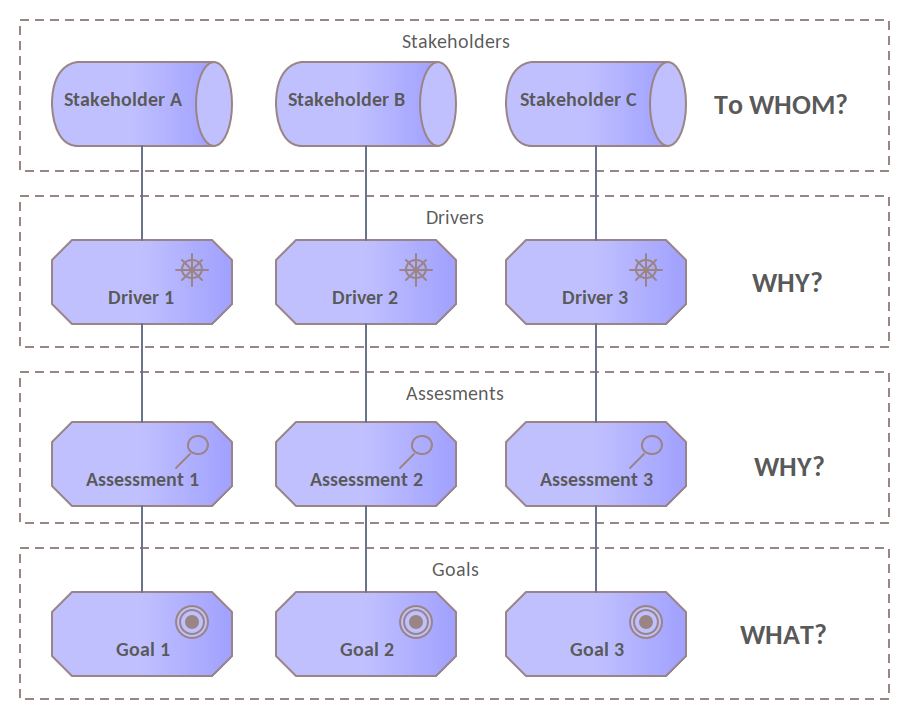
\includegraphics[width=0.7\textwidth]{images/views/Motivation view.png}
		\caption{The layered motivation structure}
		\label{fig:morivation-structure}
	\end{figure}
	
	\textit{Stakeholders} have associated interests, concerns or drivers, which represent internal or external conditions that motivate an organisation to define goals \citep{archimate3.1}.
	
	
	%	\begin{wrapfigure}{r}{0.65\textwidth}
	%		\centering
	%		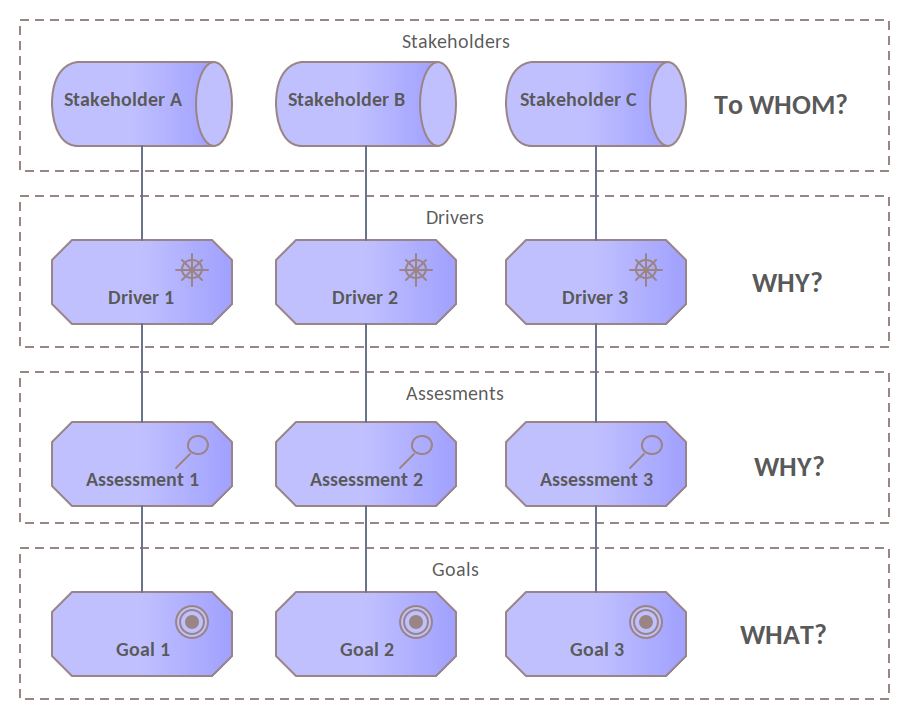
\includegraphics[width=0.67\textwidth]{images/views/Motivation view.png}
	%		\caption{The layered motivation structure}
	%	\end{wrapfigure}
	 
	\textit{Assessments} represent results of analysis of the state of affairs with respect to a driver. They reveal strengths and weaknesses, opportunities or threats to an area of interest \citep{archimate3.1}.
	
	Assessments are associated with goals which represent a high-level statement of intent, plus direction to desired end state for an organisation and its stakeholders \citep{archimate3.1}. 
	
	Next we present the SU motivation structure spread over several sections.
	
	\section{Stakeholders and their roles}
	
	The Standardisation Unit involves multiple stakeholders. We could enumerate them; however, the list would  be long and is outside the scope of this exercise. Instead, we highlight the most important ones and, in addition, we group them based on the role they play in interaction with SU. In Figure \ref{fig:stakehodlers-roles} the roles are depicted as aggregate stakeholders in a grouping frame in the middle of the figure. Above the roles are positioned the most important external stakeholders, while below the stakeholders from the PO are enumerated.
	
	\begin{figure}[!h]
		\centering
		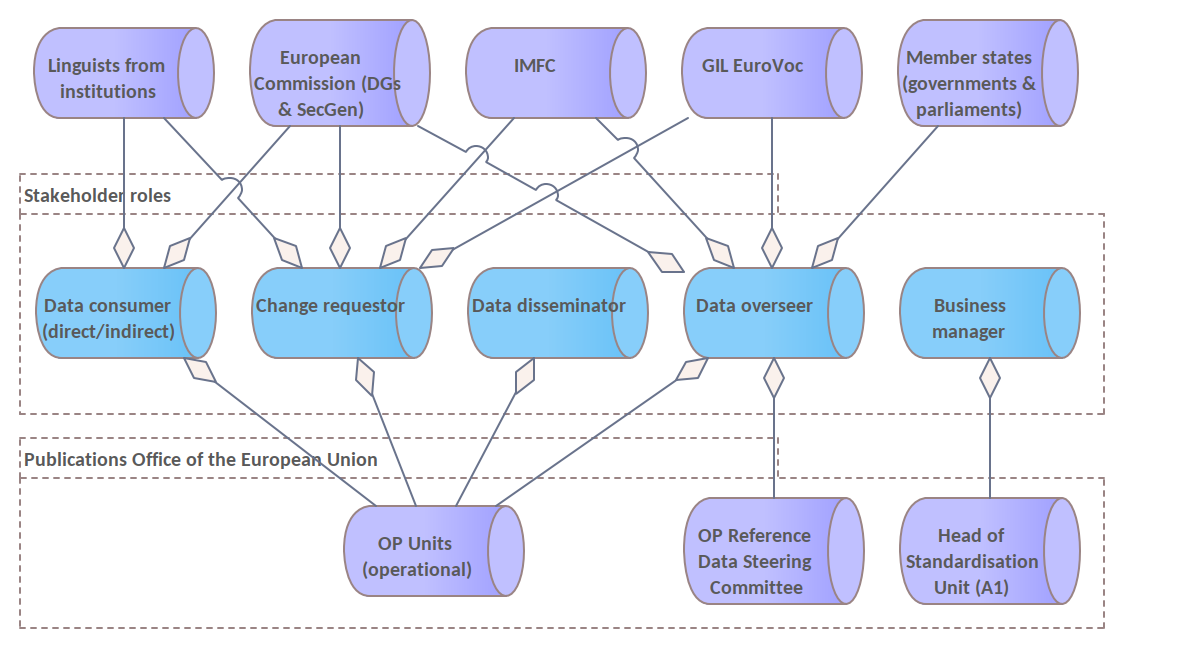
\includegraphics[width=0.8\textwidth]{images/motivation/Stakeholders & Roles.png}
		\caption{The layered motivation structure}
		\label{fig:stakehodlers-roles}
	\end{figure}
	
	The most important external stakeholders are: the European Commission, together with the Secretary General and all of the Commission’s Directorates, the Inter-institutional Metadata and Formats committee (IMFC), Interinstitutional Metadata Maintenance Committee (IMMC), the EuroVoc Committee (Group inter-institutional Lex (GIL)-subgroup EuroVoc), EU Member States (MS) represented by their governments and parliaments, and linguists from different institutions and with a particular interest to the IATE project.
	 
	In Figure \ref{fig:stakehodlers-roles}, the OP stakeholders are placed in organisation-bound context, as the SU is a part of the PO and so its sibling units are not entirely external but are members of the same organisation. The stakeholders within the PO are the various units that use the reference data (e.g. Cellar team, OP Portal team, EurLex team etc.). A Reference Data Steering Committee is scheduled to be formed in the near future in order to coordinate and harmonise the published reference data. And, finally, the Head of the Standardisation Unit (SU) who is in charge of running the enterprise, is also a stakeholder.
	 
	In order to more easily account for the stakeholders' drivers, interests and goals, we grouped them based on their roles in interaction with SU. In Figure \ref{fig:stakehodlers-roles}, the roles are depicted as aggregate stakeholders in a grouping frame in the middle of the figure. The roles include: data consumers, data requester, data disseminators, data overseers and business managers. 
	
	Next we describe each of the roles and briefly enumerate the stakeholders.
	 
	The \textit{data consumers} of published assets are actors who directly engage with and use the published assets in their information systems. Consumers are also considered the actors who use software and services that employs the published assets internally. These consumers are called indirect consumers, while the former ones are called direct consumers.
	
	The \textit{change requester} are agents who require particular content to be available as reference data. 
	
	The \textit{data disseminators} are services and platforms where reference assets are published for broad public consumption.
	
	The \textit{data overseers} are agents who ensure that content satisfying business needs is harmonised, coherent and complete. They are also responsible for the content correctness and harmonisation among multiple stakeholders and its usefulness in the broader context of application. Usually the role of data overseers is performed by the standardisation committees, steering committees and data stewards at large.
	
	\section{Drivers: primary}
	
	We have identified four \textit{primary drivers}, three \textit{secondary drivers} and two \textit{internal efficiency drivers}. The distinction between primary and secondary drivers is based on whether the driver is shared, or not, between the external and internal stakeholders (in this case the business management).
	Figure \ref{fig:primary-drivers} depicts the main stakeholders and their concerns, where the business manager, in this case head of the SU, has the same primary concerns as the main stakeholder roles.
	
	\begin{figure}[h]
		\centering
		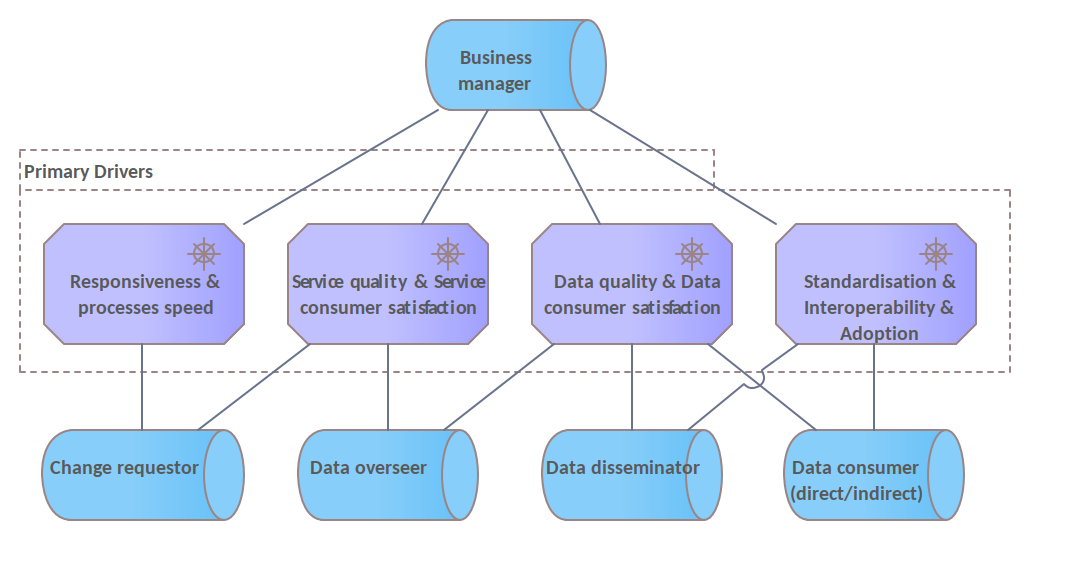
\includegraphics[width=0.9\textwidth]{images/motivation/Primary drivers.png}
		\caption{Primary drivers, motivating both, the internal and external stakeholders}
		\label{fig:primary-drivers}
	\end{figure}
	
	For change requesters, the interaction \textit{responsiveness and the speed of the asset life-cycle process} is of primary concern. The sooner the requests are processed and analysed, the sooner they can be implemented, processed and published. The goal of the SU is to rapidly publish overnight change requests, as compared to the current situation when four major publications are scheduled per year allowing also a few urgent ones in between.
	
	The \textit{quality of service} provided by the SU at large, and service consumer satisfaction, is a direct concern for change requesters and data overseers as primary users of various SU services. 
	
	The \textit{quality of data} is of special interest for data overseers as they are directly responsible for this aspect and implicitly of the data consumer satisfaction. The data quality here has a wide meaning covering aspects of formal, semantic and conceptual correctness while also being timely and up-to-date with the business. Besides data overseers, the data users are also interested in high-quality reference data. Data disseminators are indirectly affected by the quality of the data they distribute and also share this interest to a lesser degree. 
	
	The last of the primary drivers is \textit{standardisation, interoperability and adoption}, which is a major concern for data disseminators and data users. This driver covers the adoption of widely-used meta-models, formally well-defined models representing shared conceptualisation of major bodies and organisations, usage and implementation of national and international standards proposed by standardisation bodies (e.g. ISO, W3C, OMG). These standards refer not only to aspects of data representation, but also to protocols, exchange schemes, validation mechanisms and other tools facilitating systemic interoperability. 
	
	\section{Drivers: secondary}
	The secondary drivers are those that are important to both external and internal stakeholders. They are depicted in Figure \ref{fig:secondary drivers}.

	\textit{Steady and uninterrupted IT systems} is a critical driver for the data consumers. Several institutions and OP units have built IT systems which rely on data maintained and published by the SU. Also, this is one dimension of client satisfaction. The SU ensures that data modifications have no impact on external systems, and for that a part of the life-cycle process is dedicated to impact assessment. 
	
	\begin{figure}[h]
		\centering
		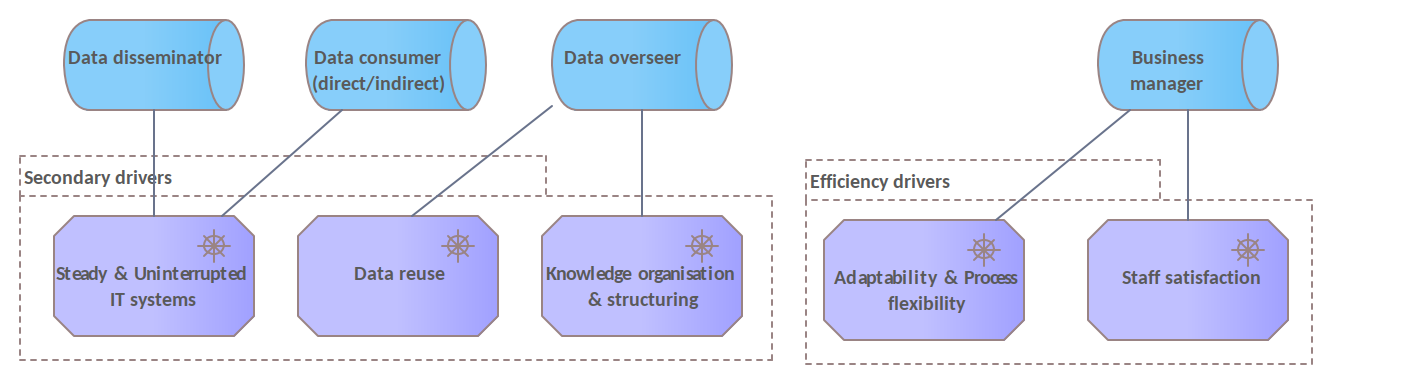
\includegraphics[width=1.05\textwidth]{images/motivation/Secondary drivers.png}
		\caption{Secondary drivers, motivating either internal or external stakeholders}
		\label{fig:secondary drivers}
	\end{figure}
	
	\textit{Data reuse} is encouraged at the level of all EU institutions as a means to reduce integration and development costs. The standardisation committees and other responsible parties (the data overseers) are especially interested in this. 
	
	Keeping the knowledge organisation and its structure in a coherent and consistent form is not a trivial task. Reaching a common shared conceptualisation over a given domain is a goal that is difficult to achieve. Nevertheless, it is a precondition if the data is to be reused by multiple parties. Therefore, this constitutes another driver for data overseers. 
	
	Internally, \textit{staff satisfaction} is an important driver for the SU management. Making sure the business and technical teams can fulfil their duties in a flawless and unhindered manner impacts directly their engagement, satisfaction and productivity.
	
	Requests from external clients sometimes do not lead to data changes alone, but result in changes of the technical processes as well, if not developments of additional processes and components. Adapting and configuring the currently-used process is becoming increasingly difficult; therefore, making sure that these operations are possible with minimal effort and that the production process is flexible, represents a driver for SU management. 
	
	Next we have chosen three drivers we considered to be the most important for this exercise, and we present their assessments. 
	
	\section{Assessment: Responsiveness and processing speed}
	
	A number of causes were identified that decrease responsiveness and process speed. 
	
	\begin{figure}[!h]
		\centering
		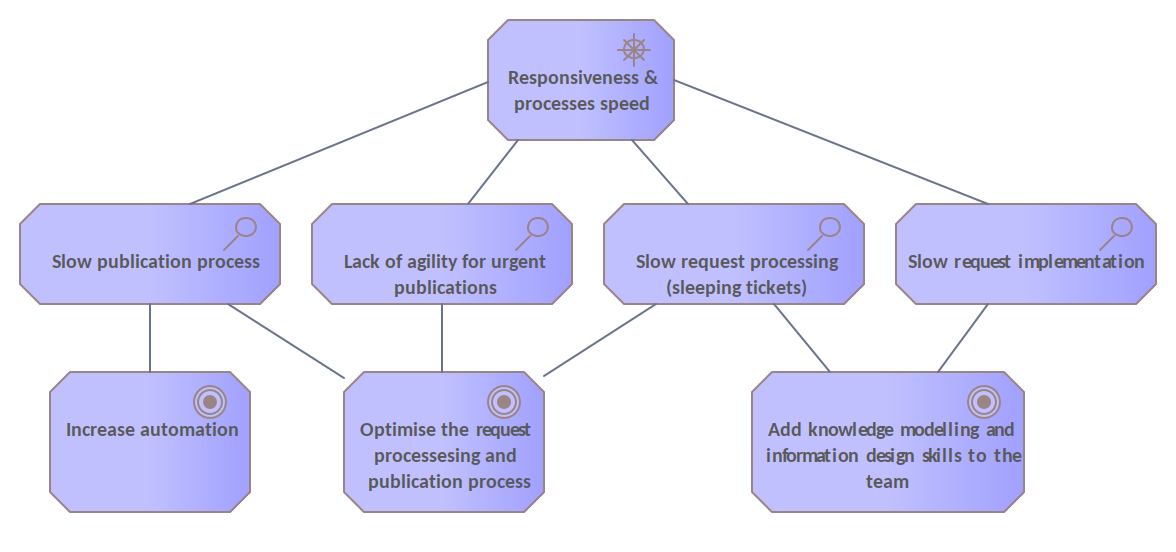
\includegraphics[width=\textwidth]{images/motivation/Responsiveless & Process Speed.png}
		\caption{The assessment of the responsiveness and processing speed driver}
		\label{fig:responsiveness-and-processing-speed}
	\end{figure}
	
	First of all, execution of the entire publication process (including technical and business processes) is slow. This includes burdening by urgent publication requests, which constitute a technical limitation to processing one asset per day. This assessment was provided by the technical team members. 
	
	To address these problems, we aim to increase the automation level which mostly has an impact on technical aspect of the workflow processes. In addition, the increase of automation level is also to optimise the current workflow process, mostly regarding business aspects, in order to reduce the bottlenecks and streamline production.  
	
	In addition, slow processing of change request cases (internally called tickets) is be due to a limit on the number of cases that can be handled by the business team per week. This process becomes even slower when a change request case involves data modelling and design tasks, which sometimes requires consultation with a technical team member or a knowledge organisation engineer. To reduce this bottleneck, training the team to add knowledge modelling skills or recruiting additional staff with such skills are potential solutions.

	\section{Assessment: Data quality}

    Data quality and, implicitly, consumer satisfaction driver have been assessed with the following issues being identified.
    
	\begin{figure}[!h]
		\centering
		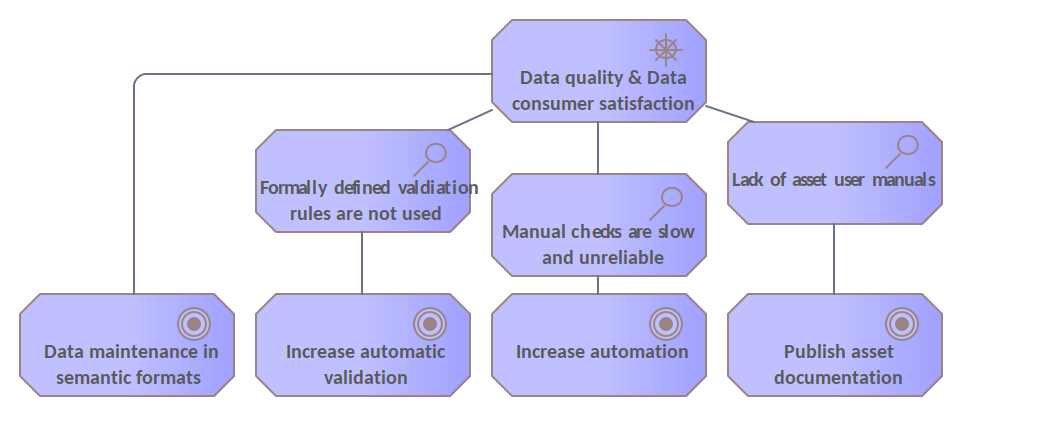
\includegraphics[width=0.9\textwidth]{images/motivation/Data quality.png}
		\caption{The assessment of data quality and data consumer satisfaction}
		\label{fig:data-quality}
	\end{figure}

    The published assets are difficult to adapt by new consumers due to the lack of user manuals. Requests come for both documentation on the conceptual organisation of the asset and the data models used for representing it. We recommend that complete documentation is developed and then published for all assets.
    
    At least for the RDF part of the current publication workflow, the quality assessment is done by technicians undertaking manual checks, ensuring that the transformation processes ran correctly. Therefore, for example, preparing a new version of EuroVoc thesaurus takes days to complete. Moreover, formally-defined validation rules are minimally employed, if at all. The RDF-related processes do not employ SHACL validation, even if the SHACL shape definitions are available. On the XML side, non-semantic validation rules are possible. For these two reasons we propose, as in the previous section, to increase automation and to start employing increasingly more automated validation in order to reduce the time spent by SU team members verifying content before publication. 
    
    Finally, the switch from the XML-based asset sources to RDF-based asset sources is part of the EU trajectory towards public sector linked open data which in turn supports the Public Sector Information (PSI) directive \citep{directive-2019/1024} and the Single Digital Gateway (SDG) initiative \citep{directive-2018/1724}.
    

	\section{Assessment: Service quality}

    A number of complaints have been received, mainly from other OP units, with regards to the quality of services provided by the SU. 

	\begin{figure}[h]
		\centering
		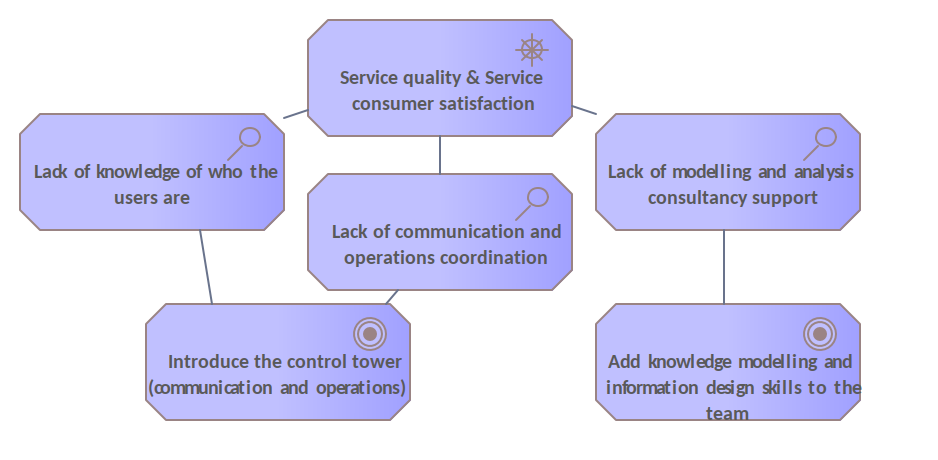
\includegraphics[width=0.8\textwidth]{images/motivation/Service quality.png}
		\caption{The assessment of service quality and service consumer satisfaction}
		\label{fig:service-quality}
	\end{figure}
	
	The complaints are mainly due to the lack of OP internal synchronisation between units, both regarding communication and operational coordination. This is in part linked to a lack of precise knowledge of who the users are and in which manner they engage with assets published by the SU. 
	
	
	To address these two issues, our main recommendation (aligned with SU management vision) is to introduce a control tower-like faculty into the SU, which would take care of synchronisation (communication-wise and operational) with all OP units, and if possible with parties from other institutions and Member States.
	
	Another request often received by the SU is to provide modelling and knowledge organisation services to third party clients: the SU does not currently offer such service. In order to establish the grounds for setting up such service provision in the future, we recommend increasing the number of team members mastering the knowledge modelling and information design domains. 
	
	This brings us to the end of the motivation structure section. While we did not provide an extensive account, we did however identify some SU motivations, drivers and goals that are relevant, directly or indirectly, to the aims of this enterprise architecture.
\section{Business use cases}
\label{sec:business-use cases}
	
	This section presents the core business use cases that have been identified in discussions with SU team members. These use cases have been structured in the light of the new asset life-cycle process, and not the current one, even though they are heavily inspired by the current process. Section \ref{sec:business-architecture} presents the designs of current and new asset life-cycle processes, illustrating both differences and commonalities. The designed processed are derived from the use case descriptions presented below. 
	
	\subsection{UC1: Evolution: Register request for content change}
	\label{sec:uc1}
	
	\textbf{Trigger:} A request for a content change is received in the functional mailbox.
	
	\textbf{Success guarantee:} A complete and clear change request case is created and scheduled for approval.
	
	\textbf{Main success scenario:}
	
	\begin{enumerate}
		\item The client requests a change of one or multiple concepts in an asset
		\item The request manager creates a new change request case and acknowledges the client
		\item The asset manager analyses the request (in terms of business needs and data management implications) and summarises the case
		\item The request manager informs the client of the case summary
		\item The request manager proposes the case for discussion in the next meeting of the team steering committee		
	\end{enumerate}
	\textbf{Extensions:}
	\begin{enumerate}
		\item [4a] The request is incomplete or unclear:
		\begin{enumerate}
			\item [4a1] The asset manager formulates the information requirements			
			\item [4a2] The request manager collects the required details and clarifications from the client
			\item [4a3] Return to step 3 
		\end{enumerate}
		\item [4b] The request is complex and needs deeper conceptual analysis and modelling/design:
		\begin{enumerate}
			\item [4b1] The asset manager presents the case to the knowledge modelling expert 
			\item [4b2] The knowledge modelling expert analyses the case and proposes a solution
			\item [4b3] Return to step 3			
		\end{enumerate}
	\end{enumerate}
	
	
	\subsection{UC2: Evolution: Register request for content change}
	\label{sec:uc2}
	
	\textbf{Trigger:} A team steering committee meeting takes place 
	
	\textbf{Preconditions:} A case is on the meeting agenda 
	
	\textbf{Success guarantee:} The case is rejected or approved for implementation
	
	\textbf{Main success scenario:}
	
	\begin{enumerate}
		\item Any time between when the case is proposed for discussion and the meeting, committee members may assess open cases and add business-, technical- or implementation-related comments. 
		\item During the meeting, the asset manager presents the case.
		\item The steering committee members discuss and comment on the case
		\item The steering committee approves the case for implementation
		\item The asset manager schedules the case for implementation		
	\end{enumerate}
	\textbf{Extensions:}
	\begin{enumerate}
		\item [4a] The case is rejected:
		\begin{enumerate}
			\item [4a1] The steering committee rejects the case along with a justification
			\item [4a2] The request manager informs the client and provides recommendations			
		\end{enumerate}
		\item [4b] The case needs additional input:
		\begin{enumerate}
			\item [4b1]  The steering committee rejects the case along with a request for action, information or agreement for an alternative proposal
			\item [4b2] The request manager informs the user and requests additional actions, information or agreement for an alternative proposal
			\item [4b3] The request manager registers a request for content change (UC1)
		\end{enumerate}
	\end{enumerate}

	\subsection{UC3: Implementation: Implement request for content change}
	\label{sec:uc3}
	
	\textbf{Trigger:} A case is scheduled for implementation
	
	\textbf{Preconditions:} The case is approved for implementation
	
	\textbf{Success guarantee:} The case is implemented and validated, while the data is exported and stored in a common repository
	
	\textbf{Main success scenario:}
	
	\begin{enumerate}
		\item The request manager schedules a case for implementation
		\item The data authoring officer reads the case and executes the content authoring accordingly
		\item The data authoring officer automatically, or assisted by the data processing officer:
		\begin{enumerate}
			\item exports the asset from the authoring tool, and 
			\item runs the SHACL validation for conceptual and structural issues, and
			\item runs the difference calculation between exported content and the previous release export, and
			\item runs the fingerprint calculation for the exported content
			\item the data and reports are stored in the common repository 
		\end{enumerate}		
		\item The data authoring officer checks: 
		\begin{enumerate}
			\item (verification) that the diff report calculated between the previous release export corresponds with the implemented change request\footnote{This is to validate that the export reflects change request case for the change request ticket, keeping the editors on the safe side. If all is good, then this is the final diff.}.
			\item (validation) that no structural anomalies are present in the fingerprint and validation reports.
		\end{enumerate}		 
		\item Repeat steps 1 - 4 until all cases are implemented for the asset
		\item The data authoring officer informs the quality assurance officer of the successful implementation of all cases.		
	\end{enumerate}
	
	\textbf{Extensions:}
	\begin{enumerate}
		\item [2a] Translations are necessary:
		\begin{enumerate}
			\item [2a1] Additionally, the data authoring officer manages the necessary translations and proof-reading (the process is described elsewhere: export selected data for translators, send to the translation unit, import updated data containing the translations, validate and proofread the translations)			
		\end{enumerate}
		\item [4a] Implementation or data is invalid:
		\begin{enumerate}
			\item [4a1] The data authoring officer collects and documents all issues 
			\item [4a2] Return to step 2			
		\end{enumerate}
	\end{enumerate}
	
	\subsection{UC4: Validation: Validate the request for change}
	\label{sec:uc4}
	
	\textbf{Trigger:} An implementation is scheduled for validation (data available in SRC-AP format along with assessment reports)
	
	\textbf{Preconditions:} All cases are implemented for an asset and no further updates are foreseen
	
	\textbf{Success guarantee:} The data is validated by a second "pair of eyes" and is marked as fit for publication
	
	\textbf{Main success scenario:} 
	
	\begin{enumerate}
		\item The data authoring officer provides the data and validation reports in the common repository 
		\item The quality assurance officer verifies that the diff report corresponds to the case requirements
		\item The quality assurance officer checks the fingerprint and validation reports for semantic or structural anomalies
		\item The quality assurance officer accepts the implementation and the data and informs the asset manager
		\item The asset manager marks the asset as fit for publication.
		
	\end{enumerate}
	
	\textbf{Extensions:}
	
	\begin{enumerate}
		\item [4a] Data quality issues are detected:
		\begin{enumerate}
			\item [4a1] The quality assurance officer identifies  and documents issues in the validation and fingerprint reports and informs the data authoring officer what the issues are and eventually explains how to fix them.
			\item [4a2] The data authoring officer implements the request for change (UC3)			
		\end{enumerate}
		\item [4b] Implementation issues are detected:
		\begin{enumerate}
			\item [4b1] The quality assurance officer identifies and documents issues in the diff report and informs the data authoring officer what the issues are and explains how to fix them.
			\item [4b2] The data authoring officer implements the request for change (UC3)			
		\end{enumerate}
	\end{enumerate}


	\subsection{UC5: Release: Prepare the publication content}
	\label{sec:uc5}
	\textbf{Trigger:} Asset release is requested
	
	\textbf{Preconditions:} 
	\begin{itemize}
		\item The data is conceptually and formally validated (SRC-AP) and its content is fit to be published
		\item A code freeze is declared; no more changes are foreseen
	\end{itemize}
	
	\textbf{Success guarantee:} The data is available in standard (and, where requested, additional) forms and formats.
	
	\textbf{Main success scenario:}
	
	\begin{enumerate}
		\item The asset manager requests a release
		\item The data processing officer starts the transformation processes from SRC-AP form into:
		\begin{enumerate}
			\item Target forms: SKOS-AP-EU/Act/Core
			\item Target formats: RDF/XML, Turtle, JSON-LD
		\end{enumerate}		
		\item The data processing officer runs the fingerprinting and SHACL validation for structural issues and confirms the transformation went well\footnote{This process is automatic and has the purpose of ensuring the transformation process passed correctly, keeping the data processing officers on the safe side.}.
		\item The data processing officer start the transformation processes from SRC-AP/SKOS-AP-EU into required additional forms and formats such as CAT-XML, XSD, Genericode, Excel/CSV, MarcXML, GeoJSON, etc.
		\item The data processing officer places the generated output into the common repository along with the validation reports, and informs the asset manager and the publication officer		
	\end{enumerate}
	
	\textbf{Extensions:}
	\begin{enumerate}
		\item [3a] The validation reports reveal content related issues:
		\begin{enumerate}
			\item [3a1] The data processing officer identifies and documents the issues and reports them to the quality assessment officer
			\item [3a2] The data authoring officer implements the request for change (UC3)
		\end{enumerate}

		\item [3b] The validation reports reveal data-related issues:
		\begin{enumerate}
			\item [3b1] The data processing officer identifies and documents the issues and informs the quality assessment officer
			\item [3b2] The data processing officer fixes the issues due to the transformation process
			\item [3b3] Return to step 2
		\end{enumerate}		
	\end{enumerate}
	

	\subsection{UC6: Publish: Publish a reference data asset}
	\label{sec:uc6}		
	
	\textbf{Trigger:} A publication of selected assets is requested
	
	\textbf{Preconditions:} 
	\begin{enumerate}
		\item The selected assets, validated and converted into all the necessary forms and formats, are available in the common repository
		\item The asset user manual is available in the common repository
		\item Format user manuals are available in the common repository
		\item Asset metadata, both content-related and technical, are available in the common repository
	\end{enumerate}

	\textit{Success guarantee:} The updated assets are accessible on selected dissemination platforms and the broad public is informed about the new publication

	\textit{Main success scenario:} 
	
	\begin{enumerate}
		\item The scheduled publication due date occurs
		\item The publication officer generates the release notes from the diff report that summarises what has changed (in more detail than the impact assessment).
		\item The publication officer generates the publication summary and impact assessment report (having sections customised for each major stakeholder) that presents an overview of the main content changes and if structural changes are included. 
		\item The asset manager checks the release notes and the impact assessment (to ensure that they reflect the change request cases)
		\item The request manager sends the publication summary and impact assessment reports to the stakeholders, to inform them of upcoming changes and to collect any pre-publication feedback.
		\item The publication officer runs the packaging process for each asset (parallel to the impact assessment process) resulting in the generation of: 
		\begin{enumerate}
			\item Additional technical metadata (DCAT, METS, IMMC, etc.)
			\item Packages (ZIP or other) for selected dissemination platforms (Cellar, ODP, Bartoc, Joinup, etc.) that contain all the necessary content, documentation and metadata
		\end{enumerate}
		\item The publication officer tests the integrity/fitness of the generated packages by using the validation mechanisms offered by the dissemination platforms (validators or test dissemination environments)
		\item The request manager receives implicit acceptance of the impact assessment from stakeholders (i.e. no objections were raised within the established deadline) and informs the publication officer that the assets can be uploaded to the dissemination platform(s). 
		\item The publication officer publishes the packages to the dissemination platform, tests that the assets are accessible and informs the asset manager that publication has been successfully completed.
		\item The request manager informs the broad public (including stakeholders) that the publication has been completed.
		
	\end{enumerate}
	
	\subsection{UC7: Publish: Publish a model asset}
	\label{sec:uc7}
		
	\textbf{Trigger:} A publication of selected assets is requested
	
	\textbf{Preconditions:} 
	\begin{itemize}
		\item The selected assets, which were approved and converted into the standard forms and formats, are available in the common repository
		\item The asset user manual is available in the common repository
		\item Format/representation user manuals are available in the common repository
		\item Asset metadata, both content- and technical-related are available in the common repository
	\end{itemize}
	
	\textbf{Success guarantee:} The assets are accessible to the broad public on the selected dissemination platforms
	
	\textbf{Main success scenario:} 
	\begin{enumerate}
		\item The scheduled publication due date occurs
		\item The publication officer automatically generates the release notes which summarise the content of the publication.
		\item The request manager sends the publication summary to inform them of upcoming changes and collect any pre-publication feedback.
		\item The publication officer runs the packaging process for each asset (parallel to the impact assessment process), resulting in the generation of: 
		\begin{enumerate}
		\item Additional technical metadata (DCAT, METS, IMMC, etc.)
		\item Packages (ZIP or other) for selected dissemination platforms (Cellar, IMMC, ODP, Wikidata, Bartoc, Joinup, etc.) that contain all the necessary content, documentation and metadata
		\end{enumerate}
		\item The publication officer tests the integrity/fitness of the generated packages by using validation mechanisms offered by the dissemination platforms (validators or test dissemination environments)
		\item The publication officer publishes the packages to the dissemination platform, tests that the assets are accessible and informs the asset manager that publication has been successfully completed
		\item The request manager informs the broad public (including stakeholders) that the publication has been successfully completed
		
	\end{enumerate}
	
	\textbf{Extensions:}
	\begin{enumerate}
		\item [6a] Packages are rejected by the dissemination system:
		\begin{enumerate}
			\item [6a1] The publication officer contacts the support team of the dissemination system and resolves the issue. 
			\item [6a2] In case the generated package is incorrect, the publication officer corrects the generation processes.
		\end{enumerate}
	\end{enumerate}
	
\section{Business architecture}
\label{sec:business-architecture}
	
	This section covers in its extent the business architecture. The focus falls almost entirely on the bottom layer of the business architecture structure (see Figure \ref{fig:business-structure-protopypical}) describing the internal processes, events and roles answering questions concerning who shall do what and when.
	
	
	We address here both the current organisation and the new organisation of the asset life-cycle process. 
	
	First we establish a baseline representing the current setup and, second, we present how the new processes will look like in the light of digital transformations moving towards goals identified in the motivation structure (Section \ref{sec:motivation-architecture}).
	
	Then we explain the general idea of how the business architecture is structured, and which serves as an interpretation framework for the following diagrams. 	
	
	\subsection{Prototypical business structure}
	
	Following the metaphor of layers presented in the motivation view, the organisation of business structure is also explained in terms of layers. Figure \ref{fig:business-structure-protopypical} depicts three layers with the most important elements of the business structure. 
	
%	\begin{wrapfigure}{r}{0.4\textwidth}
%		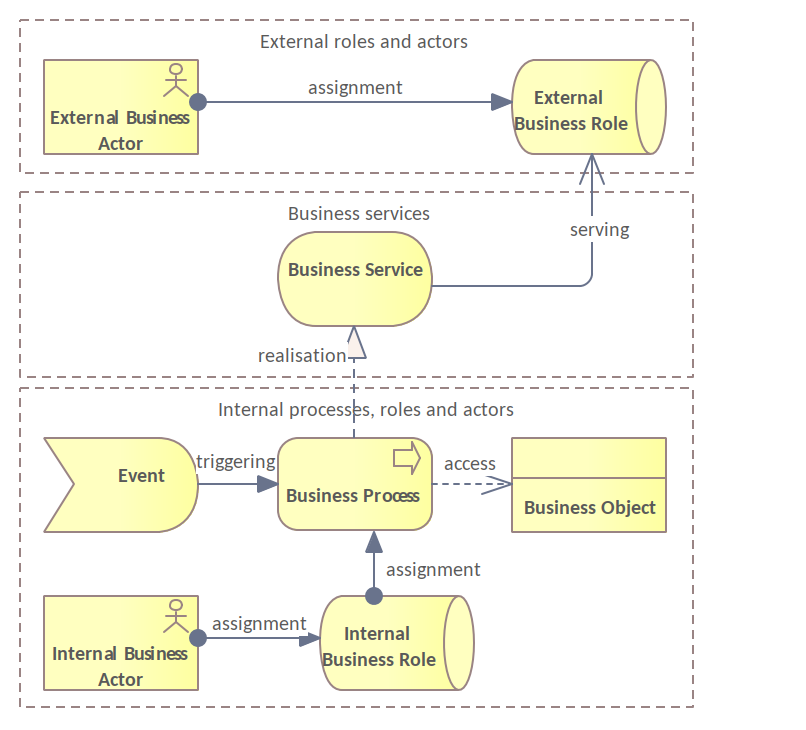
\includegraphics[width=0.4\textwidth]{images/views/Business view.png}
%		\caption{The prototypical business structure view}
%		\label{fig:business-structure-protopypical}
%	\end{wrapfigure}
	
	\begin{figure}[h]
		\centering
		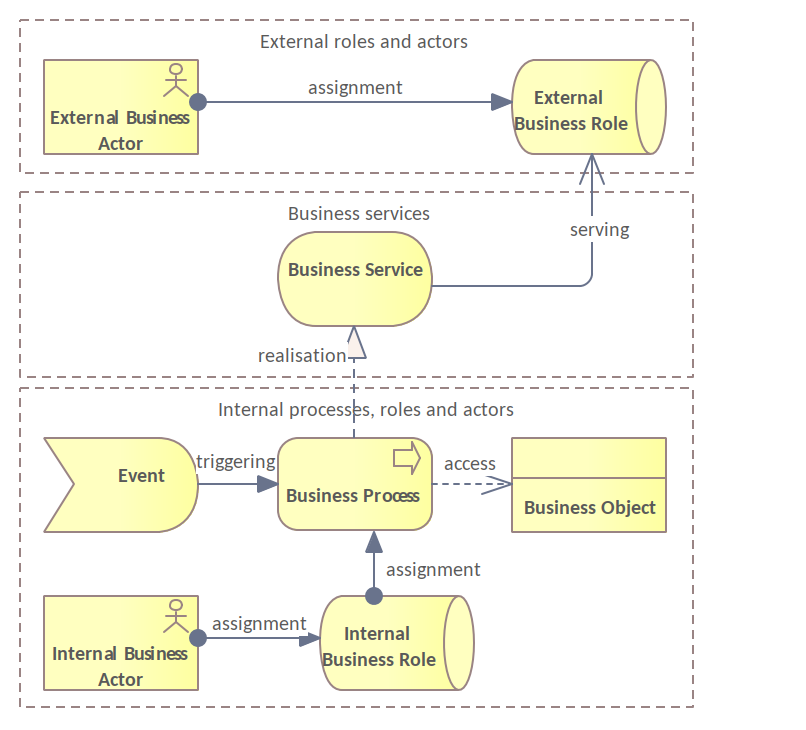
\includegraphics[width=0.4\textwidth]{images/views/Business view.png}
		\caption{The prototypical business structure view}
		\label{fig:business-structure-protopypical}
	\end{figure} 
	
	The topmost layer accounts for the external players or \textit{actors}, which represent a business entity that is capable of performing behaviour and \textit{roles}, which represent skills and responsibilities for performing specific behaviour, and to which an actor can be assigned \citep{archimate3.1}. 
	
	The middle layer represents the \textit{services} that are offered by the organisation to external players. A business service represents explicitly-defined behaviour that a business role, business actor or business collaboration exposes to its environment \citep{archimate3.1}.
	

	
	The lower layers accounts for the internal organisation in terms of \textit{events}, \textit{roles}, \textit{processes} and \textit{objects}. The business process represents a sequence of business behaviours that achieves a specific result such as a defined set of products or business services. The business event represents an organisational state change; while a business object represents a (passive) concept used within a particular business domain.
	

	\subsection{Current asset life-cycle stages}
	\label{sec:lifecycle-current-stages}
	
	The current asset lifec-ycle process is organised in six stages: \textit{inception (or evolution)}, \textit{implementation}, \textit{pre-release}, \textit{release}, \textit{publication} and \textit{consumption}. Each of the stages represents a business sub-process. Figure \ref{fig:lifecycle-current-stages} depicts the order in which stages flow and indicates that each stage process accesses a data asset, the central artefact in the diagram.
	
	\begin{figure}[h]
		\centering
		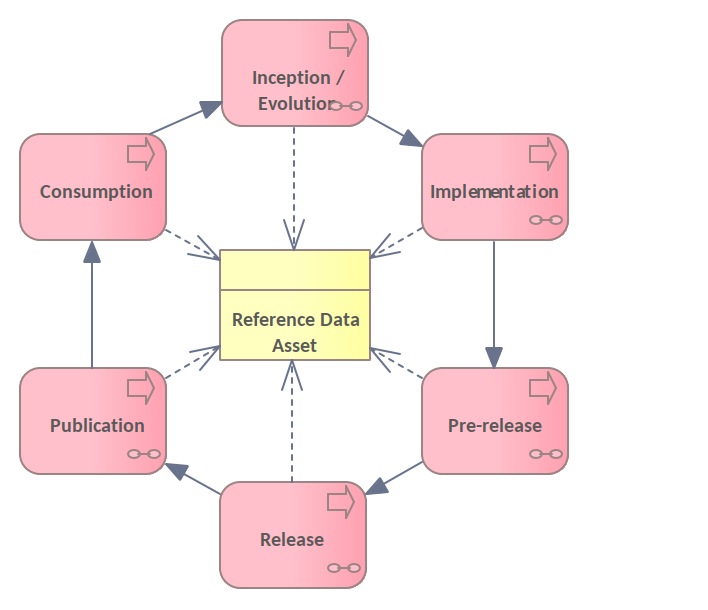
\includegraphics[width=0.5\textwidth]{images/business/Lifecycle process only (current).png}
		\caption{The current asset lifecycle stages}
		\label{fig:lifecycle-current-stages}
	\end{figure} 

	The \textit{inception} stage means that a request arrives for creating and publishing a new data asset and it is being dealt with by the team. The \textit{evolution} stage is similar, only that the request is one for change of an existing data asset. There is no difference in the way these two requests are treated and so the stage name is a conflation of the two. This stage also includes negotiating the request back with the client and then finally deciding and planning its implementation and publication. 
	
	The \textit{implementation} stage deals with actually changing, authoring, converting (MS Excel to XML and back) and verifying the client request. 
	
	\textit{Pre-release} marks that the content has been implemented accordingly and can be validated by a second pair of eyes implementing the \textit{four eyes principle} implemented in SU. This verification and validation is performed by checking the validation reports and by comparing the difference between current and previous versions of the asset conveyed in a diff report. 
	
	In the \textit{release} stage the validated content is placed in a dedicated location of the common repository which indicates that the content is fit for publication. 
	
	The \textit{publication} stage deals with packaging the content and disseminating it to the selected data disseminators, Cellar being the most important. During this stage, a set of announcements and communications ensure that the main stakeholders and the broad public are aware of the published new version of the asset. 
	
	\textit{Consumption} stage is the one that happens outside SU borders. It is clients who use the data and then, in the process, come up with additional requests for either changing existent assets or adding and publishing new ones. 
	
	\subsection{Actors and roles}
	\label{sec:lifecycle-roles}	
	
	This section describes identified actors and roles relevant to the asset life-cycle process. Figure \ref{fig:internal-roles} depicts their relations.
		
	\textit{Asset manager} (a mix of \textit{operational and business data steward}) is primarily responsible for data content, context and associated business rules. This role is characterised by full responsibility for the asset quality, enforcing policies and data governance processes, and ensuring asset fitness (both content and metadata) to business needs. In the SU, this role is also responsible for high-level interaction with main stakeholders and important clients.
	
	\textit{Team steering committee} (also known as the team meetings) is a body composed of business, technical and analytical roles whose main purpose is to provide executive and operational guidance validating business requests and assessing both data management and broader impact, determining implementation priority, as well as promoting data governance and standardisation practices.
	
%	\begin{figure}[h]
%		\centering
%		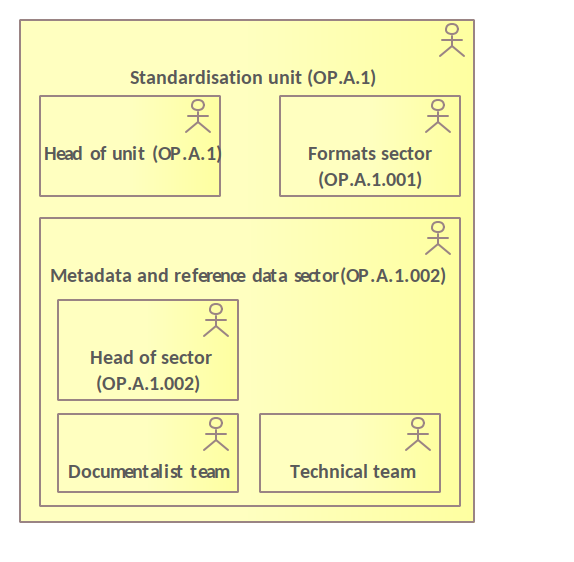
\includegraphics[width=0.47\textwidth]{images/business/Internal Business Actors.png}
%		\caption{The actors in metadata and reference data sector}
%		\label{fig:actors-team}
%	\end{figure} 
	
	\begin{figure}[h]
		\centering
		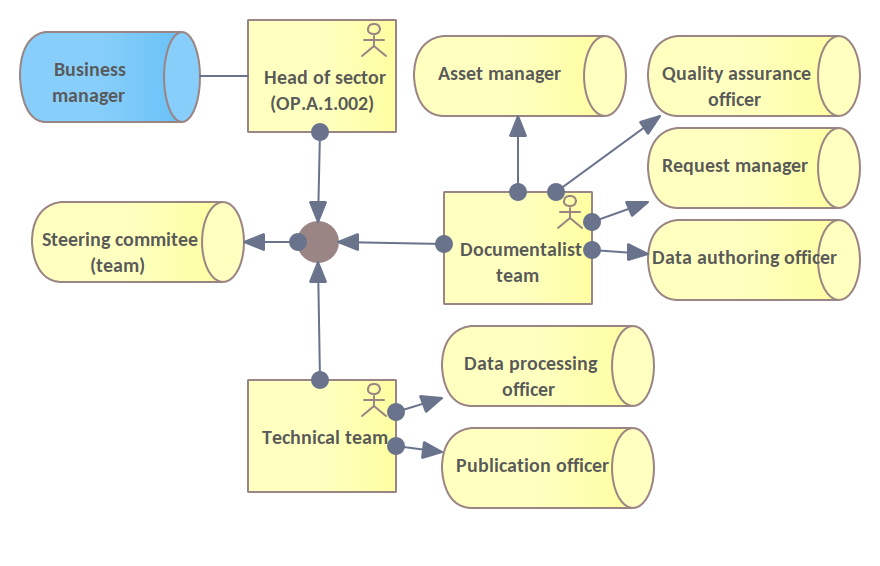
\includegraphics[width=0.7\textwidth]{images/business/Internal Roles.png}
		\caption{The internal roles in metadata and reference data sector}
		\label{fig:internal-roles}
	\end{figure}
	
	\textit{Request manager} is the interface with the client collecting change requests, assessing business needs and translating them into data management requirements, all being summarised and documented case-by-case. 
	
	\textit{Data authoring officer} is responsible for editing data in a content management system implementing the cases prepared by the request manager.
	Quality assurance officers validate that the content implementation is correct from both technical and business points of view. 
	
	\textit{Data processing officer} is a technical role that is responsible for preparing the assets for publication. The responsibilities include, but are not limited to, data storage, manipulation, automatic transformation and generation of validation and assessment reports. 
	
	\textit{Publication officer} is a technical role responsible for packaging and disseminating assets to specialised platforms.
	
	\textit{Stakeholder steering committee} is a body representing the main clients and stakeholders ensuring data and model harmonisation, alignment of data management practices and adoption of international standards.
	
	\textit{Client} (\textit{change requester} and \textit{data user}) is a generic external role who, on one side, consumes data and services provided by the Standardisation Unit and, on the other side, demands publication of new assets or modification of existing ones. 
	
	\textit{Data disseminator} is an external role providing the Standardisation Unit with reliable data dissemination capabilities which are meant to make assets available for clients.

	The external roles and stakeholders have already been addressed in the motivations structure depicted in Figure \ref{fig:stakehodlers-roles}. Each of these roles has a corresponingt element in the business model and will be employed accordingly.

	\subsection{Current asset life-cycle overview}
	\label{sec:lifecycle-current}
	
	This section assembles the asset life-cycle process stages and the main internal roles together into an overview diagram depicted in Figure \ref{fig:lifecycle-current}. It indicates what roles are assigned to which processes, along with a cyclical depiction of the process sequence. Next we comment on the involvement of each role in the asset life-cycle process. All the life-cycle stages are internal to the SU except for the last one, consumption, which takes place at the client's premises.
	
	\begin{figure}[h]
		\centering
		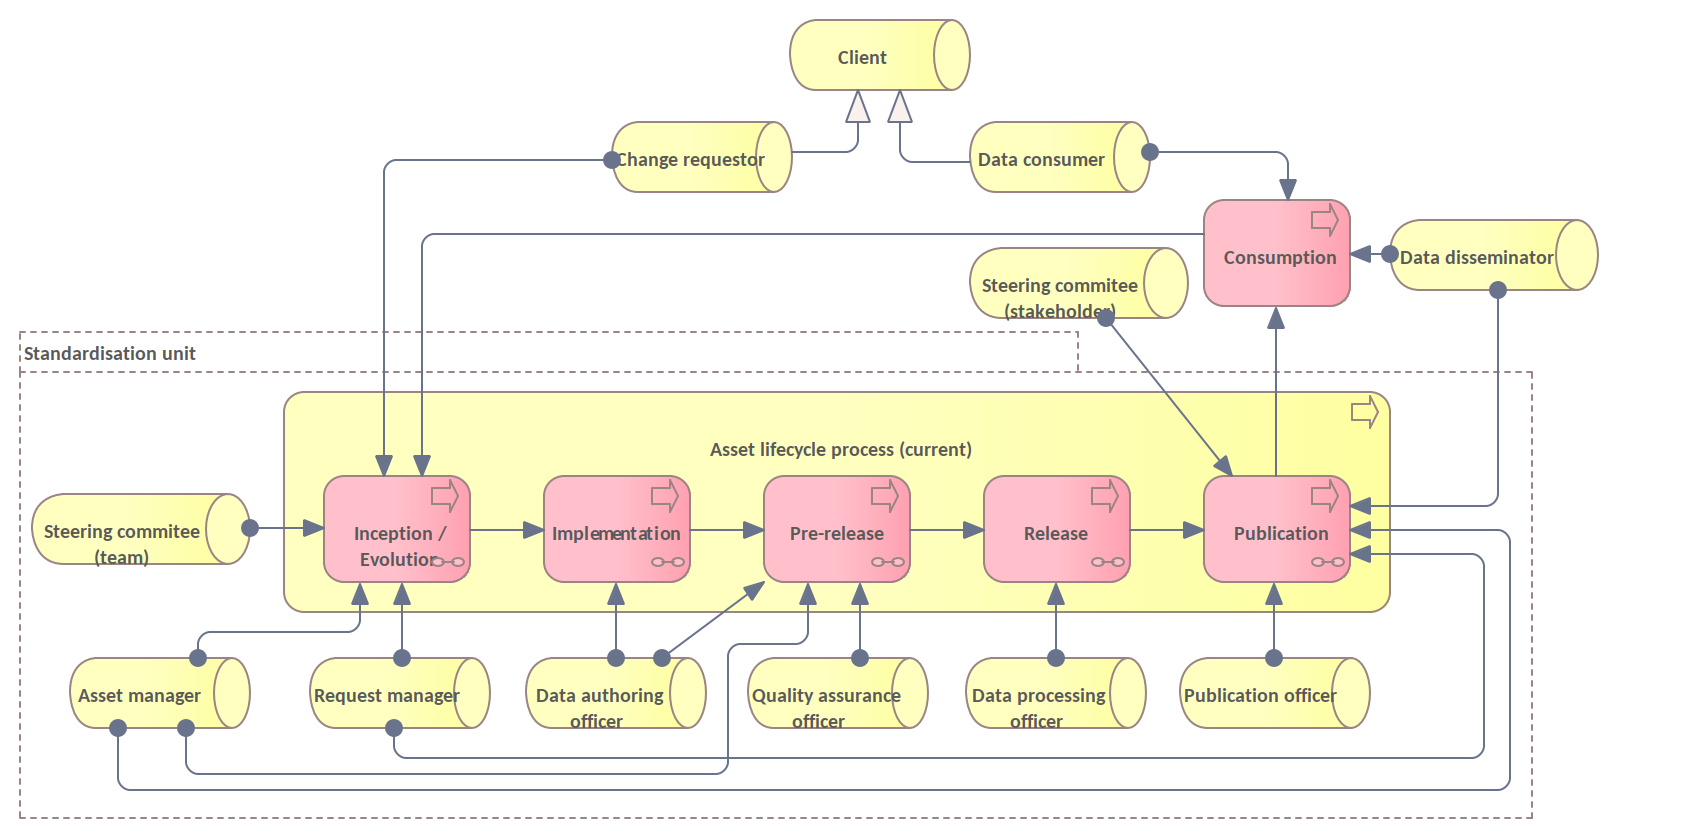
\includegraphics[width=1.05\textwidth]{images/business/Lifecycle (current).png}
		\caption{The current asset lifecycle stages and roles}
		\label{fig:lifecycle-current}
	\end{figure} 
	
	In the inception/evolution stage, the request manager is responsible for creating, documenting and ensuring descriptive completeness for requests arriving from clients to change existent assess or to create of new ones. These requests are managed as individual or, sometimes, interdependent cases. This role serves as the primary interface with the third parties. For this reason, in the publication stage, this role communicates with the stakeholders and broad public about the asset changes when it is published.
	
	The asset manager is in charge of analysing and summarising the request case in the inception/evolution stage. This role intervenes in the pre-release stage to acknowledge that the case has been implemented and the asset is fit for publication; and in the publication stage to check the impact assessment and the release notes before they are used in the communication with external parties.
	
	The team steering committee is involved in the initial stage only. After a new change request case is created, the team steering committee decides whether the case shall be further processed; and if so, then the decision is about when and how.
	
	The data authoring officer is responsible for the case implementation and, in the pre-release stage, verifying and validating its own work as the ``first pair of eyes'' (of the ``two pairs of eyes'' principle). The ``second pair of eyes'' verifying and validating the case implementation is enacted vy the quality assurance officer in the same pre-release stage.
	
	Once the case is marked as fit for publication, in the release stage, it is placed automatically or by intervention of the data processing officer in a region of the common repository tagged for ``release''. If are any technical issues are encountered, the the data processing officers intervenes and fixes them.
	
	
	In the publication stage, the publication officer generates the release artefacts, the release notes, packages the assets and disseminates them to the dissemination partners. External steering committees, such as IMMC metadata sub-committee, GIL EuroVoc an others are asked for final feedback two weeks in advance before the final dissemination.
	
	Next, we turn to discuss the asset lifecycle stages in more detail as elicited from the technical and business teams of the SU. These descriptions are not covering the ultimate details of the process but aim at describing the important building blocks of the current stages. 
	
	\subsection{Current inception and evolution stage}
	\label{sec:inception-current}
	
	\begin{figure}[h]
		\centering
		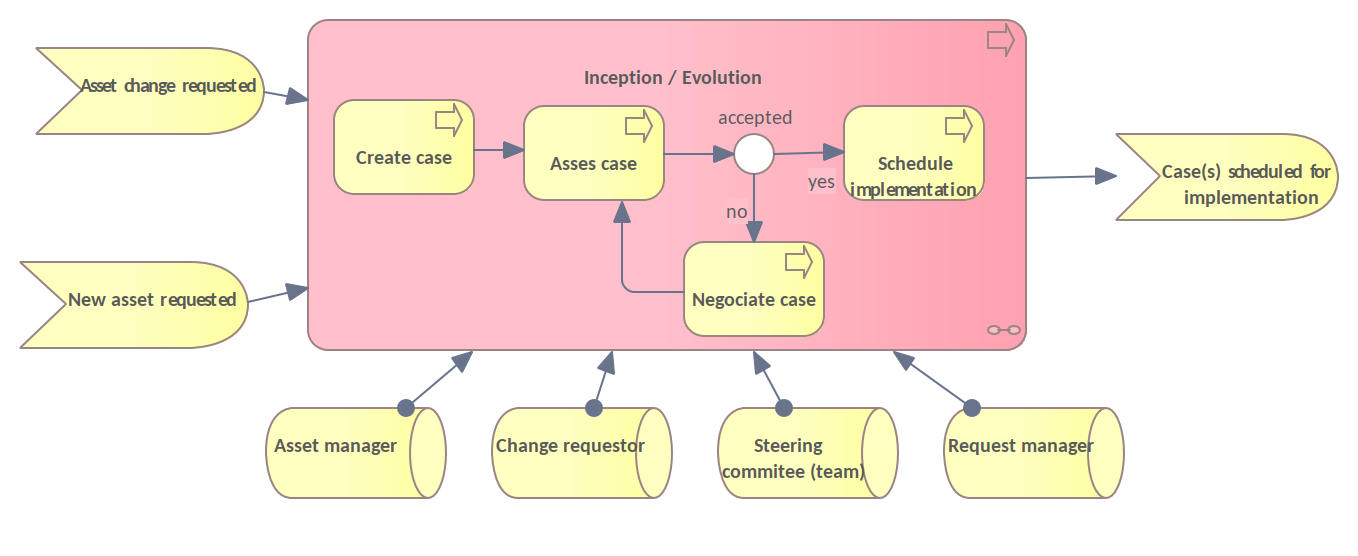
\includegraphics[width=.8\textwidth]{images/business/current/InceptionEvolution.png}
		\caption{The current process for the inception and evolution stage}
		\label{fig:evolution-current}
	\end{figure}		
	
	The process, depicted in Figure \ref{fig:evolution-current}, starts when a request from a client arrives to either update a data asset or create a new one. This case, after being recorded, analysed and summarised, is asses by the asset manager and then discussed in the team meeting. 
	
	
	In case the case is accepted, then it is scheduled for implementation. Otherwise the case enters a so called negotiation stage, due to one of two things being the case: either the case is incomplete and more information is required from the client, either the case is unacceptable and a rejection is provided to the client with an explanation why or eventually with counter proposals. 
	
	The client communication is mainly carried out by email or telephone conversations, whereas the cases are managed using Jira ticket management system \citep{jira}. 
	
	The process ends when the case is rejected or when it is scheduled for implementation. 

	
	\subsection{Current implementation stage}
	\label{sec:implementation-current}
		
	Figure \ref{fig:implementation-current} depicts the current implementation process. It starts, when the case is queued for implementation. The data authoring officer modifies the asset content according to the instructions provided in the case description. The editing takes place in an Microsoft Excel \citep{excel} workbook which represents an interface to the asset content. Excel is the main editing tool. Once the changes are complete, the workbook is committed into SVN repository \citep{svn}, which triggers and automatic conversion of the Excel workbook into an XML form \cite{xml11-spec}. The XML is considered the primary asset source (structured with CAT XSD scheme). It is further converted back into Excel form, this way entering a conversion loop which also serves as validation mechanism ($XML \rightarrow Excel \rightarrow XML \rightarrow Excel$).
	
	\begin{figure}[h]
		\centering
		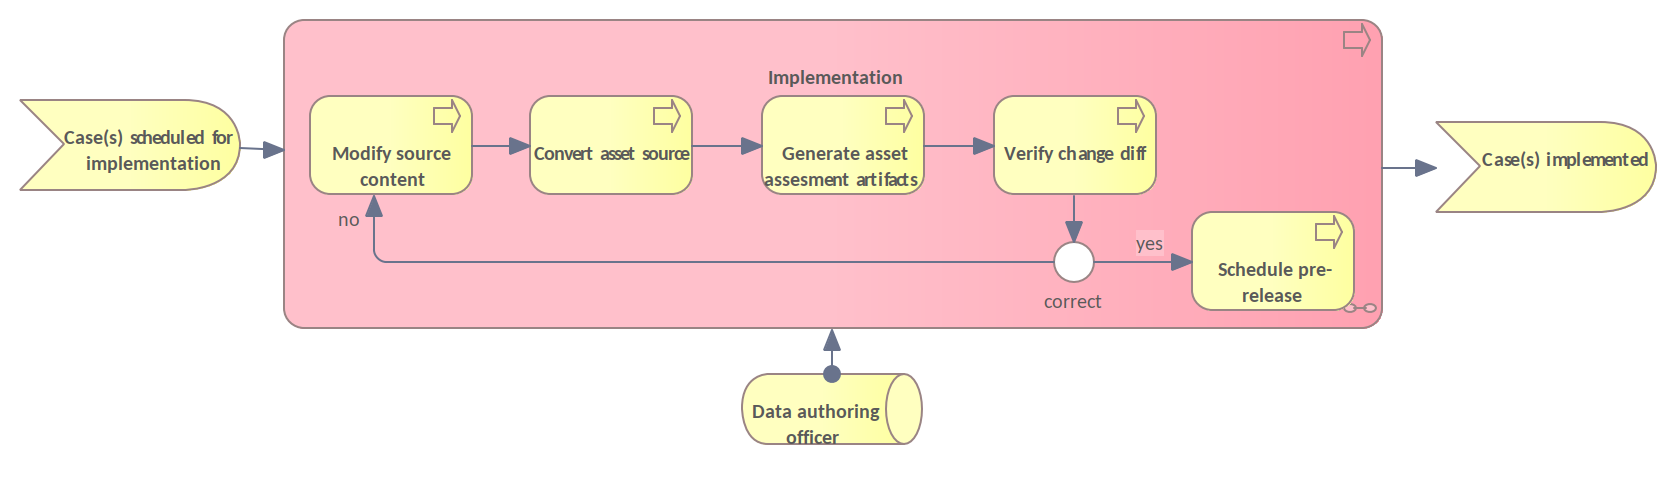
\includegraphics[width=.9\textwidth]{images/business/current/Implementation.png}
		\caption{The current process for the implementation stage}
		\label{fig:implementation-current}
	\end{figure}
	
	Once the asset is converted into XML form, it becomes possible through a set of Perl scripts and XSLT style-sheets \citep{xslt3-Kay} to automatically generate assessment artefacts such as the diff report and schema validation report. The diff report indicates what changes have been done to the content between the previous and the latest version, while the validation report contains violations, if any, of XML structural constraints.
	
	The editor then verifies the diff report to ensure the case implementation completeness and that the asset can be tagged for pre-release. Otherwise the content is being edited again. 
	
	The process end with the asset being marked for pre-release, which means that the case implementation is complete.
	
	\subsection{Current pre-release stage}
	\label{sec:pre-release-current}	

	The pre-release stage is depicted in Figure \ref{fig:pre-release-current}. Once the case is marked as implemented, and the assessment artefacts were generated after the conversion into XML form, the second verification and validation can be performed by the quality assurance officer. 
	
	\begin{figure}[h]
		\centering
		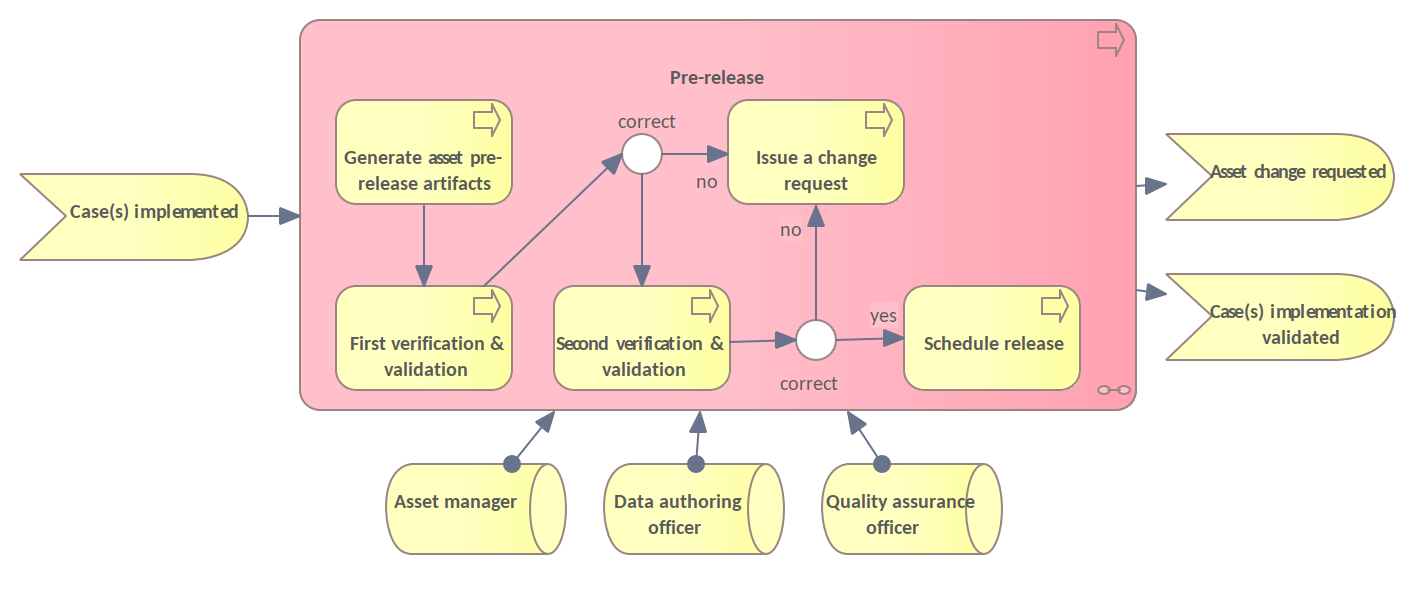
\includegraphics[width=.65\textwidth]{images/business/current/Pre-release.png}
		\caption{The current process for the pre-release stage}
		\label{fig:pre-release-current}
	\end{figure}

	In case issues are identified in the case implementation, the quality assurance officer created a new request for changes and the case returns to the implementation stage, otherwise the case implementation is validated and the asset is marked as ready for release. 
	
	This is process where mostly manual steps are taken. Some minor content transformation can take place such as RDF content prettyification and an additional validation of record identifiers in the XML file. These these operations, however, are merely technicalities and do no have business relevance. Therefore they are omitted in the process diagram from Figure \ref{fig:pre-release-current}. 

	\subsection{Current release stage}
	\label{sec:release-current}
	
	\begin{figure}[h]
		\centering
		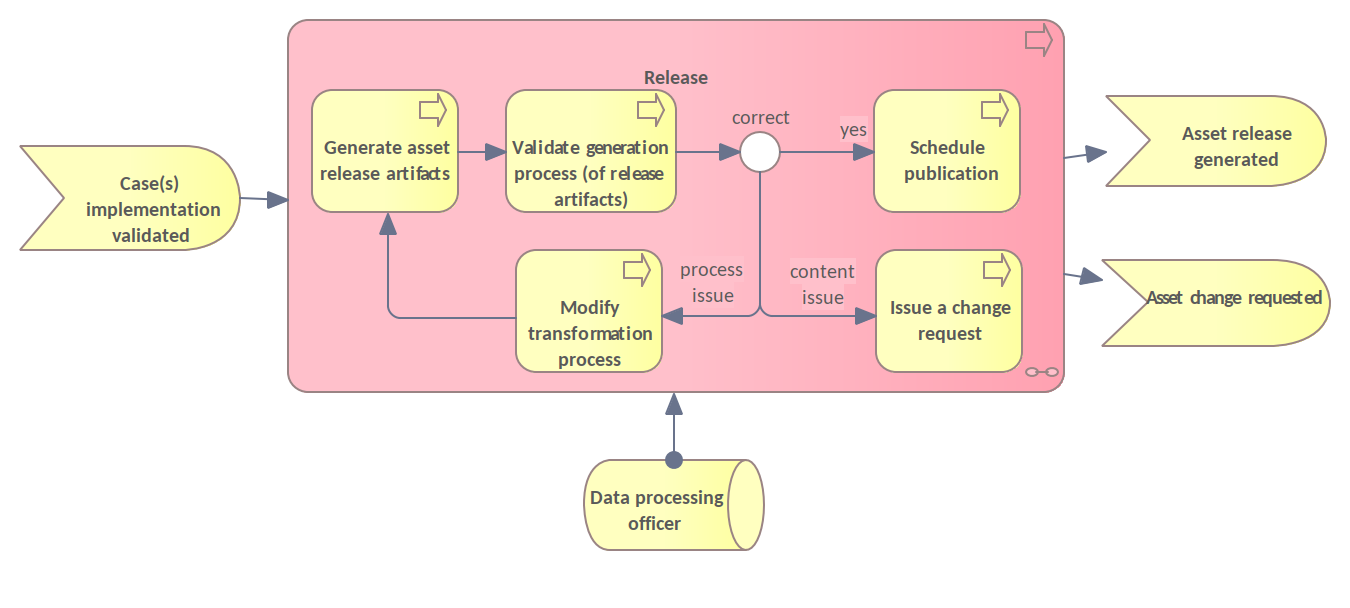
\includegraphics[width=.6\textwidth]{images/business/current/Release.png}
		\caption{The current process for the release stage}
		\label{fig:release-current}
	\end{figure}

	The release stage is a symbolic step where an asset is simply marked as being in the release stage after it has been verified and validated by four pairs of eyes and confirmed that all the cases had been correctly implemented and that the asset is fit for release in the subsequent publication. This si depicted in Figure \ref{fig:release-current}.

	The release stage is realised by copying the updated version of the asset into a special area of the common repository and marked with the ``release'' tag.

	\subsection{Current publication stage}
	
	The current publication stage is depicted in Figure \ref{fig:publication-current}. It is a wide process that involves almost all the multiples roles. 
	
	\label{sec:publication-current}
		\begin{figure}[h]
		\centering
		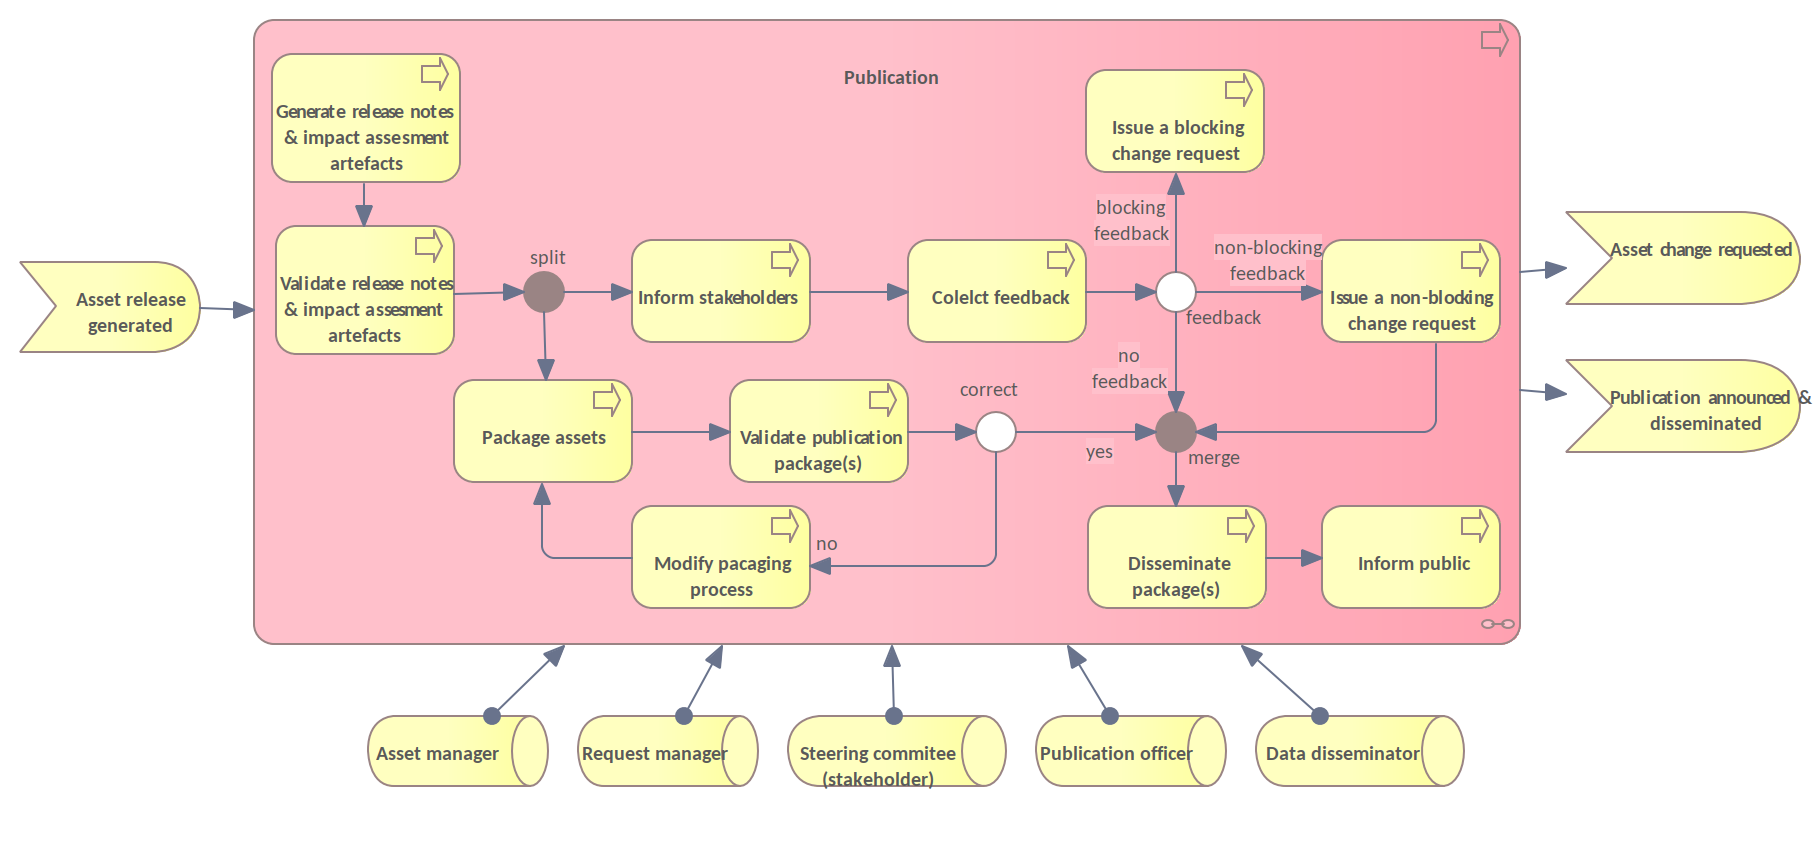
\includegraphics[width=1.03\textwidth]{images/business/current/Publication.png}
		\caption{The current process for the publication stage}
		\label{fig:publication-current}
	\end{figure}

	The publication process starts several weeks before the scheduled publication date, when a code freeze is announced and all the pre-selected assets are marked for release. It commences by generating from the CAT-XML source a selection of forms and formats to ease asset consumption by various clients. Mostly XSD, CAT-XML, SKOS-AP-EU forms are generated that are serialised in XML, Turtle and JSON formats. In addition some assets are also prepared in Genericode, Excel/CSV, MarcXML, GeoJSON and other forms. 
	
	Next, the publication notes are prepared together with a few different impact assessments specially prepared for targeted stakeholders. These communication artefacts are checked for correctness and sent to the corresponding stakeholders. After a predefined number of days (usually two weeks) the feedback is collected, if any. Reception of no feedback is considered as a tacit acceptance of the current publication and the process can continue. Seldom, blocking or non-blocking feedback is received which leads to creation of new change requests, and depending on the situation, last minute changes are executed. Or, if the feedback is non-blocking, the intervention is scheduled or the next publication. 
	
	In parallel a packaging process is executed during which, the assets are prepared for dissemination. They are assembled in packages accompanied by their content-related and technical metadata, user manuals, format documentation and, of course, the asset itself expressed in all pre-generated forms and formats, the release artefacts. The packages are verified whether the target dissemination platforms accept them.
	
	Finally the packages are disseminated and the successful publication is announced to the broad public. The dissemination is done primarily through Cellar\citep{cdm-francesconi2015ontology} although other dissemination channels are also employed, among which Wikidata\citep{vrandevcic2014wikidata}, Publications Office Open Data Portal (ODP), Bartoc \citep{ledl2016describing}, JoinUp platform \citep{hillenius2013free}.
	
	This section completes the detailed presentation of the asset lifecycle process as it is today. 
	
	The digital transformation currently undertaken by SU management, that is in part targeted by this architecture, has impact on the asset lifecycle business, application and technical architectures. The next sections will describe how the new asset lifecycle architecture is envisaged. 
		
	\subsection{New asset lifecycle overview}
	\label{sec:lifecycle-new}	
	
	The structure of the new asset lifecycle process is depicted in Figure \ref{fig:lifecycle-new}. In this new architecture, we aim to propose incremental changes, as to cause least disruptions to the team and the ongoing operations. 

	\begin{figure}[h]
		\centering
		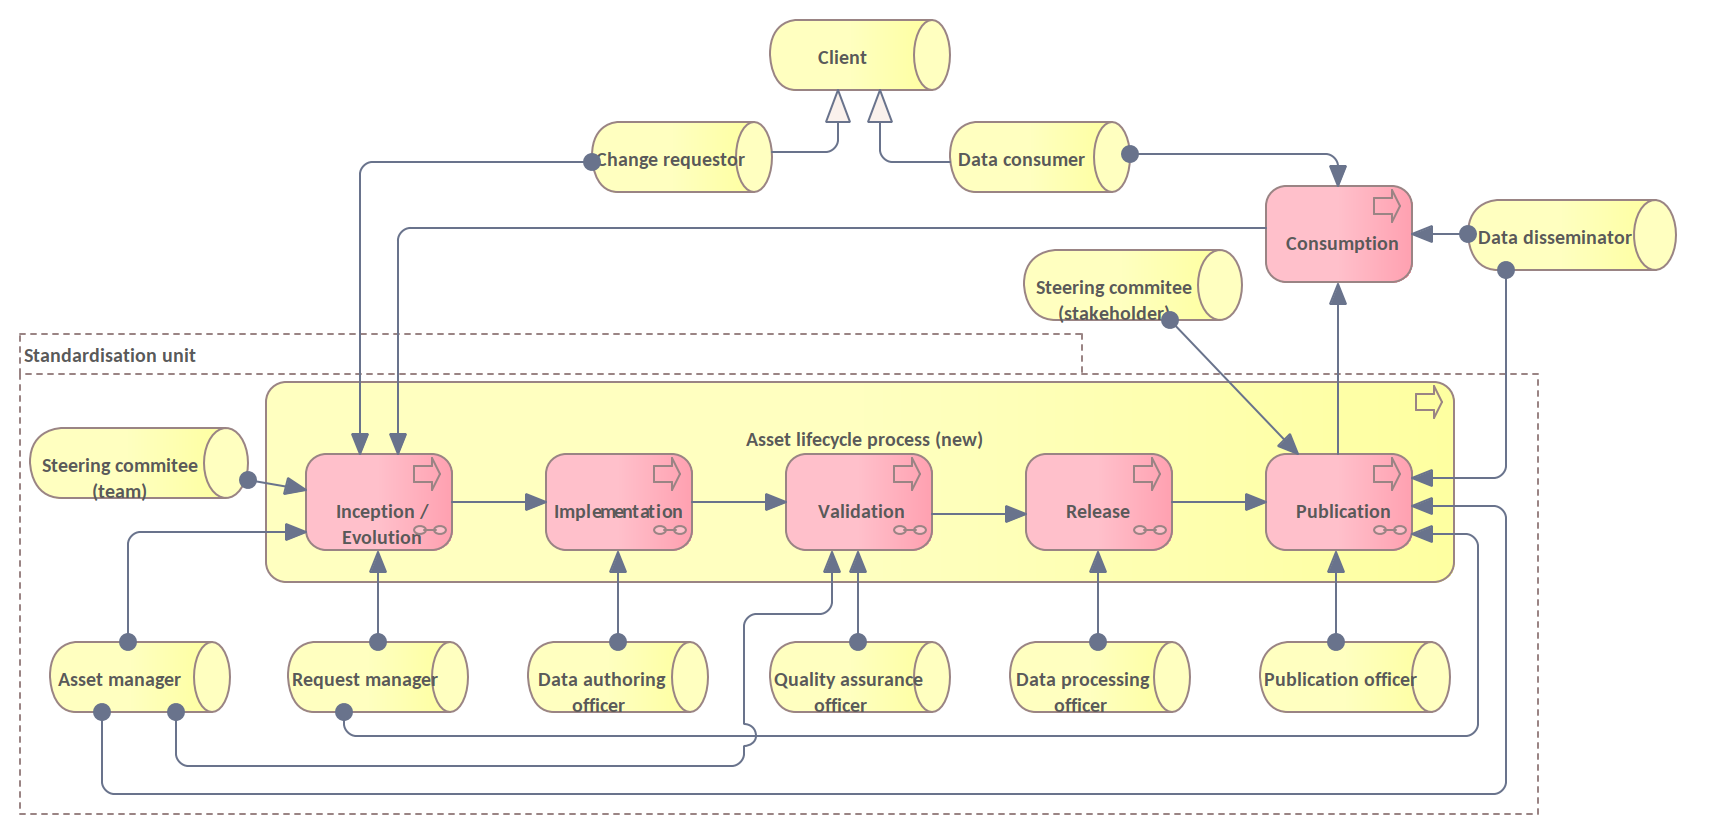
\includegraphics[width=1.05\textwidth]{images/business/Lifecycle (new).png}
		\caption{The current asset lifecycle stages and roles}
		\label{fig:lifecycle-new}
	\end{figure}
	
	This process is similar, in its structure and stage names, to the current one: six stages circularly linked. The only change is the replacement of pre-release stage a stage called validation. There are however significant changes in the structure of three stages: implementation, validation and release, while the inception/evolution stage is identical to the current one, and the publication stage are is almost entirely unchanged. These changes are addressed in detail in the next sections.
		
	There are no new roles in the new process, but there is a difference in the role allocation and involvement at different stages of the process as compared to the current one. 
	
	As mentioned above, the implementation/evolution stage is identical to the current one. So after the case has been registered and processed the implementation is scheduled. How it happens in the new workflow is presented in the next section. 
			
	\subsection{New implementation stage}
	\label{sec:implementation-new}

	The new implementation process is depicted in Figure \ref{fig:validation-new}. The main digital transformation at this stage is adoption of RDF asset source, and the switch from Microsoft Excel as the content editor to VocBench3 \citep{stellato2017towards,stellatovocbench} semantic web editor. 
	
	\begin{figure}[h]
		\centering
		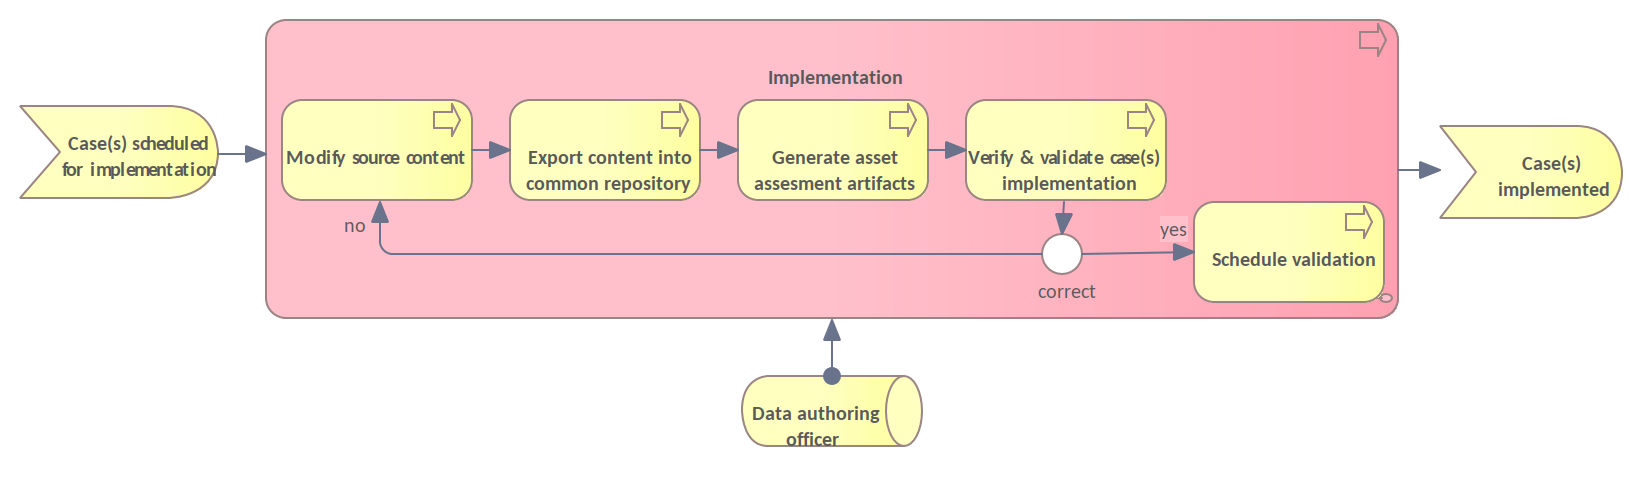
\includegraphics[width=1.05\textwidth]{images/business/new/Implementation.png}
		\caption{The new process for the implementation stage}
		\label{fig:implementation-new}
	\end{figure} 

	The overall process looks very similar to the current one, but the employed technology for the source editing: VocBench3 and SKOS model(s) \citep{skos-spec}, render an entirely different editor experience when modifying the source content to implement the request case.
	
	When the editing is complete, the content is exported from VocBench into the common repository and a set of asset assessment artefacts are generated. These artefacts are: the asset diff report, the fingerprint report and the validation report (based on SHACL \citep{shacl-spec} validation rules). These reports are no longer implemented based on the XSLT technology \citep{xslt3-Kay}, because the underlying source is the new RDF representation \citep{rdf11} and no longer (CAT-)XML. More technical details are addressed in the application architecture in Section \ref{sec:implementation-application}.
	
	The editor (data authoring officer) then verifies that the case is implemented correctly, and if so a validation, by the quality assurance office is scheduled, otherwise, if some issues are spotted more editing is performed in VocBench3.
		
	
	\subsection{New validation stage}
	\label{sec:validation-new}	
	
	The validation stage is new in the asset lifecycle process. Here the correctness assessment is separated into two steps: verification and validation. This is a continuation of the current conception of how the case implementation is being assessed. The verification is primarily focused on the business aspects of the case implementation; whereas, the validation, deals with the technical and more formal aspects of the content structure and consistency. As the new technology allows for semantic accounts, then validation extends to deal with semantics as well. 	 

	\begin{figure}[h]
		\centering
		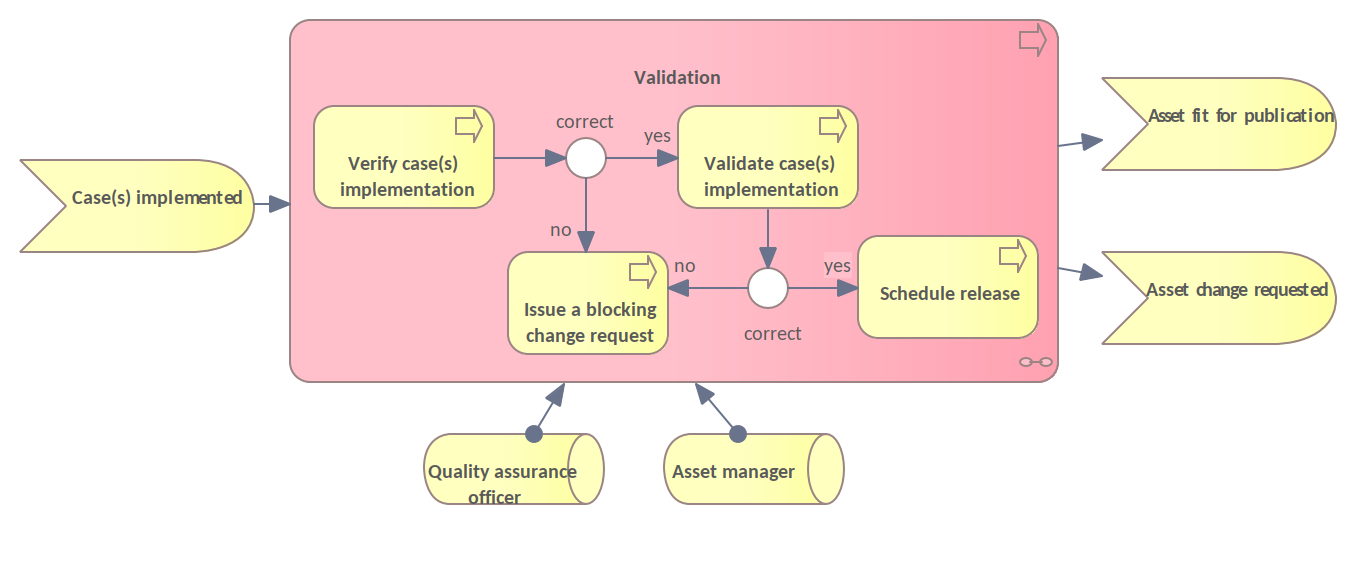
\includegraphics[width=.892\textwidth]{images/business/new/Validation.png}
		\caption{The new process for the validation stage}
		\label{fig:validation-new}
	\end{figure}

	In case errors are detected in the implementation, the quality assurance officer issues a  change request and the case goes back into the implementation stage. Otherwise, the case implementation is considered correct and from now on a release can be scheduled. This is performed by the asset manager. 
		
	\subsection{New release stage}
	\label{sec:release-new}
	
	The new release stage, depicted in Figure \ref{fig:release-new}, differs considerably from the current one. This stage is no longer one of simply marking the asset implementation as fit for publication but deals with all the data transformations and preparation of artefacts necessary in the publication stage.
	
	\begin{figure}[h]
		\centering
		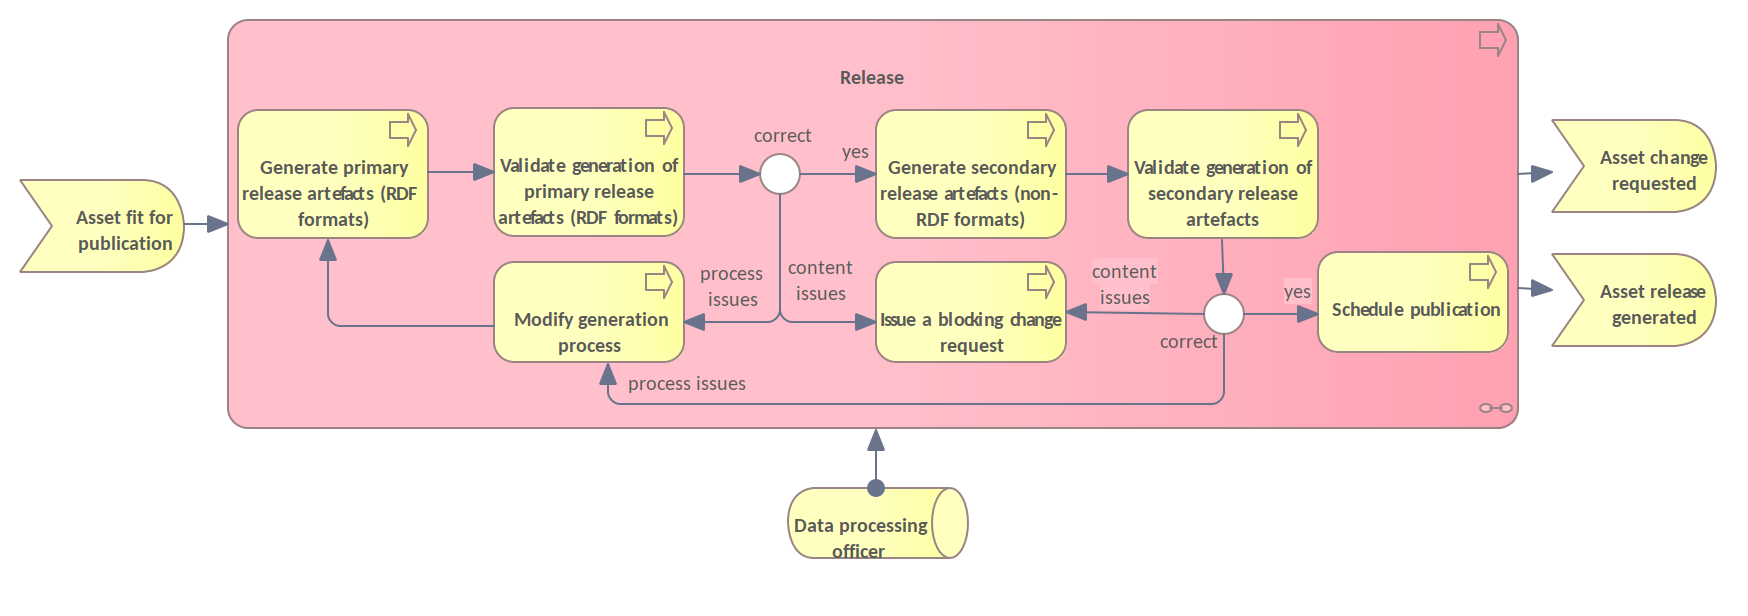
\includegraphics[width=1.05\textwidth]{images/business/new/Release.png}
		\caption{The new process for the release stage}
		\label{fig:release-new}
	\end{figure}

	The release starts when all the change request cases, in the scope of the scheduled publication, have been implemented and validated. Then, the primary release artefacts are generated from the RDF source expressed in SRC-AP form \citep{src-ap-vb3}. The main artefacts are the source in SKOS-AP-EU form \citep{skos-ap-eu}, a special extension of the SKOS-AP-EU which is necessary for publishing the content in Cellar because of the backwards compatibility issues (called SKOS-AP-EU-Act), and the SKOS core \citep{skos-spec} representation. These artefacts are also generated in RDF/XML \citep{rdf-xml-Schreiber:14:RXS,rdf-xml-Beckett:04:RSS}, Turtle \citep{turtle-Carothers:14:RT} and JSON-LD \citep{sporny2014json,spornyjson} formats. 
	
	The transformation process is accompanied by a set of validation processes meant to safeguard the and ensure that the transformations are executed correctly. The validation reports are checked by the data processing officer. In case process related issues are detected, then most likely the processes contain bugs and need to be fixed. In case content related issues is spotted then a new change request is created and the process goes back to the implementation stage. 
	
	After the primary release artefacts are created, then secondary release artefacts are created. All of them are non-RDF forms and formats that currently are produced for clients (CAT-XML, XSD, Genericode, Excel/CSV, MarcXML, GeoJSON, etc.) and must continue so. An automated validation of the generated assets, to the extent possible, secures and ensures quality of the output. Like in the case of the primary artefacts, if the errors are detected then depending on their nature, either the data transformation process must be updated or a content change request is issued and the process returns back to the implementation stage. 
	
	The transformation technology employed here needs to provide ETL\footnote{Extract, transform, load (ETL) is the general procedure of copying data from one or more sources into a destination system which represents the data differently from the source(s) or in a different context than the source(s).}/ELT\footnote{Extract, load, transform (ELT) is a variant of ETL where the extracted data is loaded into the target system first.}-like capabilities for both: RDF and for data formats. An extended discussion about the application capabilities is covered in Section \ref{sec:release-application}.
	
	At the end of this stage, all the important asset transformations and data conversions must be complete and the necessary forms and formats consumed by target clients shall be available for publication. Finally the assets are copied into the special place of the common repository available to the publication process. 
	
	\subsection{New publication stage}
	\label{sec:publication-new}
	
	The new publication stage process is depicted in Figure \ref{fig:publication-new}. This process is very similar to the one currently performed described in Section \ref{sec:publication-current}.
	
	\begin{figure}[h]
		\centering
		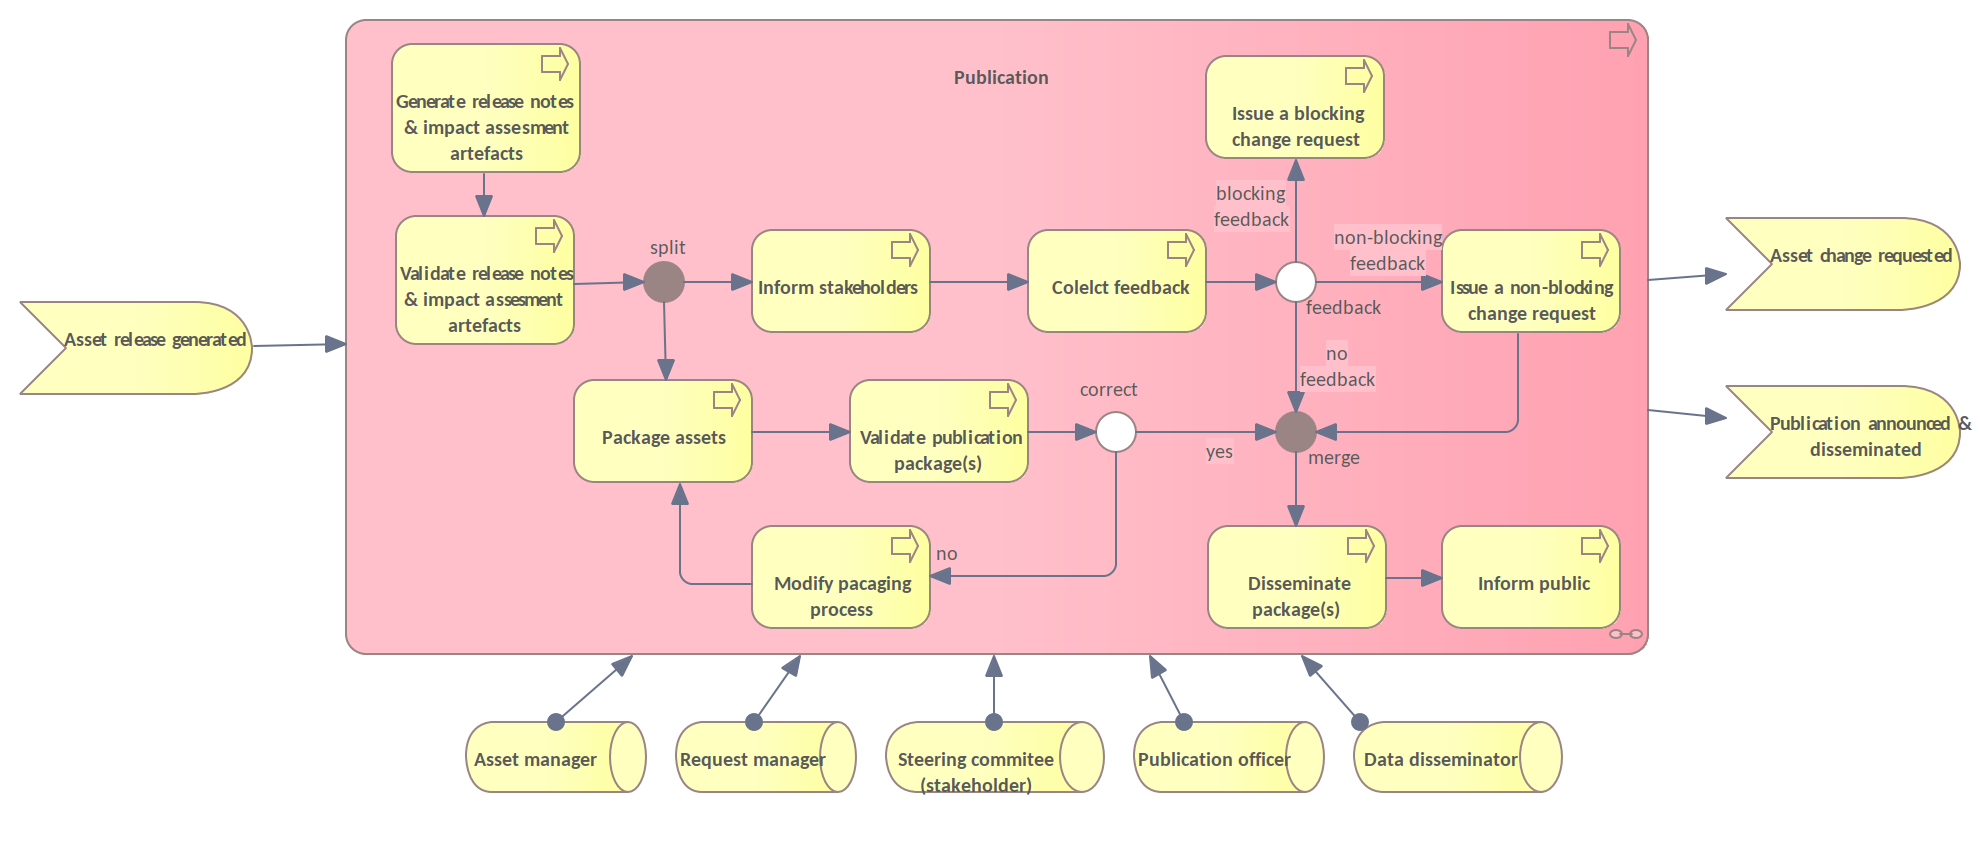
\includegraphics[width=1.05\textwidth]{images/business/new/Publication.png}
		\caption{The new process for the release stage}
		\label{fig:publication-new}
	\end{figure}

	The main difference in this process is the starting point. If currently it starts by transforming and converting the asset source into all forms and formats demanded by the clients, then the new process starts from the premise that the entire publication content has already been generated. 
	
	The new process stats by generation of the release notes and the sett of impact assessment reports destined for different stakeholders. This communication artefacts are verified by the asset manager and then the request manager spreads the news to the stakeholders and the broad public about the upcoming publication. The stakeholders may have a veto or comment on the current publication, just like it currently foreseen.   
	
	What is left, at this stage, from the technical point of view, is packaging and distributing of the publication packages to the data disseminators. The process ends when the latest version of published assets are accessible via the selected data disseminators and the broad public is informed about this. 
	
	This section finishes the description of the business architecture. Next is presented the the application architecture accounting for necessary services and capabilities that must be in place in order to serve the current business processes along with an account of what components realize such services. 
	
\chapter{Application architecture}
\label{sec:application-architecture}

    This section covers the application architecture (term from ArchiMate language). We present here the essential services and the components realising those services to enact the current and the new life-cycle processes.

	\section{Prototypical application structure}
	
	This section presents the application architecture from the solution architecture point of view. A generic solution architecture is depicted in Figure \ref{fig:application-view}.
	
	The application architecture presented covers the application as a ``white box'', its internal component structure, services and interfaces with adjacent applications. Typically the solutions architecture takes the technology aspects into account, accounting for parts of the infrastructure.
	
    \begin{figure}[h]
		\centering
		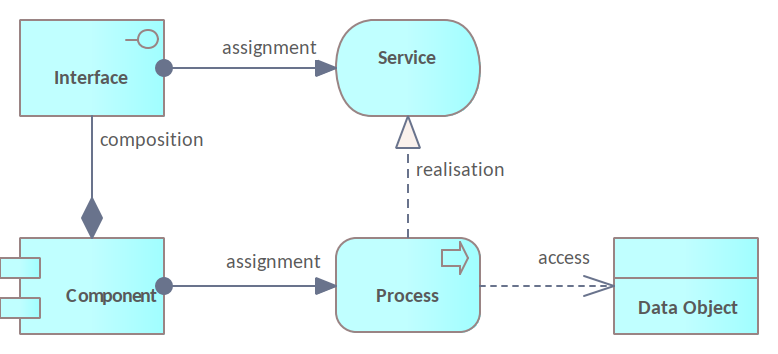
\includegraphics[width=.6\textwidth]{images/views/Application view.png}
		\caption{The prototypical application structure view}
		\label{fig:application-view}
	\end{figure}

	The central element of the application architecture is the \textit{application service}, which represents application behaviour or functionality. The application services, from an inter-layer perspective, serve the processes in the business layer and provide support for their realisation. 
	
	The application services are realised through application processes. The processes have application components assigned to them signifying their place of encapsulation. Application components are modular and replaceable blocks encapsulating implementation of application services and functionalities. In practice, for clarity, we take a shortcut, and say that the application services are realised through \textit{application components} directly.
	
	Components are said to expose interaction \textit{interfaces} which are modelled, in ArchiMate, as proper parts of the components. The interfaces are assigned to services signifying how the latter are to be accessed and consumed. 
	
	Also, components, as well as processes they encapsulate, access \textit{data objects}, which are passive components of the application architecture.

	The solution architecture presented in this section is an adaptation of the generic architecture. Here we focus on presenting what application services are used to support each business process. Moreover, we are interested in grasping the difference in the application layer, between the current and new versions of the business processes. 
	
	To do so, we split the application view diagrams into three vertical lanes. The left lane hosts the current version of the business process as well as the application services and components that are used to support it. In the right lane, we place the new business process and the new application services and components that will have to be adopted for the digital transformation. The middle lane hosts the services and components that are are currently employed and will be carried over into the new application architecture: they are common to both the current and new architectures.

	Below we present an overview of the application architecture, in terms of services alone, depicting how the asset life-cycle stages are served.
	
	\section{Current and new application service architecture}
	\label{sec:application-overview}
	
	This section presents how the asset life-cycle stages are supported by the application services. The current application architecture is depicted in Figure \ref{fig:application-current} and the new one in Figure \ref{fig:application-new}. The services employed in each of the architectures are mostly the same, with a few exceptions. What differs more significantly is their utilisation in the asset life-cycle stages. For this reason, we set them side-by-side to provide a contrasting image. 
	
	\begin{figure}
		\centering
		\begin{minipage}{0.485\textwidth}
			\centering
			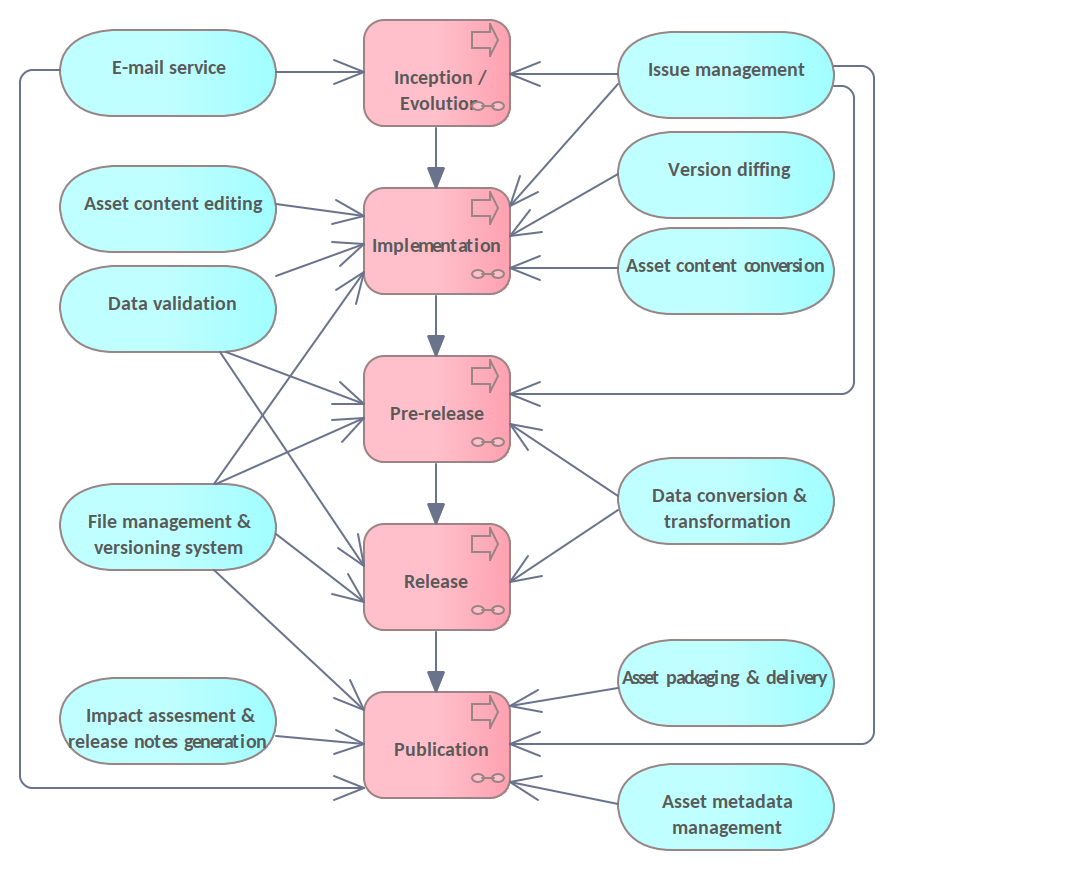
\includegraphics[width=1.3\textwidth]{images/application/Application Services (current).png}
			\caption{The application services that serve the current asset lifecycle}
			\label{fig:application-current}
		\end{minipage}\hfill
		\begin{minipage}{0.485\textwidth}
			\centering
			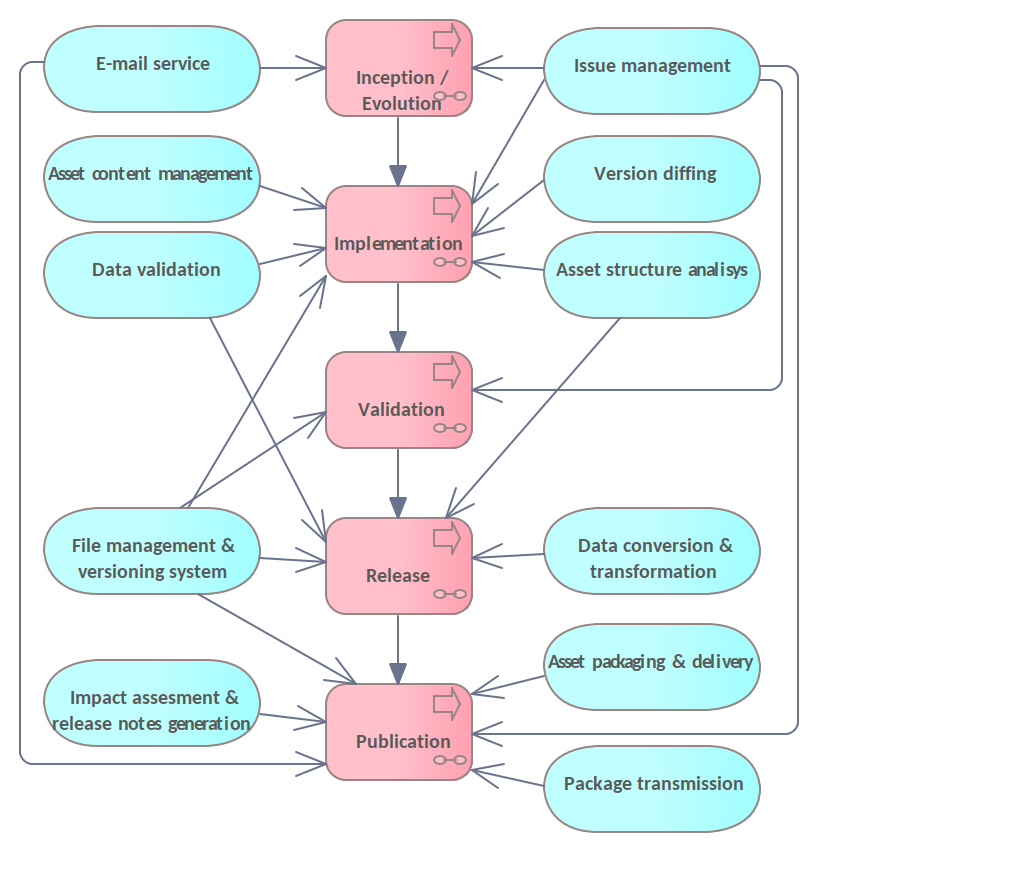
\includegraphics[width=1.3\textwidth]{images/application/Application Services (new).png}
			\caption{The application services that serve the new asset lifecycle}
			\label{fig:application-new}
		\end{minipage}
	\end{figure}
	
%	\begin{figure}[h]
%		\centering
%		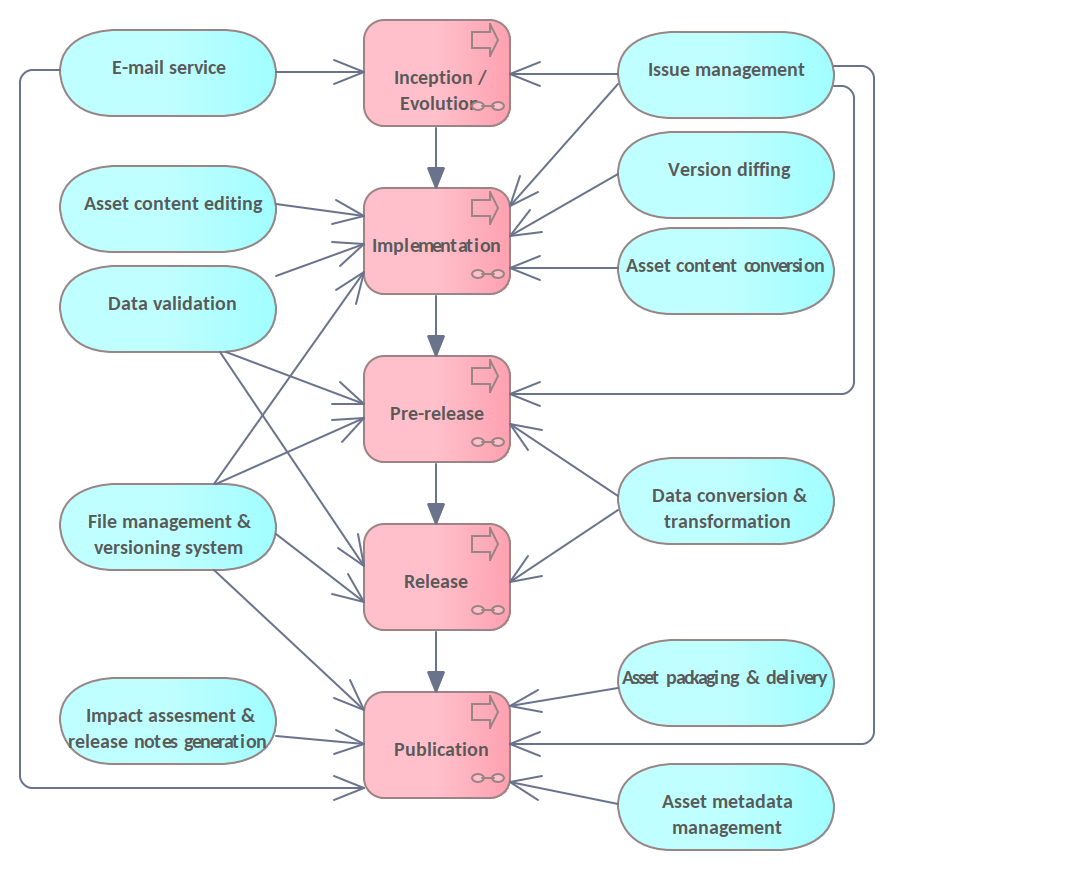
\includegraphics[width=.75\textwidth]{images/application/Application Services (current).png}
%		\caption{The application services that serve the current asset lifecycle}
%		\label{fig:application-current}
%	\end{figure}

	We start the description from the top of the diagram following the sequence of process stages. First is the \textit{e-mail service}. It represents the entire set of capabilities for sending emails covering both the email server and email client. This is realised via the Outlook system \citep{outlook}. 
	
	The \textit{issue management} service represents the capability of recording, documenting and analysing a change request case in a distributed collaborative manner between multiple roles and actors. This is realised via the Jira system \citep{jira}. 
	
	\textit{Asset content editing} is the service which enables the documentalists in the team to modify asset content and hence implement the request cases. This service is realised by MS Excel desktop software \citep{excel}.
	
	The \textit{asset content conversion} service implements the conversion between MS Excel workbook and CAT-XML forms of the asset content. The two representations are equally expressive and the conversion process runs in both directions $ Excel \rightarrow XML $ and $XML \rightarrow Excel $.
	
	\textit{Version diffing} is a service which calculates and presents the difference between two versions of the same asset. The \textit{data validation} service is self-explanatory. It checks whether the asset content is correct, or not. The asset content conversion, version diffing and data validation services are realised by components that comprise the legacy workflow, which is currently in use.
	
	\textit{Asset document management} provides capabilities for describing, storing and producing documents about assets in various human-readable formats (e.g. HTML, PDF, docx). It also allows for document metadata management. Currently, this capability is realised by PDF forms, called Asses Document Description (ADD), which are produced from XML-DITA sources \citep{dita-day2005introduction, dita-spec} using Adobe FrameMaker \citep{framemaker} . 
	
	\textit{Asset metadata \& workflow management} is a service which centralises the flow of the automated processes. It is currently realised by legacy workflow implementation. 
	
	The \textit{file management \& versioning} service enables storing the content and and tracing the evolution of assets. This service is realised by the SVN system \cite{svn}.
	
	The \textit{data transformation} service is self-explanatory. It stands for a generic capability of transforming data from one form and format into another. Currently, this service is realised by a multitude of custom-built transformation procedures, some of which are chained to produce the desired outcome. This service is realised by components that are part of the legacy system. 
	
	The \textit{asset packaging} service prepares assets for transmission to the partner distribution systems, specifically Cellar. It covers functionalities including assembling the necessary asset representations together with their documentation, generating necessary technical metadata and zipping the assets in a manner that is acceptable for partner distribution systems. The type of package and the asset metadata description varies, yet among the most prominent ones are METS \citep{mets}, IMMC\footnote{see \url{https://op.europa.eu/en/web/eu-vocabularies/immc}} and DCAT \cite{dcat2}. 
	
	The last service to mention that is employed in the current life-cycle process is the \textit{impact assessment \& release note generation} service. Its title is again self-explanatory. The values it provides are the release notes that are published with assets and describe the list of changes implemented in each version. The impact assessment is a type of report which includes assessments for target stakeholders which usually are service provides whose systems depend on the assets published by the SU. These special impact assessments may target whether a given aspect of an asset has changed which may disrupt functioning systems. So, a series of specific checkers and reports are produced to safeguard the partners. 
	
	The new application architecture (Figure \ref{fig:application-new}), as mentioned above, re-configures how services are used across process stages. It replaces the asset content editing service by a new one which is \textit{asset content management}. This service is realised by a fully-fledged semantic web editing system -- VocBench3 \citep{stellatovocbench}. In addition, two more services are added: asset structure analysis and package transmission services.
	
	The \textit{asset structure analysis} implements an automatic fingerprinting of the asset structure which provides an insight into how the managed asset is realised and substantiated. This fingerprinting serves as an indicator for the structural validation in the implementation step. For example, a missing or extra property will be spotted with this service. 
	
	The \textit{package transmission} provides the possibility to automatically deliver and ingest the prepared packages into the dissemination system, rather than the publication officer having to perform this operation manually. 
	
%	\section{New application service architecture}
%	\label{sec:application-new}	

%	\begin{figure}[h]
%		\centering
%		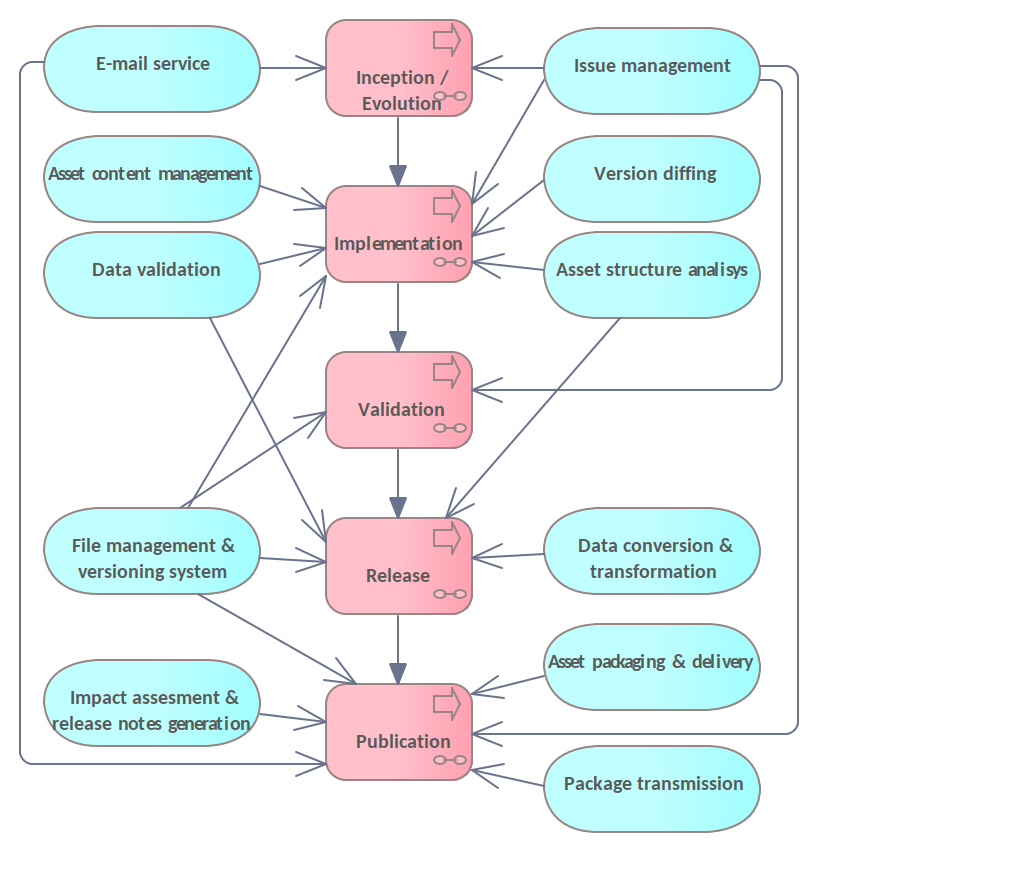
\includegraphics[width=.75\textwidth]{images/application/Application Services (new).png}
%		\caption{The application services that serve the new asset lifecycle}
%		\label{fig:application-new}
%	\end{figure}	
	
	\section{Inception and evolution services and components}
	\label{sec:evolution-application}
	
	In the first stage of the asset life-cycle, the technical requirements are limited to client communication and the request documentation services as depicted in Figure \ref{fig:application-inception-evolution}.
	
	\begin{figure}[h]
		\centering
		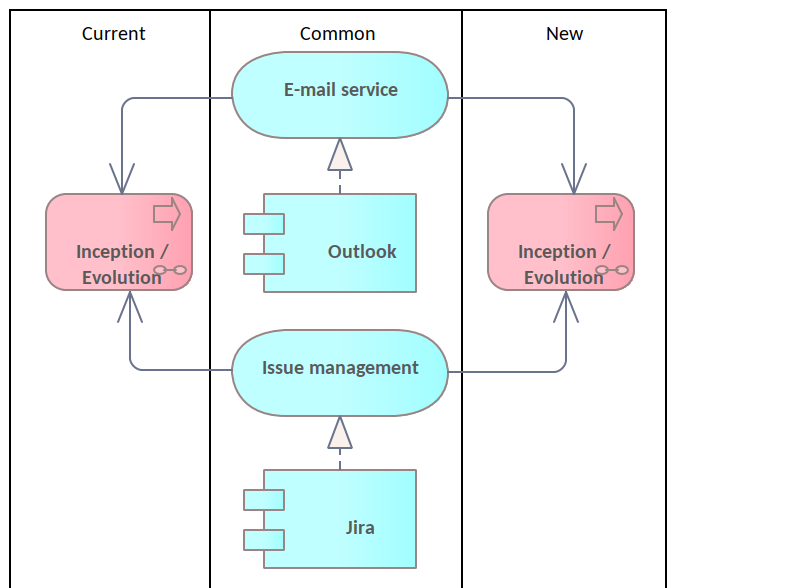
\includegraphics[width=.6\textwidth]{images/application/InceptionEvolution.png}
		\caption{The application services and components that serve the current and new inception and evolution stage}
		\label{fig:application-inception-evolution}
	\end{figure}
	
	In the left and right lanes of the diagram are where the current and new life-cycle stages are represented as red rectangles. In the middle lane are the email and issue management services because they are involved in both the new and current architectures. 
	
	The email service is realised by the Outlook software. Issue management is realised by the Jira system. No changes are foreseen in the way these services are realised in the future. 

	\section{Implementation services and components}
	\label{sec:implementation-application}	
	
	The implementation stage is the first place where considerable differences are visible in the way the application architecture is organised. This is depicted in Figure \ref{fig:application-implementation}.
	
	\begin{figure}[!h]
		\centering
		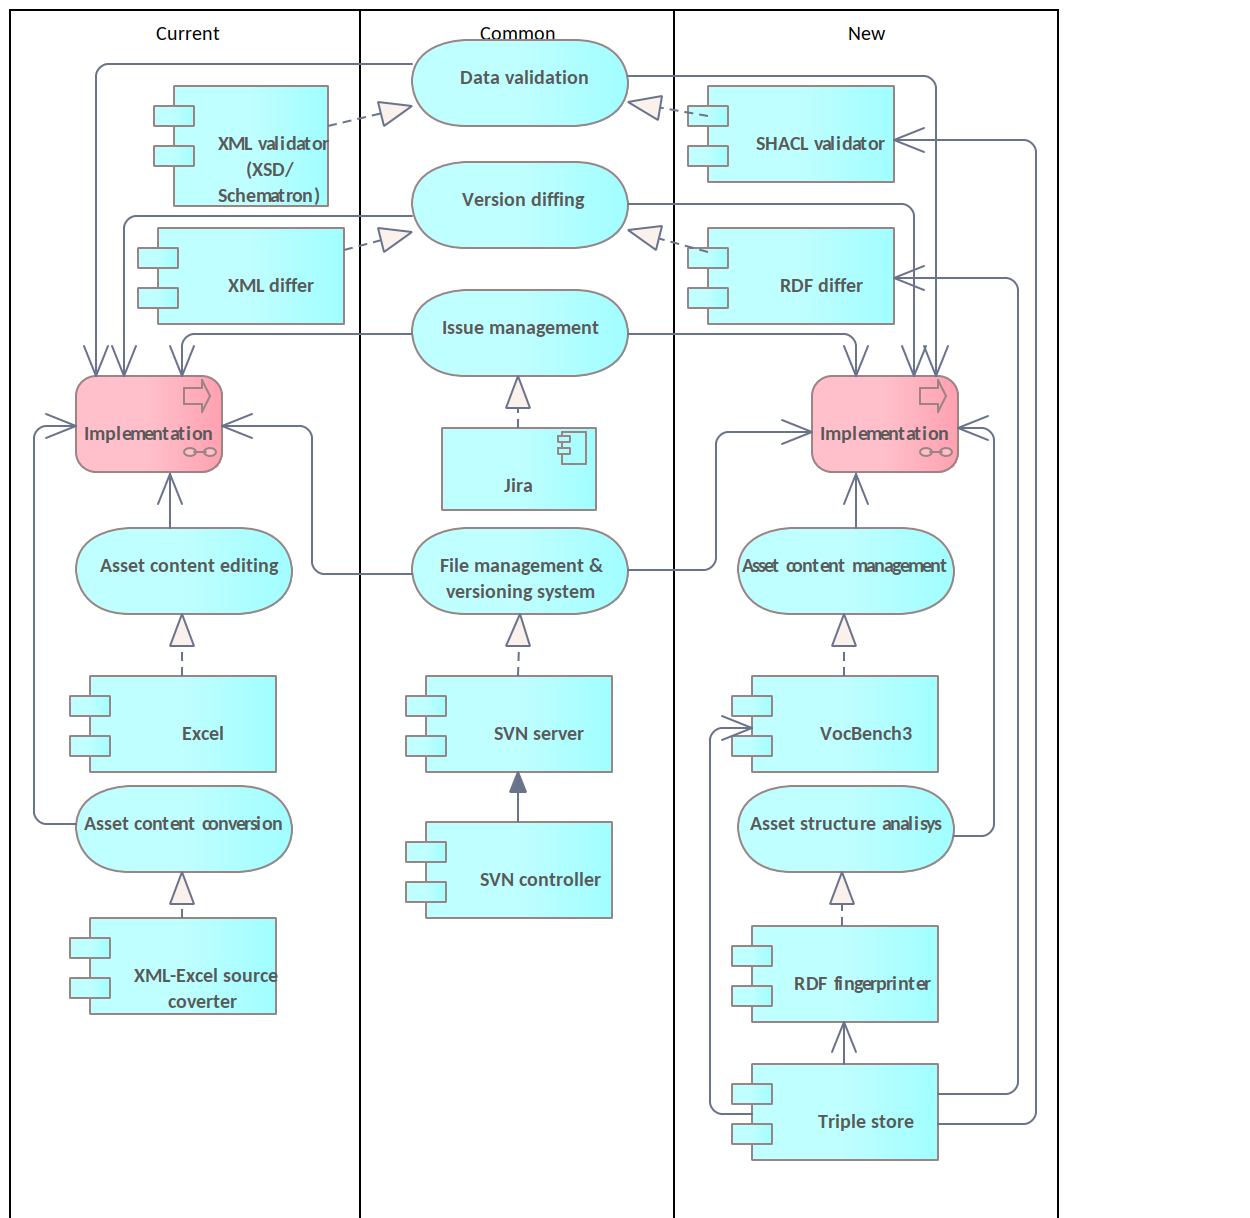
\includegraphics[width=.9\textwidth]{images/application/Implementation v3.png}
		\caption{The application services and components that serve the current and new implementation stage}
		\label{fig:application-implementation}
	\end{figure}
	
	We start discussing this architecture by covering the common services first, situated in the middle lane of the diagram, and then we address particularities which are situated at the left and right sides of the diagram. 
	
	The issue management system is involved and is realised the same way as in the inception/evolution stage (Section \ref{sec:evolution-application}). In the following sections the services and their realisation that have been already discussed will no longer be addressed.  
	
	File management \& versioning is realised through SVN \cite{svn}. In the current application architecture this serves as a foundation for process automation, the triggers being any operations within the SVN repository. The mechanisms employed are similar to what an automation server is doing in the software development context: triggering automatic building, testing and deploying, facilitating continuous integration and continuous delivery. No such automation server is, however, used due to infrastructure limitations that existed in the past and a custom SVN handler component was developed within the legacy workflow system. 
	
	In the new architecture, the possibility to continue the same practice of automating process executions based on SVN triggers is still there. Moreover, we recommend replacing the current SVN handler by an automation system, such as Jenkins \citep{jenkins} and Bamboo \cite{bamboo}. This suggestion is not depicted in the diagram because the current workflow SVN handler could still serve in the immediate future; however, for the long run, we recommend an alternative.
	
	Asset metadata and workflow design management is centralised in a custom-built XML file called the "Vocabulary table". The vocabulary table is a file which contains descriptions of currently-administered digital assets, descriptions of generic process execution flows and decision rules for special assets. For this reason, we say the it is "workflow design management" and not the actual "workflow management",  because we deal here with description and configuration of the execution paths and decision rules (plus asset metadata) which are enacted by the legacy workflow system. This aggregation of the two responsibilities complicates both the maintenance and evolution both shall be separated in the future.  
	
	Later, after adoption of the digital transformation proposed in this architecture, the asset metadata and workflow design management service need to be broken down into two parts: asset metadata management and workflow management. The metadata management can be realised through a DCAT \citep{dcat2} cataloguing software. 
	
	Workflow management could be taken over by any workflow management and execution engine that implements service orchestration\footnote{In system administration, orchestration is the automated configuration, coordination, and management of computer systems and software. A number of tools exist for automation of server configuration and management, including Ansible, Puppet, Salt, Terraform, and AWS CloudFormation.} or choreography\footnote{Service choreography is a form of service composition in which the interaction protocol between several partner services is defined from a global perspective.}. 
	
	This could be taken one step further towards a BPMN \citep{bpmn-introduction} execution engine such as Camunda BPM, Flowable and Bonita BPM. There is an installation and configuration overhead for such a system, but the investment is worth considering knowing that they ship with tools for creating workflow and decision models, operating deployed models in production, and allowing users to execute workflow tasks assigned to them. 
	
	Now we should focus on the top of the middle lane, to the data validation and version diffing services. The components that realise them are split between the left and right lanes. This means that currently validation is performed using the XML validator and the version diffing is performed using XML differ, while in the new application, validation is realised using a SHACL \citep{shacl-spec} validator, and version diffing using an RDF differ. The SHACL validator and RDF differ are custom components developed for the new application context.
	
	In the right lane, the asset content editing and the asset content conversion services were introduced in Section \ref{sec:application-overview}. They are the gateway for the asset authoring officers to implement change request cases. Content editing is realised through MS Excel running on the documentalists' workstations. Once the edit is finished, the updates are committed to the common SVN repository. The changes are picked up by the SVN handler in the legacy workflow system and trigger a conversion process from MS Excel to XML, and then back to MS Excel. The conversion is realised by another legacy component implemented to do exactly that. The resulted conversion is committed into the SVN repository again. This circular conversion, as explained in Section \ref{sec:implementation-current}, is necessary because the main source of the assets is represented as CAT-XML, whereas MS Excel workbook is merely an extension that enables user-friendly editing capabilities.
	
	In the new version of the implementation stage, the main source of the assets is represented as SRC-AP \cite{src-ap-vb3}, a particular form of SKOS \citep{skos-spec} and is serialised as RDF \citep{rdf11}. The editing is covered by the asset content management service, which is realised by the VocBench3 system \citep{stellatovocbench}. When the authoring officer finishes the implementation of a request case, the content is exported from VocBench3 and committed into the SVN common repository. This commit triggers automatic SHACL validation, RDF diffing and structure analysis operations, which write the results back into the common repository for the editor to look at and verify the implementation correctness. 
	
	Asset structure analysis service is realised by the RDF fingerprinter component which is necessary for the quality assessment in this and the next stage of the asset life-cycle. Finally, asset documentation management service was described in \mbox{Section \ref{sec:application-overview}.}
	
	The new RDF-based components rely mostly on the existence of an RDF triple store service, which is a database ensuring persistence, accessibility and data query. This triple store component is depicted not as realising any service in particular, but as serving other components: RDF fingerprinter, SHACL validator, RDF differ and VocBench3, so that they function as expected this way, creating a dependency between them. We use a generic label ``triple store'' here to express that it is of little importance what system is chosen in particular. Among the candidates we can mention are Fuseki, Virtuoso, GraphDB, StarDog, AnzoGraph,... the list can continue. 
	
	This brings us to the end of the implementation stage description which provided us with a parallel between the services and components as they are used currently and how the new application should be implemented. 
	
	\section{Pre-release and validation services and components}
	\label{sec:validation-application}
	
	The stages following the implementation in both the current and new life-cycle processes differ. In Section \ref{sec:lifecycle-new} we described that in the current life-cycle it is termed the pre-release stage while in the new one it is the validation stage. This difference is also reflected on the application architecture in Figure \ref{fig:application-validation}.
	
	\begin{figure}[h]
		\centering
		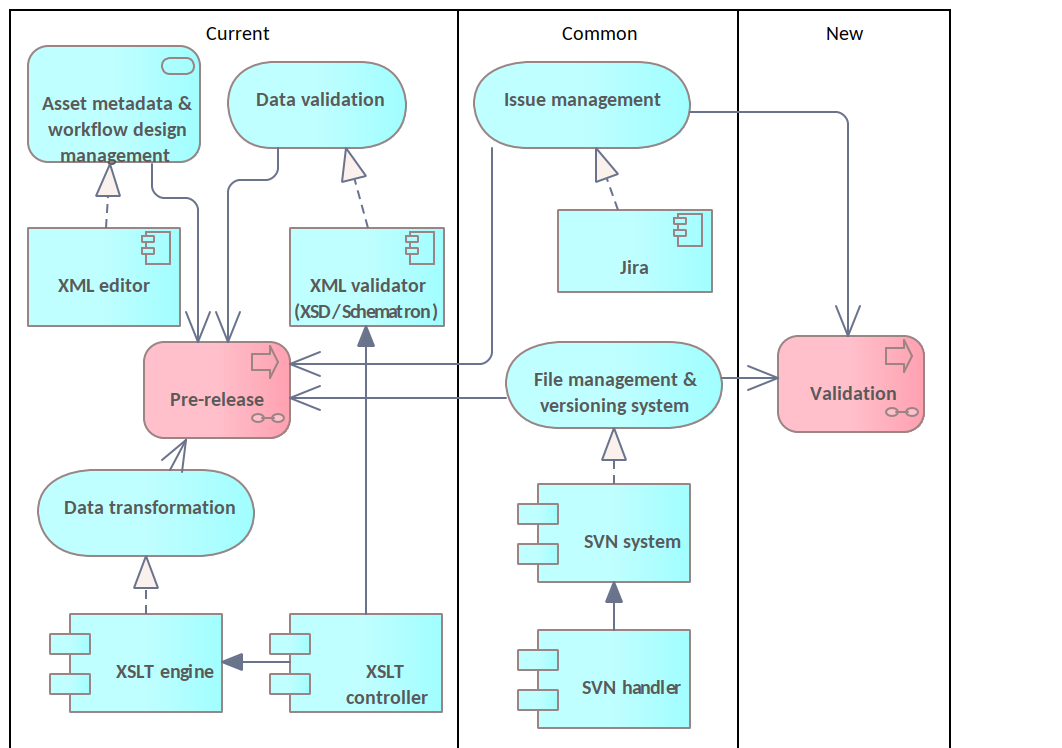
\includegraphics[width=.9\textwidth]{images/application/Validation & Pre-release v3.png}
		\caption{The application services and components that serve the current pre-release and the new validation stages}
		\label{fig:application-validation}
	\end{figure}
	
	The current pre-release stage, on the left lane of the diagram, involves asset metadata and workflow design management service, described in Section \ref{sec:implementation-application}, due to the workflow automation involved in this stage. 
	
	The data validation was also described in Section \ref{sec:implementation-application}. One thing that was not mentioned is that the validation relies on an XSLT \citep{xslt3-Kay} controller component which triggers the XML validator component, also the XSLT transformation component realising the data transformation service.
	
	The data transformation service is used currently in the pre-release stage to format the RDF/XML content. Internally, this operation is known as SKOS ``prettification'', i.e. making the SKOS-RDF/XML easier to work with. This operation will no longer be necessary in the new architecture and the XSLT transformation component will only be employed in the next stage: release.
	
	The issue management, file management and versioning services are used in the pre-release stage and are the only ones necessary in the validation stage. Therefore, they are placed in the middle, common, lane. These services have been detailed in Section \ref{sec:evolution-application} and \ref{sec:implementation-application}. The validation stage requires nothing more than these because it is mostly a manual process executed by the validation officer who checks the validation artefacts generated previously in the implementation stage, as explained in Section \ref{sec:validation-new}.	

	\section{Release services and components}
	\label{sec:release-application}	
	
	The release stage is significantly unbalanced in terms of the services employed currently and what is foreseen in the new architecture: this is reflected in the application architecture depicted in Figure \ref{fig:application-release}. 
	
	\begin{figure}[h]
		\centering
		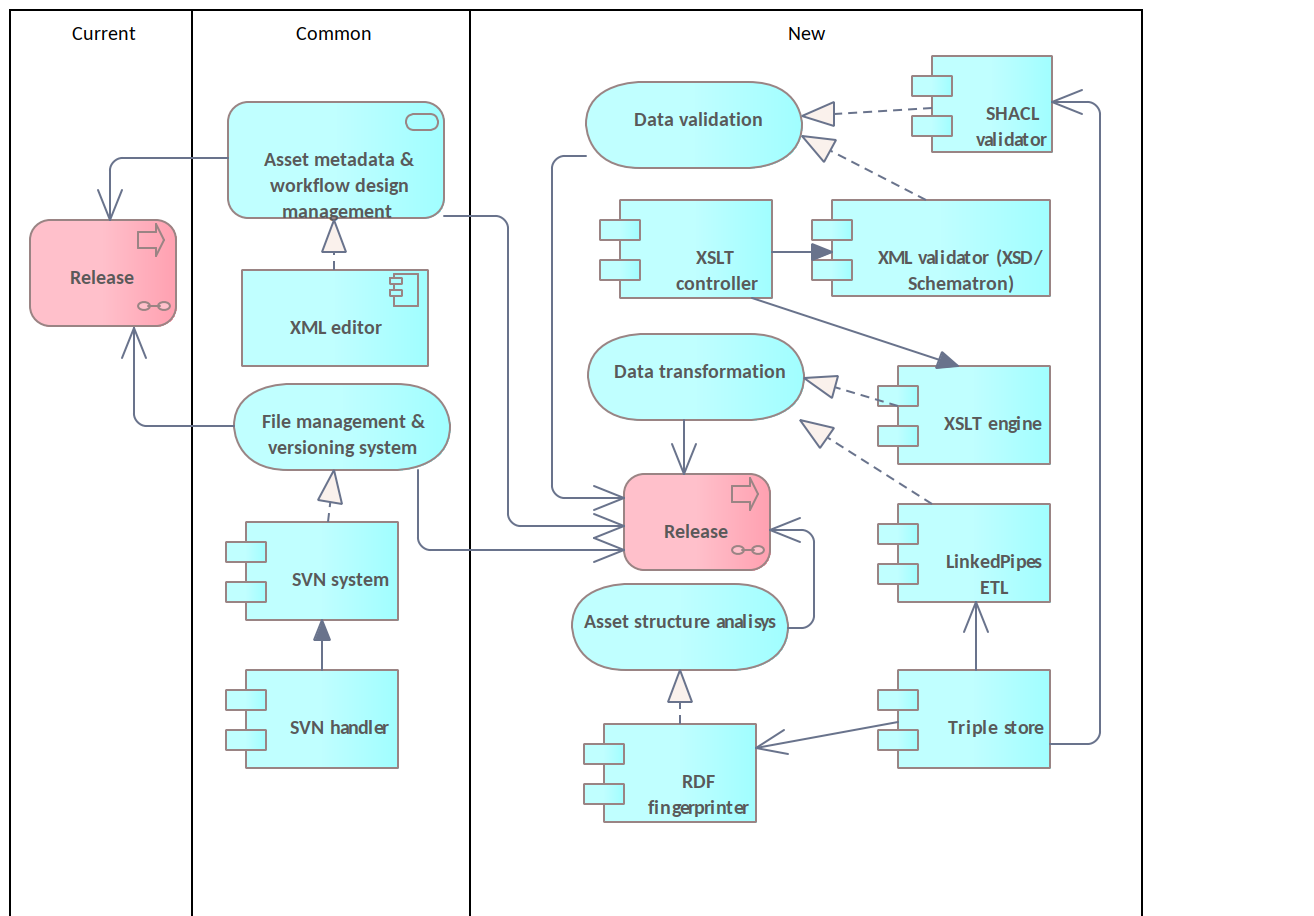
\includegraphics[width=.9\textwidth]{images/application/Release v3.png}
		\caption{The application services and components that serve the current and new release stage}
		\label{fig:application-release}
	\end{figure}

	Currently, in the release stage described in Section \ref{sec:release-current}, the asset(s) are mainly copied from one part of the common repository into a another which is dedicated to the artefacts that follow to be published. 
	
	In the new release stage, in addition to the copying operation, all data transformation operations described in Section \ref{sec:publication-current} are also executed leaving the (new) publication stage to deal with packaging and distribution mainly (from a technical perspective).
	
	This is reflected in the new application architecture depicted in the right lane. The data transformation services are employed here, not only in their current form, dealing with various formats consumed by the current clients (XSD, MarkXML, GeoJSON, etc.), but also with complex transformation operations on RDF representation. The former is realised through the same XSLT engine component, while the latter is realised through a new component called LinkedPipes ETL \citep{linkedpipes-klimek2016linkedpipes,linkedpipes-klimek2017linkedpipes}.
	
	The situation is similar with the data validation service: both the current validation component based on XSD schemas and Schematron checks, and a new validation based on SHACL shape checks, are necessary. Both validation types are used because current data formats and new data formats needs to be formally verified before being published. This validation, however, aims to ensure primarily that the transformation processes run correctly and, to a lesser effect, the content correctness which is already assessed in the previous validation stage. The asset structure analysis service was addressed in Section \ref{sec:implementation-new}. Also, the new components that operate with RDF data require a triple store which is depicted in the left lane as serving the depending components.
	
	
	\section{Publication services and components}
	\label{sec:publication-application}	
	
	The publication stage is the last one in the asset life-cycle process. Its application architecture is depicted in Figure \ref{fig:application-publication}. There is not much difference between the two, most services and components being placed in the middle lane, common to both. 
	
	\begin{figure}[!h]
		\centering
		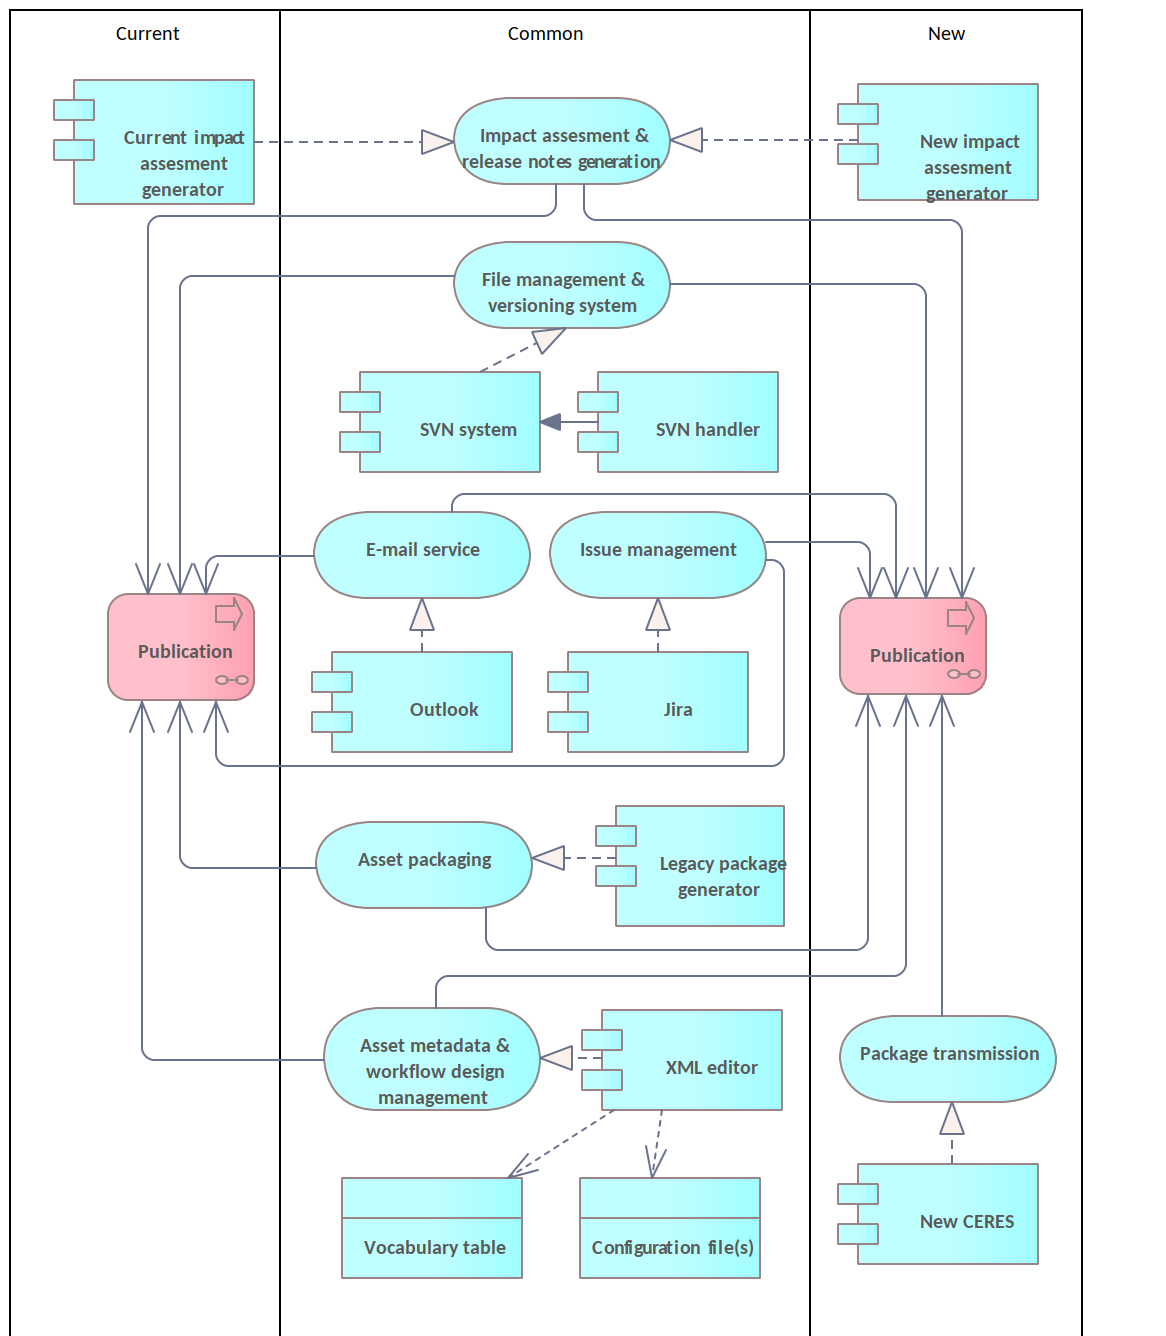
\includegraphics[width=.9\textwidth]{images/application/Publication v3.png}
		\caption{The application services and components that serve the current and new publication stage}
		\label{fig:application-publication}
	\end{figure}

	New and specific to the publication stage is the impact assessment. The release notes generation service provides the basic communication artefacts about what has changed between two versions of an artefact and what is contained in a publication. To a large extent, it is based on the diffs generated in the implementation stage, but not limited to those. However, this has an impact on how the component functions because the diffs of two XML files are different from the diffs of two RDF files. The asset source format changes from XML to RDF in between the current and new architectures: therefore, the current implementation of the service cannot be reused and a new impact assessment generator shall be developed for the new application. 

	The following services have already been addressed in the previous sections and are not discussed here: management and versioning, e-mail, issue management and asset metadata and workflow design management. 
	
	The asset packaging service, placed in the middle lane of the diagram, is another service that is specific to the publication stage only. It is realised by the legacy package generator which assembles in various ways asset artefacts as necessary for partner dissemination systems and final consumers. This component shall be reused in the new application architecture in order to ensure continuity: however, it may be replaced in further digital transformation initiatives. 
	
	The last service adopted in the new application architecture is the package transmission service. The added value of this service is that the publication officer does not any more need to manually ingest the packages into the dissemination system. For a start, this service is realised by the new CERES component which is responsible for ingesting packages into Cellar. Later on, additional components can be created for ingesting packages into other dissemination systems such as Wikidata, Bartoc, ODP, etc. 
	
	This brings us to the end of the application architecture description. Next we will take a look at how the two applications are deployed in practice and the differences in the infrastructure.
\chapter{Technology architecture}
\label{sec:technology-architecture}

    This chapter covers the technology architecture (term from the ArchiMate language). It is used for modelling the underlying infrastructure and deployment of applications as software, servers, clusters, load balancers, etc. The next section presents a generic pattern which we substantiate in this architecture. 
    
	\section{Prototypical technology structure}
	
	This section presents a generic technology architecture organisation, depicted in Figure \ref{fig:technology-view}, in order to ease interpretation of the diagrams that follow.
	
	\begin{figure}[!h]
		\centering
		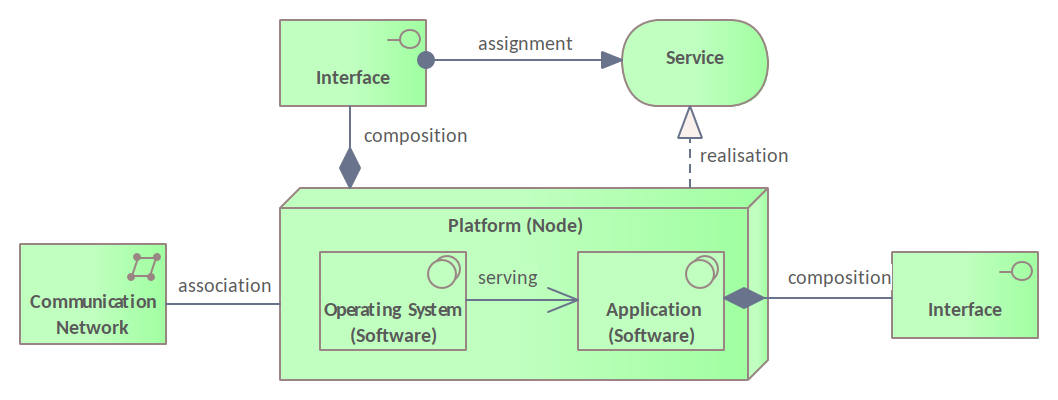
\includegraphics[width=.75\textwidth]{images/views/Technology View.png}
		\caption{The prototypical technology view}
		\label{fig:technology-view}
	\end{figure}

	The central concept in the technology view is the node. It represents a computational or physical resource that hosts, manipulates or interacts with other computational or physical resources. Within a node, various software components are deployed, most foundational of which is the operation system. The node aggregates various software. 
	
	Depending on the chosen level of granularity, nodes may realise technology services which represent explicitly defined and exposed behaviour. Also, nodes and software may expose interfaces which represent points of access where a technology service offered by a node can be accessed. Interfaces constitute parts of the node: an interface may be assigned to a service.
	
	Lastly, node are connected to the communication network which represents a set of structures that connects nodes for transmission, routing and reception of data. There may be one or more networks depending on the organisation security policies and on the internal infrastructure setup. These ArchiMate elements suffice to describe the current and new technology architectures. 	
	
	\section{Current technology architecture}
	\label{sec:technology-current}
	
	The current SU infrastructure necessary to support the application life-cycle is depicted in Figure \ref{fig:technology-current}. It comprises four nodes for a private network and a controlled connection to the internet. 
	
	\begin{figure}[!h]
		\centering
		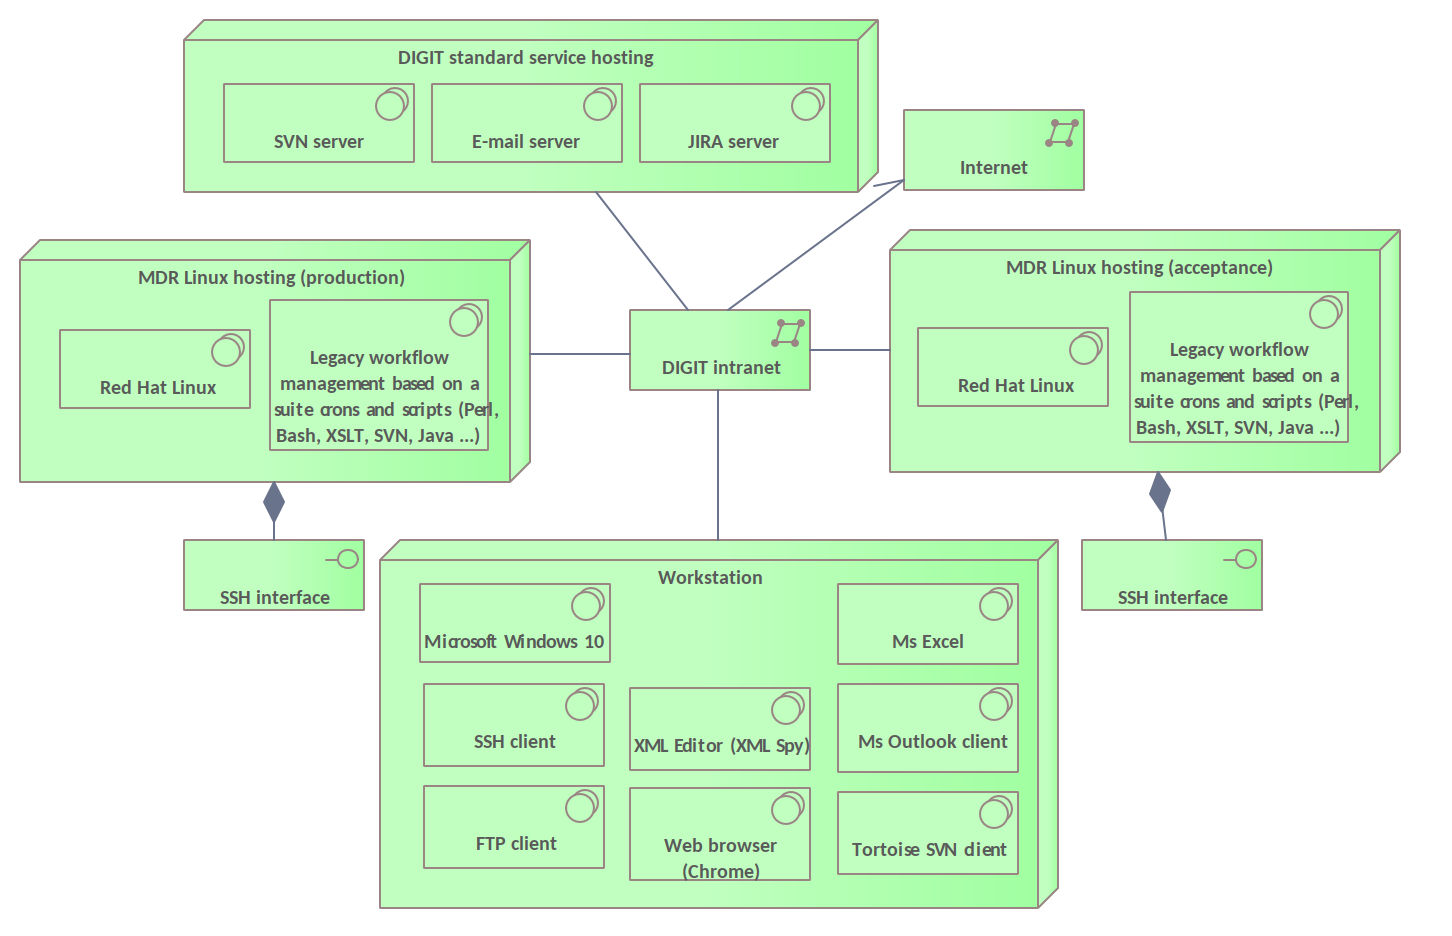
\includegraphics[width=1.01\textwidth]{images/technology/Current Platform.png}
		\caption{The technology structure that supports the current asset lifecycle}
		\label{fig:technology-current}
	\end{figure}
	
	At the bottom of the diagram is the workstation node which represents the standard machine provided to the members of the SU team by the DIGIT infrastructure unit. The workstation runs Windows 10 \citep{windows10} operating system and the following set of tools (at least) are installed on it: MS Excel, Outlook, Chrome (os another modern browser), an SVN client (Tortoise SVN is the default choice by the SU team), a specialised XML editor (XML Spy is the default), an FTP client of choice and an SSH client (Putty is the default). This set of software is used to perform all the necessary duties and enact the described business processes. 
	
	At the top of the diagram is depicted the standard service hosting offered by DIGIT. The provided services there are the e-mail service, a dedicated the SVN repository as a service and a set of Jira projects.
	
	In addition, two identically-housed Linux servers are provided: one acting as the acceptance environment and the second as the production environment. They are registered at DIGIT as ``MDR Linux hosting'' nodes and they host the legacy workflow management system. This legacy system is based on multiple technologies which were added gradually and organically in the course of its development. It includes components written as Perl scripts, Bash scripts, many XSLT transformation style-sheets, commends relying on existence of an SVN client and Java libraries and scripts.
		
	One of the MDR Linux hosting nodes serves for testing purposes and the other one an operational environment for production. The nodes run RedHat Linux 7.7 operating system and each expose an SSH interface. These interfaces are used by the technical team. The technical team member connect using SSH from their workstations and operate the legacy workflow management system remotely.
	
	The communication network is secured as an intranet-authenticated connection provided by DIGIT. From the intranet, a controlled access to the Internet is available through an authentication proxy. 
	
	This completes the description of the current infrastructure architecture and sets the baseline for the new architecture described in the next section.
	
	\section{New technology architecture}
	\label{sec:technology-new}
	
	The new infrastructure architecture is depicted in Figure \ref{fig:technology-new}. What are the same as in the current one are the structure of the workstation node, the intranet and the Internet connections, as well as standard hosted services to which are added VocBench3 and the Adobe FrameMaker server which are necessary for realising the asset description documentation (ADD) service, in addition to a few other important services within SU, among which is the generation of the Interinstitutional Style Guide. 
	
	\begin{figure}[!h]
		\centering
		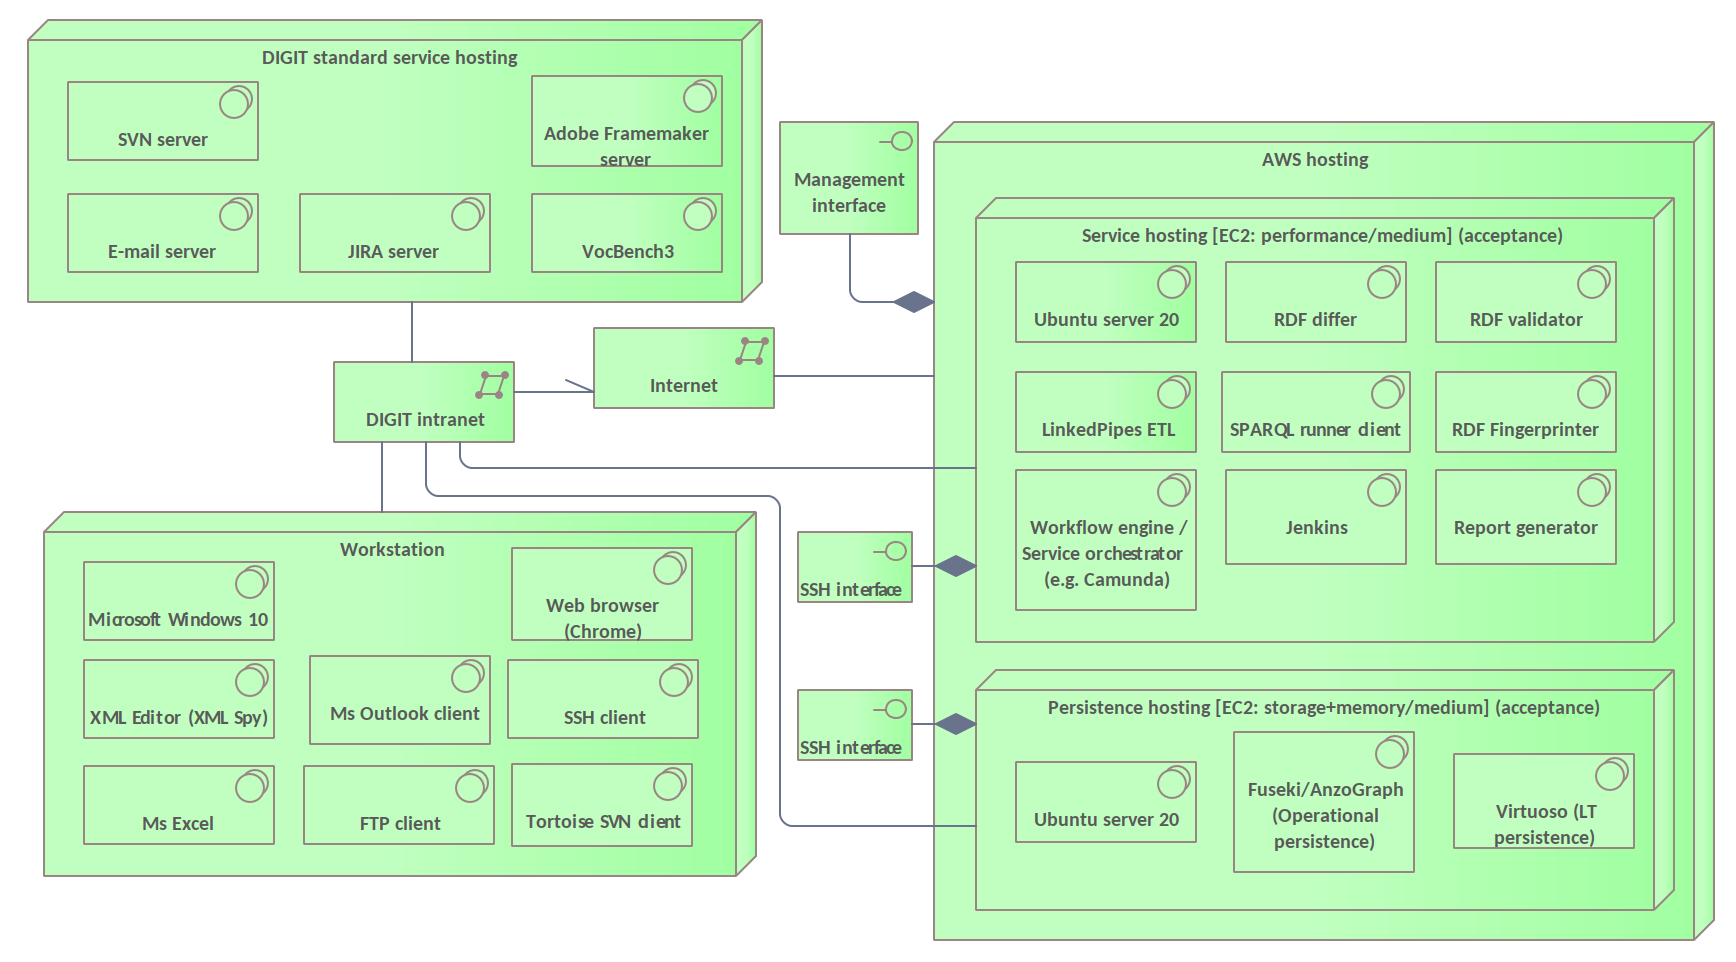
\includegraphics[width=1.01\textwidth]{images/technology/New Platform.png}
		\caption{The technology structure that supports the new asset lifecycle}
		\label{fig:technology-new}
	\end{figure}

	What differs significantly between the two is the disappearance of the hosted nodes (left and right side of Figure \ref{fig:technology-current}) and their replacement with dedicated Amazon Web Service (AWS) hosting, depicted as a large node on the right side of Figure \ref{fig:technology-new}. This node exposes a management interface which provides the possibility of configuring and launching multiple virtual servers (called EC2 instances) of various sizes and performance capabilities. This puts an administration overhead onto the SU team, but also frees it from a large number of constraints and experiences in the past years, this way smoothing the path for this and future digital transformations.
	
	In the new architecture, to support the application architecture described in Section \ref{sec:application-architecture}, two instances are necessary: one optimised for performance and another optimised for persistence. The first one hosts the operational application components, while the second one hosts the triple stores and potentially other types of databases. This initial separation into two could be further optimised by moving some services to dedicated EC2 instances if deemed necessary. Also, these two instances are considered an acceptance environment where the new application is assembled and tested. Once it is ready to move into production, an identical copy of EC2 instances is created and those are further used for production operations. 
	
	The EC2 instance at the top, marked for performance, runs a Linux OS, preferably Ubuntu 20 or RedHat 8, and has installed the following software: RDF differ (custom-built component), RDF validator (custom-built component), RDF fingerprinter (custom-built component), LinkedPipes ETL, Jenkins automation system and optionally Camunda BPM. 
	
	The EC2 instance at the bottom, marked for persistence, needs to run Ubuntu or RedHat as well, and hosts triple stores: Fuseki (for the custom built components) and for LinkedPipes ETL, which are optimised for operational performance, and an instance of Virtuoso triple store which is meant for long-term preservation of RDF data. 
	Optionally, in the acceptance phase, the triple stores could be hosted on a single EC2 instance to avoid management overheads. 
	
	Each of the EC2 instances expose an SSH interface which can be accessed by the technical team to configure, manipulate and operate the servers, just like in the currently-hosted MDR Linux server. 
	
\chapter{Technology deployment proposal}


	This chapter describes the detailed infrastructure organisation necessary for supporting the new application architecture of the asset publishing life-cycle. This represents the initial setup for starting the transition towards the new architecture and it is likely to evolve. 
	
	We split our presentation into chunks easy to describe, yet it is important to bear in mind that they are not separated parts but views of a larger whole. Some of these views bear names similar to the life-cycle stages but there is no one-to-one correspondence those stages. Rather the view names are formulated based on the presented components.
	
	The deployment proposal in this chapter is mainly focused on the organisation within the AWS nodes depicted in Figure \ref{fig:technology-new}. It nevertheless can occasionally mention other parts of the technology structure such as for example in Section \ref{sec:technology-view-vb3-export}. 
	
	In the current proposal we adopt a service oriented approach as motivated in \ref{sec:soa}. We assume the reader has a basic understanding in how Docker platform \citep{docker} functions and this is linked to the fact that each software element in the diagrams below represents a service deployed and executed as a Docker container. The artefact elements marked with ``data volume'' label represent attached Docker volumes.  
	
% 	\vfill

	\section{VocBench3 export and automation services}
	\label{sec:technology-view-vb3-export}
	
	The aim of this section is to explain what components need to be deployed in order to automate the export of data from VocBench3 and trigger automated processes necessary in the implementation stage of the life-cycle (see \ref{sec:implementation-new}).	
	
	
% 	We explain how to deploy software components so that the export from VocBench3 can be triggered by a software component through an API call or a SU team member through the user interface. Even more so, this export shall automatically trigger other components, which are responsible of diffing, validation and fingerprinting the exported content. 
	
	VocBench3 (the blue block in Figure \ref{fig:technology-view-implementation}) is an application component hosted under the standard DIGIT service agreement, i.e. outside the scope of current infrastructure description. Therefore the assumption is that this software is accessible through its interfaces and no direct configuration is possible. VocBench3 exposes two interfaces: first is an user interface implemented with Angular framework, and second is the API of the Semantic Turkey middleware (ST). The latter can be remotely called by our services, such as for example a ``Semantic Turkey exporter'' which exports the necessary data assets VocBench3 and stores them into a common repository. 
	
	\begin{figure}[!h]
		\centering
		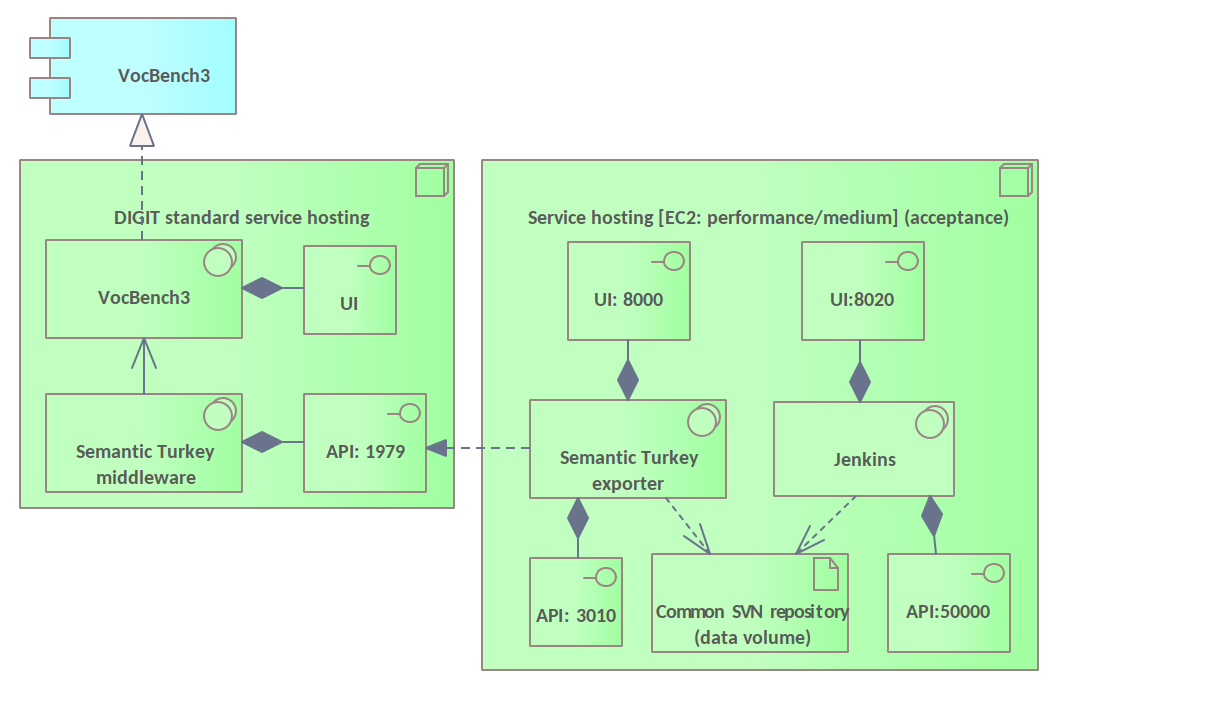
\includegraphics[width=\textwidth]{images/infra-setup/implementation.png}
		\caption{The technology components for exporting asset sources from VocBench3 into the common SVN repository}
		\label{fig:technology-view-implementation}
	\end{figure}
	
	Semantic Turkey exporter component shall be configured according to the Semantic Turkey installation offered by DIGIT (port, address and access rights). This component exposes a user interface and an API which allow exporting a selected project from VocBench3 and committing it into the common SVN component. If such component is missing, this operation can be performed manually until later implementation is available in place. 
	
	An instance of Jenkins automation server should be deployed and configured to listen to changes in the common SVN repository on preselected projects. It can be configured through the user interface or configuration files at the runtime. It also must be configured to trigger execution of RDF differ, RDF validator and RDF fingerprinter on the exported asset(s) and other configurations as necessary. Once an export is committed into the SVN repository Jenkins will automatically trigger chain execution of the pre-configured services. 
	
	The deployment organisation of the validation, diffing and fingerprinting services is described in the next section. 
	
	%This functionality of listening for changes in the SVN repository and firing other services is currently implemented in the legacy workflow component. 
	
	\section{Validation services}
	\label{sec:technology-view-validation}
	
	In this section we explain how SHACL validation, RDF fingerprinting and RDF differ components are deployed illustrated in Figure \ref{fig:technology-view-validation}. Each of the tree components is realised by a software component with a generic name of the function it realises: RDF validator, RDF differ and RDF fingerprinter. Each of these software components exposes two interfaces: one is the user interface and another is an API. The API represents the potential for being operated by an automation server such as Jenkins or an service orchestrator like Camunda. We omit to picture the hosting EC2 node as all the mentioned elements belong to it making it redundant in the diagram.
	
	\begin{figure}[!h]
		\centering
		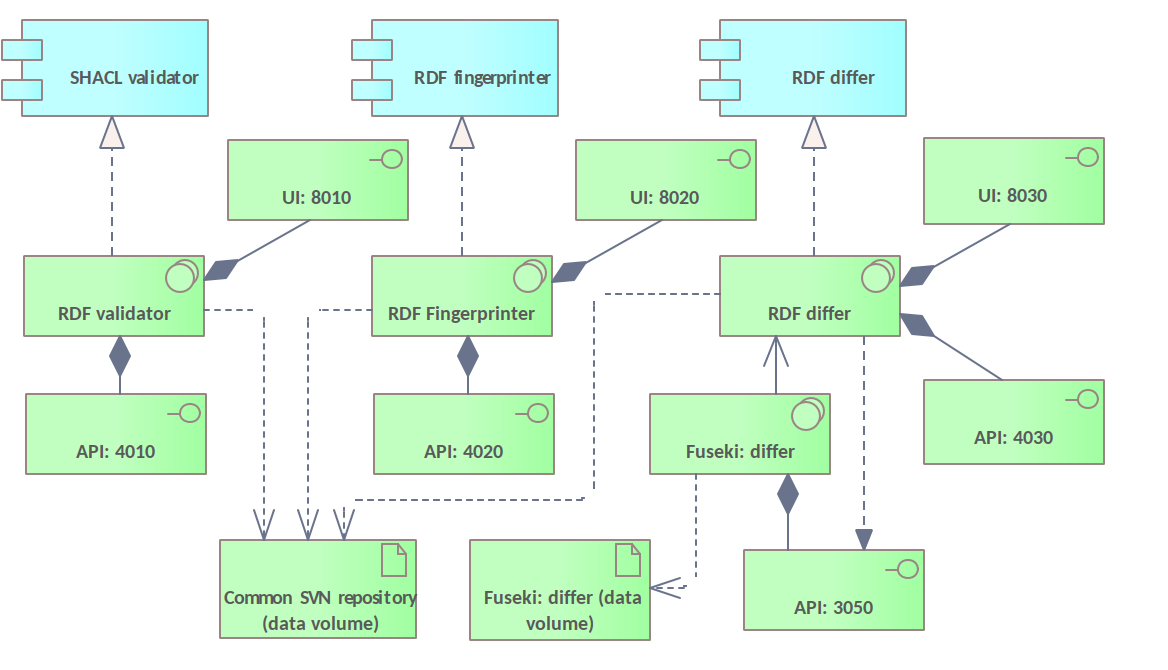
\includegraphics[width=\textwidth]{images/infra-setup/validation v2.png}
		\caption{The technology components for generation of assessment artefacts}
		\label{fig:technology-view-validation}
	\end{figure}

	The RDF validator, RDF fingerprinter and RDF differ are deployed as Docker containers and all have access to the common SVN repository volume. Doing so grants direct access to the stored files and provides the possibility to write and commit the results of their execution. For example the SHACL validator can access a file in the repository and write the validation report into the repository, next to the validated file. The RDF differ, in a similar manner, can load two versions of the same file from the common repository and compute the diff between them writing it back next to the latest version of it. The same holds for the RDF fingerprinter. 
	
	The RDF differ, does not run alone, it requires an instance of a running triple store, and in this case we choose Fuseki as it is a popular open source triple store. Another triple store can be chosen at a later stage. The reason why a triple store is necessary in the first place is that the RDF diffing operation is based on a series of SPARQL queries which can be executed only in a triple store. So in Figure \ref{fig:technology-view-validation} ``Fuseki:differ'' software is a Fuseki instance serving the RDF differ exclusively and is accessible through its API at pre-configured ports. The Fuseki instance persists its data outside the container in a dedicated volume mounted to it. 
	
	The port configuration suggested here is selected to be conflict-free and does not constitute a hard requirement and can be changed as the situation requires.
	
	A similar requirement hold for the RDF fingerprinter: a dedicated Fuseki triple store is necessary to ensure full functionality. 
	
	The RDF validator is implemented based on RDF Unit engine \citep{rdfunit-kontokostasDatabugger}. It does not have external dependencies and can validate an RDF file or a SPARQL endpoint. This makes it quite versatile because it is makes possible to execute validation operations both, on files stored in SVN common repository and on SPARQL endpoints storing intermediary data of ETL workflows and processes explained in the next section. 
	
	\section{Transformation services}
	\label{sec:technology-view-transformation}
	
	This section covers the software components necessary in the release stage when the RDF asset sources are transformed into various release artefacts. The infrastructure components and their interrelations are presented in Figure \ref{fig:technology-view-transformation}. 
	
	\begin{figure}[!h]
		\centering
		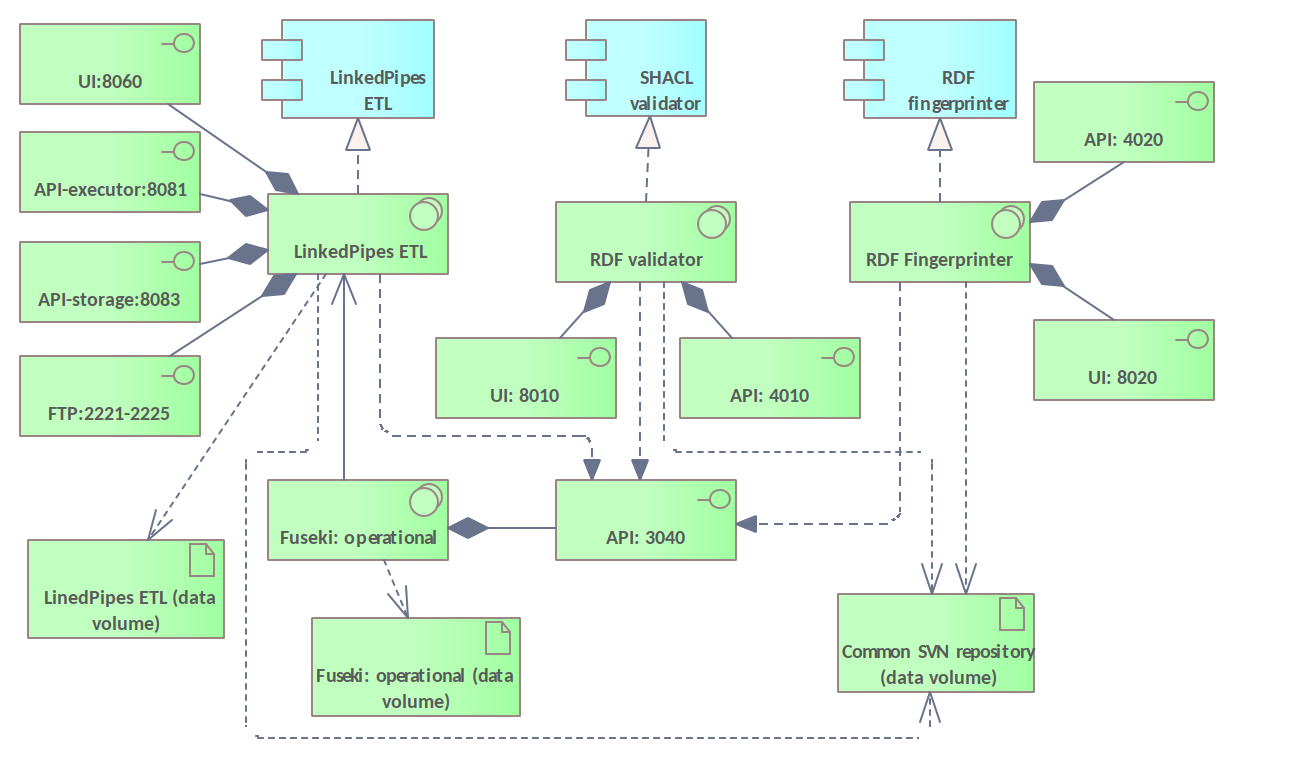
\includegraphics[width=.9\textwidth]{images/infra-setup/transformation.png}
		\caption{The technology components organisation for generation of release artefacts}
		\label{fig:technology-view-transformation}
	\end{figure}

	The key element is the LinkedPipes ETL application component (in light blue on the top of the diagram), which realises the RDF-based transformation and conversion of data. It is realised by a software element with the same name (in green below). This software exposes four technology interfaces, one of which is a user interface and the other three are technical APIs. In particular, the FTP interface is useful for debugging transformation processes while the other two for triggering and controlling the transformation process executor and the storage controller. LinkedPipes ETL can be deployed as a single container or as four separate containers, that depends on the original packaging of the software. 
	
	LinekdPipes ETL shall use the externally mounted SVN repository that serves as source for the transformation processes inputs and a place to write the final outcomes. For execution of the intermediary transformation operations and processing it needs another volume which is mounted to it. In addition it uses also a triple store for the same, operational, reasons. We propose to use a Fuseki instance dedicated to LinkedPipes ETL operations, which we call ``Fuseki: operational''. This Fuseki instance also shall use an externally mounted data volume for convenience and ease of management. 
	
	As explained in Section \ref{sec:release-new}, the transformation processes need to be controlled. Therefore the validation services described above are repeated here again to show the connection with the transformation service. The validation services have access to the ``Fuseki: operational'' instance and to the common SVN repository. Like this, a validation procedure can be triggered at any stage of the transformation process. The RDF differ is omitted from this figure because it is relevant in verifying the content implementation completeness and correctness and required human involvement. The SHACL validation and fingerprinting services can be used in a fully automated and semi-automated scenarios, and requiring little to no human intervention.
		
		
% 	\section{Reporting services}
% 	\label{sec:technology-view-reporting}
	
% 	This section covers the software components necessary for producing human readable reports on various aspects in asset publishing life-cycle. The infrastructure components and their interrelations are presented in Figure \ref{fig:technology-view-reporting}. 
	
% 	\begin{figure}[!h]
% 		\centering
% 		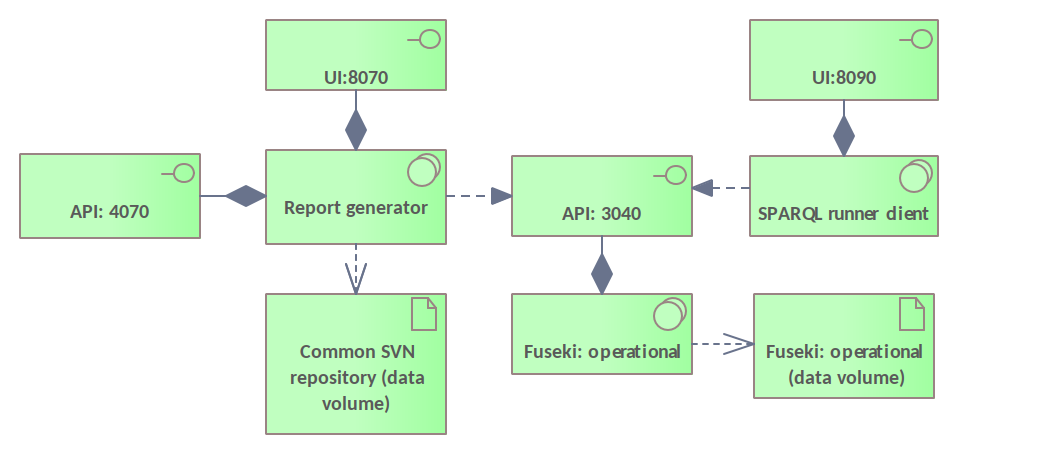
\includegraphics[width=.8\textwidth]{images/infra-setup/reporting.png}
% 		\caption{The technology components for generation of human readable artefacts}
% 		\label{fig:technology-view-reporting}
% 	\end{figure}
	
% 	The report generator is a software component which generates various reports in human readable formats such as HTML, PDF, Excel, DOCX. It does so by the virtue of predefined templates and by accessing data from the common SVN repository and from the Fuseki operational triple store. It exposes an user interface but can also access via an API.
	
% 	A very useful tool, especially fro the technical staff is a SPARQL client which can be used to execute SPARQL queries directly on SPARQL endpoints and display the results. We call it ``SPARQL runner client''. This software comes in handy when predefined queries need to be executed remotely in an automated or manual fashion outside the triple store facilities.
	
	
	\section{Service orchestration}
	\label{sec:technology-view-orchestration}
	
	This section covers the software components necessary for service orchestration across all steps of the asset publishing life-cycle. Adoption of a service orchestration application component was discussed in Section \ref{sec:implementation-application}. The infrastructure components and their interrelations are presented in Figure \ref{fig:technology-view-orchestration}. 
	
	\begin{figure}[!h]
		\centering
		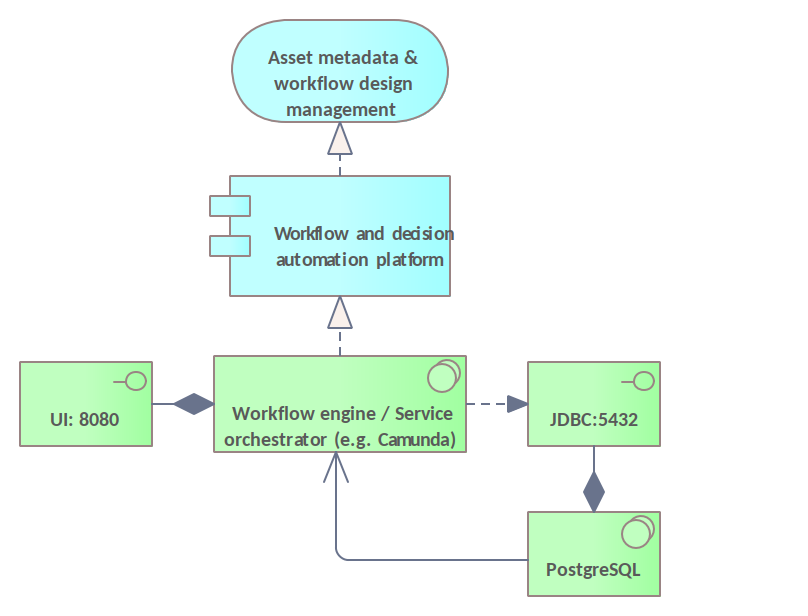
\includegraphics[width=.8\textwidth]{images/infra-setup/orchestration.png}
		\caption{The technology components for generation of human readable artefacts}
		\label{fig:technology-view-orchestration}
	\end{figure}

	In system administration, orchestration is the automated configuration, coordination, and management of computer systems and software. This can be done by designing and then executing a BPMN process. Business Process Model and Notation (BPMN) is a graphical representation for specifying business processes in a business process model. The objective of BPMN is to support business process management, for both technical users and business users, by providing a notation that is intuitive to business users, yet able to represent complex process semantics.

	We propose deployment of an instance of Camunda BPM server (or alike), which ships with tools for creating workflow and decision models, operating deployed models in production, and allowing users to execute workflow tasks assigned to them. It provides a BPMN compliant workflow engine and a Decision Model and Notation (DMN) compliant decision engine. 
	
	To support its functionality, Camunda needs a PostgreSQL database, which can be deployed in a sibling Docker container. Once Camunda BPM is deployed, BPMN workflows can be designed to access and trigger any services available on the AWS instances or any standard services offered by DIGIT. This will result in business staff being able to follow and execute entirely these workflows because the technicalities will be entirely hidden. 
		
	
\section{Conclusions}
\label{sec:conclusions}

%\bibliography{../references/references.bib}
\bibliography{docs/references/references.bib}
 
\end{document}

%This template was created by Roza Aceska.
